\documentclass[12pt,a4paper,bibliography=totocnumbered,listof=totocnumbered]{article}
% u.U. muss Koma-Skript Package ueber MikTeX deinstalliert und neu installiert werden
% Hilft das nicht, so sollte statt scrartcl die Dokumentenklasse article verwendet werden
\usepackage[backend=bibtex,style=alphabetic]{biblatex}
\usepackage[ngerman]{babel}
\usepackage[utf8]{inputenc}
\usepackage{ifthen}
\usepackage{xargs}
\usepackage{amsmath}
\usepackage{amsfonts}
\usepackage{amssymb}
\usepackage{graphicx}
\usepackage{fancyhdr}
\usepackage{tabularx}
\usepackage{geometry}
\usepackage{setspace}
\usepackage[right]{eurosym}
\usepackage[printonlyused]{acronym}
\usepackage{subfig}
\usepackage{floatflt}
\usepackage[usenames,dvipsnames]{color}
\usepackage{colortbl}
\usepackage{paralist}
\usepackage{array}
\usepackage{titlesec}
\usepackage{parskip}
\usepackage[right]{eurosym}
\usepackage[subfigure,titles]{tocloft}
\usepackage[pdfpagelabels=true]{hyperref}

\usepackage{listings}
\lstset{basicstyle=\footnotesize, captionpos=b, breaklines=true, showstringspaces=false, tabsize=2, frame=lines, numbers=left, numberstyle=\tiny, xleftmargin=2em, framexleftmargin=2em}
\makeatletter
\def\l@lstlisting#1#2{\@dottedtocline{1}{0em}{1em}{\hspace{1,5em} Lst. #1}{#2}}
\makeatother

\geometry{a4paper, top=27mm, left=20mm, right=20mm, bottom=35mm, headsep=10mm, footskip=12mm}

\definecolor{javared}{rgb}{0.6,0,0} % for strings
\definecolor{javagreen}{rgb}{0.25,0.5,0.35} % comments
\definecolor{javapurple}{rgb}{0.5,0,0.35} % keywords
\definecolor{javadocblue}{rgb}{0.25,0.35,0.75} % javadoc
\definecolor{gray}{rgb}{0.6,0.6,0.6}
 
\lstset{language=Java,
basicstyle=\ttfamily\footnotesize,
keywordstyle=\color{javapurple}\bfseries,
stringstyle=\color{javared},
commentstyle=\color{javagreen}\itshape\bfseries,
morecomment=[s][\color{javadocblue}]{/**}{*/},
numbers=left,
numberstyle=\tiny\color{gray},
stepnumber=1,
numbersep=10pt,
tabsize=3,
showspaces=false,
showstringspaces=false}
% Kopf- und Fusszeile
\renewcommand{\sectionmark}[1]{\markright{#1}}
\renewcommand{\leftmark}{\rightmark}
\pagestyle{fancy}
\lhead{}
\chead{}
\rhead{\thesection\space\contentsname}
\lfoot{}
\cfoot{}
\rfoot{\ \linebreak Seite \thepage}
\renewcommand{\headrulewidth}{0.4pt}
\renewcommand{\footrulewidth}{0.4pt}

% Vorspann
\renewcommand{\thesection}{\Roman{section}}
\renewcommand{\theHsection}{\Roman{section}}
\pagenumbering{Roman}

\newcommand{\folgen}[1]{
\ensuremath
#1
}

\newcommandx{\student}[3][]{
	\def\studentName{#1}%
	\def\studentMatnr{#2}%
	\def\studentStudiengang{#3}%
}


\newcommandx{\MyTitelseite}[8][]{
\thispagestyle{empty}

\includegraphics[scale=0.2]{pics/oth-logo.png}\hfill
\IfFileExists{#1}{\includegraphics[scale=0.5]{#1}}{}
\begin{center}
\ifthenelse{\equal{#2}{2}}{ % then
	\vspace*{2cm}
	\Large
	\textbf{Ostbayerische Technische Hochschule Regensburg}\\
	\textbf{Fakultät für Informatik und Mathematik}\\
	\vspace*{2cm}
	\Huge
	\textbf{#3}\\[1em]
	\large
	Zur Erlangung des akademischen Grades des\\
	\ifthenelse{\equal{#3}{Bachelorarbeit}}{Bachelor of Science (B.Sc.)}{Master of Science (M.Sc.)}\\
	\vspace*{1cm}
	\Large
	\textbf{#4}\\
}{ % else
	\vspace*{1cm}
	\Large
	\textbf{#4}\\
	\vspace*{2cm}
	\large
	An der Fakultät für Informatik und Mathematik der\\
	Ostbayerischen Technischen Hochschule Regensburg\\
	im Studiengang\\
	\studentStudiengang\\[2em]
	eingereichte\\
	\vspace*{1cm}
	\Large
	\textbf{#3}\\[2em]
	\large
	zur Erlangung des akademischen Grades des\\
	\ifthenelse{\equal{#3}{Bachelorarbeit}}{Bachelor of Science (B.Sc.)}{Master of Science (M.Sc.)}
	\vspace*{1cm}
	\Large
}
	\vfill
	\normalsize
	%\newcolumntype{x}[1]{>{\raggedleft\arraybackslash\hspace{0pt}}p{#1}}
	\begin{tabular}{rl}%{6cm}p{7.5cm}}
	    \rule{0mm}{1ex}\textbf{Vorgelegt von:} & \studentName \\
		\rule{0mm}{1ex}\textbf{Matrikelnummer:} & \hspace*{-0.5em}\begin{tabular}[t]{r}\studentMatnr\end{tabular} \\ 
		\ifthenelse{\equal{#2}{1}}{~\\}{\rule{0mm}{1ex}\textbf{Studiengang:} & \studentStudiengang \\[2em]}
		\rule{0mm}{1ex}\textbf{Erstgutachter:} & #5 \\ 
		\rule{0mm}{1ex}\textbf{Zweitgutachter:} & #6 \\[2em]
		\rule{0mm}{1ex}\textbf{Abgabedatum:} & #7 \\ 
	\end{tabular} 
\end{center}
\pagebreak
}

\newsavebox\mybox
\savebox\mybox{%
  \tikz{
    \draw[ultra thick,red] (-4pt,-4pt) -- (4pt,4pt);
    \draw[ultra thick,red] (-4pt,4pt) -- (4pt,-4pt);
  }%
}  

\newcommand{\TopAlign}[1]{\adjustbox{valign=t}{#1}}
\newcolumntype{T}{>{\collectcell{\TopAlign}}c<{\endcollectcell}}



\forestset{
  upsideTria/.style={
    node format={
      \noexpand\node [
      draw,
      shape=regular polygon,
      regular polygon sides=3,
      inner sep=0pt,
      outer sep=0pt,
      \forestoption{node options},
      anchor=\forestoption{anchor}
      ]
      (\forestoption{name}) {\foresteoption{content format}};
    },
    child anchor=parent,
  },
  downsideTria/.style={
     node format={
      \noexpand\node [
      draw,
      shape=regular polygon,
      regular polygon sides=3,
      shape border rotate=180,
	  inner sep=0pt,
      outer sep=0pt,
      \forestoption{node options},
      anchor=\forestoption{anchor}
      ]
      (\forestoption{name}) {\foresteoption{content format}};
    },
    child anchor=parent, 
  },
  downsideTriaTerm/.style={
     node format={
      \noexpand\node [
      draw,
      shape=regular polygon,
      regular polygon sides=3,
      shape border rotate=180,
	  inner sep=0pt,
	  outer sep=0pt,
	  fill=green,
      \forestoption{node options},
      anchor=\forestoption{anchor}
      ]
      (\forestoption{name}) {\foresteoption{content format}};
    },
    child anchor=parent, 
  },
  upsideTriaTerm/.style={
    node format={
      \noexpand\node [
      draw,
      shape=regular polygon,
      regular polygon sides=3,
      inner sep=0pt,
      outer sep=0pt,
	  fill=green,
      \forestoption{node options},
      anchor=\forestoption{anchor}
      ]
      (\forestoption{name}) {\foresteoption{content format}};
    },
    child anchor=parent,
  },
  upsideTriaYellow/.style={
    node format={
      \noexpand\node [
      draw,
      shape=regular polygon,
      regular polygon sides=3,
      inner sep=0pt,
      outer sep=0pt,
	  fill=yellow,
      \forestoption{node options},
      anchor=\forestoption{anchor}
      ]
      (\forestoption{name}) {\foresteoption{content format}};
    },
    child anchor=parent,
  },
  downsideTriaYellow/.style={
     node format={
      \noexpand\node [
      draw,
      shape=regular polygon,
      regular polygon sides=3,
      shape border rotate=180,
	  inner sep=0pt,
	  outer sep=0pt,
	  fill=yellow,
      \forestoption{node options},
      anchor=\forestoption{anchor}
      ]
      (\forestoption{name}) {\foresteoption{content format}};
    },
	child anchor=parent,
  }
}

\tikzset{
myedge/.style={
  decoration={
   markings,
   mark=at position 0.5 with \node {\usebox\mybox};
  },
  postaction=decorate
  }
}
\addbibresource{literatur.bib}


\begin{document}


% ----------------------------------------------------------------------------------------------------------
% Titelseite
% ----------------------------------------------------------------------------------------------------------
\newcommand{\studierenderName}{Korbinian Federholzner}
\student{\studierenderName}		% Studierender
{3114621}						% Matrikelnummer
{Technische Informatik}			% Studiengang

\MyTitelseite{}	% Optionales Logo des extern betreuenden Unternehmens
{1}								% Style der Titelseite (1 oder 2)
{Bachelorarbeit}				% Typ der Abschlussarbeit (\in {Bachelorarbeit, Masterarbeit})
{Entwicklung einer künstlichen Intelligenz für Brettspiele und deren Anbindung an eine Touch-Hardware über mobile Endgeräte}				% Thema der Arbeit						
{Prof.\ Dr.\ Carsten Kern}		% Betreuer
{Prof.\ Dr.\ Daniel Jobst}	% Zweitgutachter
{30.10.\the\year}				% Abgabedatum

\thispagestyle{empty}
~\pagebreak

\setcounter{page}{1} 

% ----------------------------------------------------------------------------------------------------------
% Eigensctändigkeitserklaerung
% ----------------------------------------------------------------------------------------------------------
\thispagestyle{empty}
\section*{Erklärung zur Bachelorarbeit}

\bigskip
\bigskip 
\bigskip 

\begin{enumerate}
    \item Mir ist bekannt, dass dieses Exemplar der Abschlussarbeit als Prüfungsleistung in das Eigentum der Ostbayerischen Technischen Hochschule Regensburg übergeht.
    \item Ich erkläre hiermit, dass ich diese Abschlussarbeit selbständig verfasst, noch nicht anderweitig für Prüfungszwecke vorgelegt, keine anderen als die angegebenen Quellen und Hilfsmittel benutzt sowie wörtliche und sinngemäße Zitate als solche gekennzeichnet habe.
\end{enumerate}

\bigskip 
\bigskip 
\bigskip 

Regensburg, den \today

\bigskip 
\bigskip

\line(1,0){200}
\newline
\studierenderName

% ----------------------------------------------------------------------------------------------------------
% Abstract
% ----------------------------------------------------------------------------------------------------------
\thispagestyle{empty}
\setstretch{1.15} % Zeilenspacing
\section*{Zusammenfassung}

\bigskip 


Diese Arbeit befasst sich mit der Erweiterung, der Software ReversiXT um eine Dame Künstliche Intelligenz (KI). 
Dabei wird die Anwendung um eine Verbindungsmöglichkeit für Mobile Endgeräte erweitert, welche es erlaubt, eine Verbindung
mit der Hardware herzustellen und die KI herauszufodern.
\\
Als KI Algorithmen sind MCTS und Minimax, mit Verbesserungen, wie Alpha-Beta Pruning und Zugsortierung Implementiert.
Welche im Laufe der Arbeit vorgestellt und zum Schluss, anhand einer Simulation, auf ihre Spielstärke gestest werden.
Die Implementierung der Schnittstellen, sowie Softwarekomponenten, ist Modular gehalten, was die Anwendung 
leicht um weitere Spiele, sowie KI-Algorithmen erweiterbar macht. 


% ----------------------------------------------------------------------------------------------------------
% Inhaltsverzeichnis
% ----------------------------------------------------------------------------------------------------------
\tableofcontents
\pagebreak

% ----------------------------------------------------------------------------------------------------------
% Abbildungsverzeichnis
% ----------------------------------------------------------------------------------------------------------
\lhead{}
\rhead{Abbildungsverzeichnis}
\listoffigures
\pagebreak

% ----------------------------------------------------------------------------------------------------------
% Tabellenverzeichnis (optional)
% ----------------------------------------------------------------------------------------------------------
\lhead{}
\rhead{Tabellenverzeichnis}
\listoftables
\pagebreak

% ----------------------------------------------------------------------------------------------------------
% Listingsverzeichnis (optional; Code nur, wenn wirklich sinnvoll und wichtig)
% ----------------------------------------------------------------------------------------------------------
%\lhead{}
%\rhead{Quellcodeverzeichnis}
%\lstlistoflistings
%\pagebreak

% ----------------------------------------------------------------------------------------------------------
% Abkürzungsverzeichnis (optional)
% ----------------------------------------------------------------------------------------------------------
\lhead{}
\rhead{Abkürzungsverzeichnis}
%\listoftables
\section{Abkürzungsverzeichnis}
\begin{acronym}[KDE]
\acro{KI}[KI]{künstliche Intelligenz}
\acro{GUI}[GUI]{Graphical user interface}
\acro{MCTS}[MCTS]{Monte Carlo tree search}
\acro{UML}[UML]{Unified Modeling Language}
\acro{ReversiXT}[ReversiXT]{Reversi Extreme}
\acro{UCT}[UCT]{Upper Confidence bounds applied to Trees}
\acro{TCP}[TCP]{Transmission Control Protocol}
\acro{UDP}[UDP]{User Datagram Protocol}
\acro{URL}[URL]{Uniform Resource Locator}
\end{acronym}
\pagebreak


% ----------------------------------------------------------------------------------------------------------
% Inhalt
% ----------------------------------------------------------------------------------------------------------
% Abstände Überschrift
\titlespacing{\section}{0pt}{12pt plus 4pt minus 2pt}{8pt plus 2pt minus 2pt}
\titlespacing{\subsection}{0pt}{12pt plus 4pt minus 2pt}{6pt plus 2pt minus 2pt}
\titlespacing{\subsubsection}{0pt}{12pt plus 4pt minus 2pt}{4pt plus 2pt minus 2pt}

% Kopfzeile
\renewcommand{\sectionmark}[1]{\markright{#1}}
\renewcommand{\subsectionmark}[1]{}
\renewcommand{\subsubsectionmark}[1]{}
\lhead{Kapitel \thesection}
\rhead{\rightmark}

%\onehalfspacing
\setstretch{1.15}
\renewcommand{\thesection}{\arabic{section}}
\renewcommand{\theHsection}{\arabic{section}}
\setcounter{section}{0}
\pagenumbering{arabic}
\setcounter{page}{1}

% ----------------------------------------------------------------------------------
% Kapitel: Einleitung
% ----------------------------------------------------------------------------------
\section{Einleitung}
Das Thema dieser Arbeit ist die Implementierung einer künstlichen Intelligenz für diverse
Brettspiele. Dabei soll die resultierende Software auf einem von einem Raspberry Pi gesteuerten 
Touch-Bildschirm laufen, durch welchen ein Benutzer die künstliche Intelligenz herausfordern kann.
Außerdem gibt es die Möglichkeit, sich mit der Hardware über ein mobiles Endgerät wie einem 
Smartphone zu verbinden, um die \ac{KI} oder den Spieler, der den Touch-Bildschirm bedient,
herauszufordern.

\subsection{Motivation}
Das Feld der künstlichen Intelligenz ist momentan eines der sich am schnellsten 
entwickelnden Felder der Informatik. Dabei hat die Spieltheorie schon von Anfang an eine 
große Rolle. So bieten klassische Brettspiele, wie z. B. Schach, Dame oder Mühle, nicht nur 
eine klar definierte Abstraktion von Problemen der realen Welt, sondern können auch vom 
Großteil der Bevölkerung verstanden und gespielt werden. Das Meistern eines dieser 
Brettspiele wird häufig mit einem hohem Grad an Intelligenz gleichgesetzt. Viele Algorithmen,
die in der Spieltheorie entwickelt wurden, haben sich erfolgreich auf andere Felder
der Informatik übertragen lassen. Ebenso hat sich die Art, wie Brettspiele gespielt werden, 
durch das Verwenden von künstlicher Intelligenz verändert, da die \ac{KI} Züge in Betracht 
zieht, die auf den ersten Blick recht ungewöhnlich und nachteilig aussehen, sich aber als 
extrem effektiv herausstellen. Diese Arbeit versucht eine künstliche Intelligenz für das
Brettspiel Dame zu implementieren.

\subsection{Aufgabenstellung}
\label{chap:Aufgabenstellung}
Im Rahmen der Bachelorarbeit soll eine künstliche Intelligenz entwickelt werden, welche 
das Brettspiel Dame spielen kann. Gegeben ist eine Software, bei der man in der Lage ist,
das Spiel \ac{ReversiXT} gegen eine \ac{KI} sowie sich selbst zu spielen. Diese 
Software muss um einen Game Server, die \ac{KI} und das neue Spiel in der \ac{GUI} erweitert werden.
Außerdem soll ein Benutzer in der Lage sein, sein Smartphone mit der Hardware zu 
verbinden, um eine neue sowie die alte \ac{KI} herausfordern zu können.

\subsection{Struktur dieser Arbeit}
Die Arbeit ist folgendermaßen aufgebaut: \\
Kapitel 2 befasst sich mit den Grundlagen zu Dame, sowie den verwendeten 
künstlichen Intelligenz Algorithmen. Dabei werden zu Dame auch die Grundregeln der
verwendeten Variante erläutert. Bei den \ac{KI}-Algorithmen handelt es sich um die Algorithmen, die in 
der Arbeit verwendet und miteinander verglichen werden. \\
In Kapitel 3 wird die erstellte Software Architektur vorgestellt. Dazu sind die Unterkapitel 
in die Softwarekomponenten eingeteilt und mit Hilfe von \ac{UML} Diagrammen dargestellt. 
Die verwendete Hardware, auf der die Software letztendlich zum Laufen gebracht wird, 
wird in Kapitel 4 erklärt. Das Kapitel 5 beschäftigt sich mit der Implementierung der 
Architektur und der Details, die im Architekturkapitel nicht erwähnt wurden. 
Kapitel 6 ist das Testen- und Simulationskapitel und zeigt die Methoden, welche 
zur Validierung der Software verwendet wurden.
Das siebte Kapitel Fazit und Ausblick schließt die Arbeit ab, indem es die gesamte 
Arbeit zusammenfasst und Ausblicke für die Zukunft der Software zeigt.

\pagebreak
\section{Grundlagen}
\label{chap:Grundlagen}
Dieses Kapitel gibt einen Überblick über die theoretischen Grundlagen, die für das Verständnis 
der vorliegenden Arbeit notwendig sind. Zunächst werden die Grundregeln des behandelten Brettspieles 
vorgestellt. Im Anschluss daran folgt eine Erklärung der künstlichen Intelligenz Algorithmen, welche für 
die folgenden Kapitel von großer Relevanz sind. \cite{KuenstlicheIntelligenzNorvig}

\subsection{Dame}
Dame ist eines der ältesten Brettspiele der Welt. Das Erste Spiel welches eine Ähnlichkeit zu Dame besitzt, ist das Königliche
Spiel von Ur, welches auf das Jahr 2600 v. Chr. datiert ist. Es unterscheidet sich jedoch stark von der modernen Dame.
Das Damespiel, so wie es heutzutage bekannt ist, stammt vermutlich vom Spiel Alquerque ab, welches das erste mal im 10. 
Jahrhundert erwähnt wurde. Da damals nicht jeder ein Spielbrett für Alquerque 
hatte, wurden die verfügbaren Schachbretter mit Backgammonsteinen verwendet \cite{SpieleDerWelt}.
Dieses Spiel wurde später mit Regeln wie Schlagzwang erweitert, was zur Entstehung des modernen Damespieles führte.
Auch in der heutigen Zeit gibt es noch hunderte Varianten von Dame, welche sich weltweit unterscheiden.

\subsubsection{Varianten des Spieles}
Das Spiel Dame, so wie es im deutschsprachigen Raum gespielt wird, findet auf einem 8x8 Felder Schachbrett statt. 
International wird jedoch ein 10x10 Brett und für die kanadische Version der Dame ein 12x12 Brett verwendet. 
Normalerweise können Figuren nur diagonal ziehen, es gibt jedoch
auch Abwandlungen des Spieles, wie bei der Türkischen Dame, bei welcher Spielsteine horizontal und vertikal gezogen werden können.
Das Spiel unterscheidet sich des Weiteren durch die Fähigkeiten
des Damespielsteins, welcher in einigen Varianten nur ein Feld in eine beliebige Richtung ziehen darf, in anderen 
so viele Felder wie möglich. Die Art, wie geworfen wird, ist bei diesen Abwandlungen ebenso anders. So erlauben
einige Spielarten das Schlagen eines normalen Spielsteines in die Rückwärtsrichtung, andere verbieten 
hingegen diesen Zug. Außerdem gibt es Spielformen, wie Baschni, eine Form der Russischen Dame, bei der durch Schlagen 
eines Spielsteines dieser nicht vom Spiel entfernt wird, sondern auf den Spielstein, der ihn geworfen hat, gesetzt wird. 
Wird dieser ``Turm'' aus mehreren Spielsteinen geschlagen, so wird nur der oberste Stein entfernt. 
Bei der Variante, die für diese Arbeit verwendet wird, handelt es sich um Internationale Dame, da diese 
Spielvariante im Vereinssport und internationalen Wettbewerben verwendet wird. \cite{DraughtsHistory}

\subsubsection{Internationale Dame}
Internationale Dame wird auf einem 10x10 Felder Brett mit Schachbrett-Muster gespielt,
siehe Abbildung \ref{fig:checkersboard}. Die Spielsteine
sind scheibenförmig und in zwei Farben, meist schwarz und weiß, vorhanden. Sie dürfen nur auf den dunklen
Feldern des Schachbrettes bewegt werden. Man unterscheidet zwischen zwei Arten von Spielsteinen. Normale Spielsteine, welche
nur in Richtung des Gegners bewegt werden, aber rückwärts schlagen dürfen und Damen, welche
in alle Richtungen beliebig viele Felder fahren und schlagen dürfen. Allgemein herrscht Schlagzwang
und somit muss falls ein Spieler die Möglichkeit hat zu schlagen, derjenige das auch tun.
Spielsteine, die geschlagen wurden, werden aus dem Spiel entfernt und nicht, wie bei anderen Varianten, 
auf den schlagenden Spielstein gestapelt.
Ein normaler Spielstein wird zur Dame, falls er in die hinterste Reihe des Gegners kommt.
Ziel des Spieles ist es, entweder alle Steine des Gegners zu schlagen, oder den Gegner in eine Situation
zu zwingen, in der er keine Züge mehr machen kann. \cite{InternationalCheckersRules}

\vspace{1em}
\begin{minipage}{\linewidth}
	\centering
	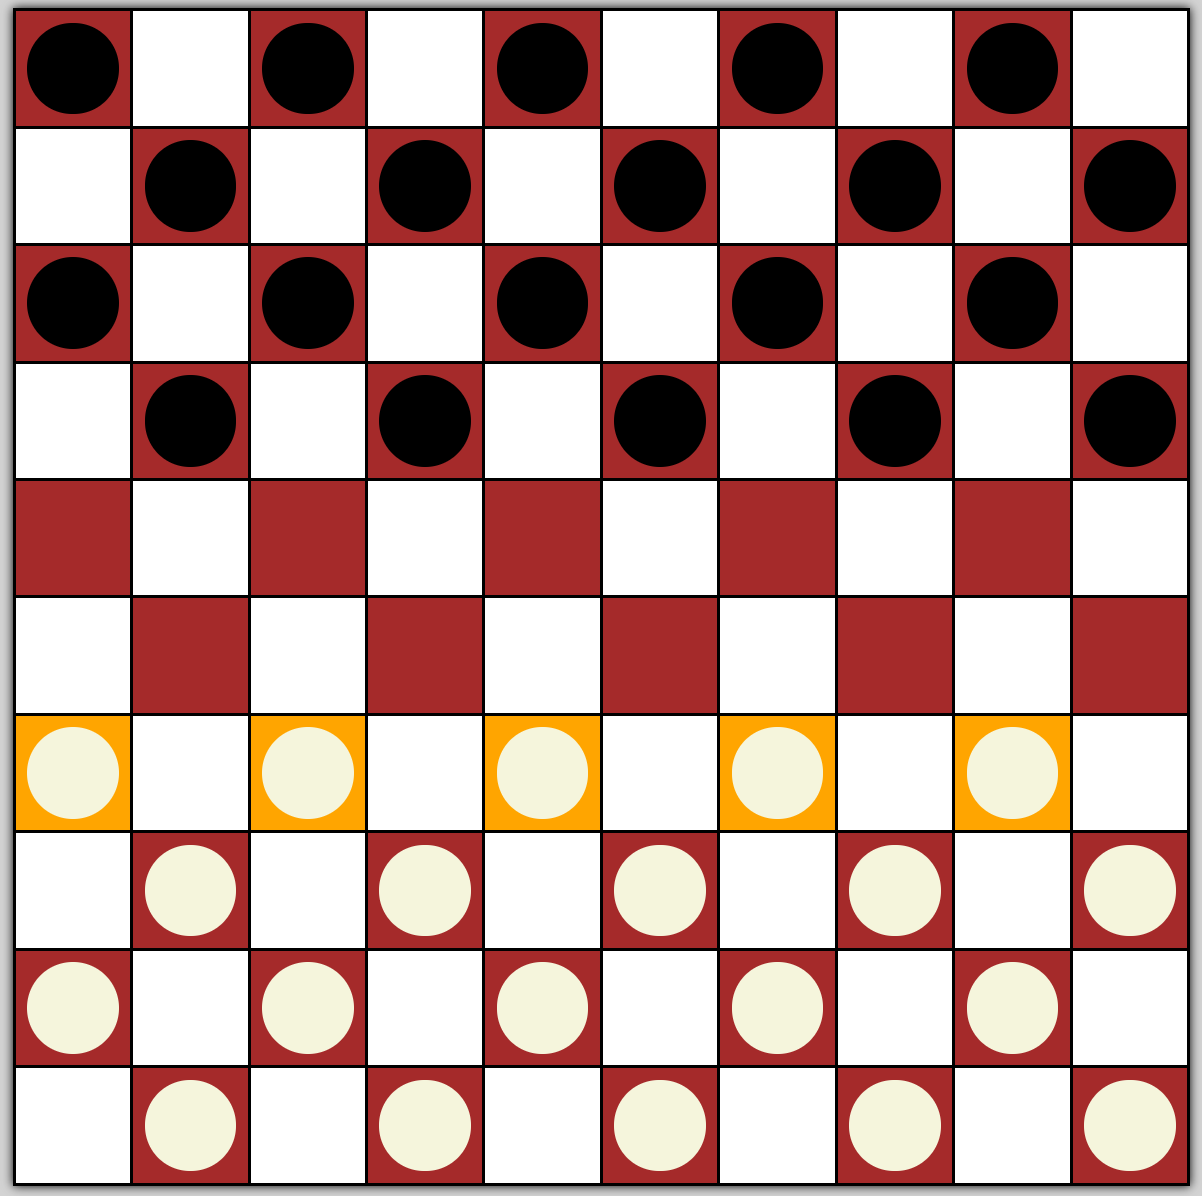
\includegraphics[width=0.5\linewidth]{pics/checkersboard.png}
	\captionof{figure}{ Das 10x10 Spielfeld aus der Anwendung }
	\label{fig:checkersboard}
\end{minipage}

\subsection{Die gegebene \ac{ReversiXT} Applikation}
\label{chap:gegebeneApp}
Wie zuvor in Kapitel \ref{chap:Aufgabenstellung} auf Seite \pageref{chap:Aufgabenstellung} erwähnt, ist das Ziel der Arbeit das Erweitern
der \ac{ReversiXT} Software um das Spiel Dame. Diese Software ist eine auf Webtechnologie basierende Anwendung, welche es dem Benutzer erlaubt,
das Spiel Reversi zu spielen. Startet man die Anwendung zum ersten Mal, wird man vom Hauptmenü, siehe Abbildung \ref{fig:ReversiMenu}, begrüßt.


\vspace{1em}
\begin{minipage}{\linewidth}
	\centering
	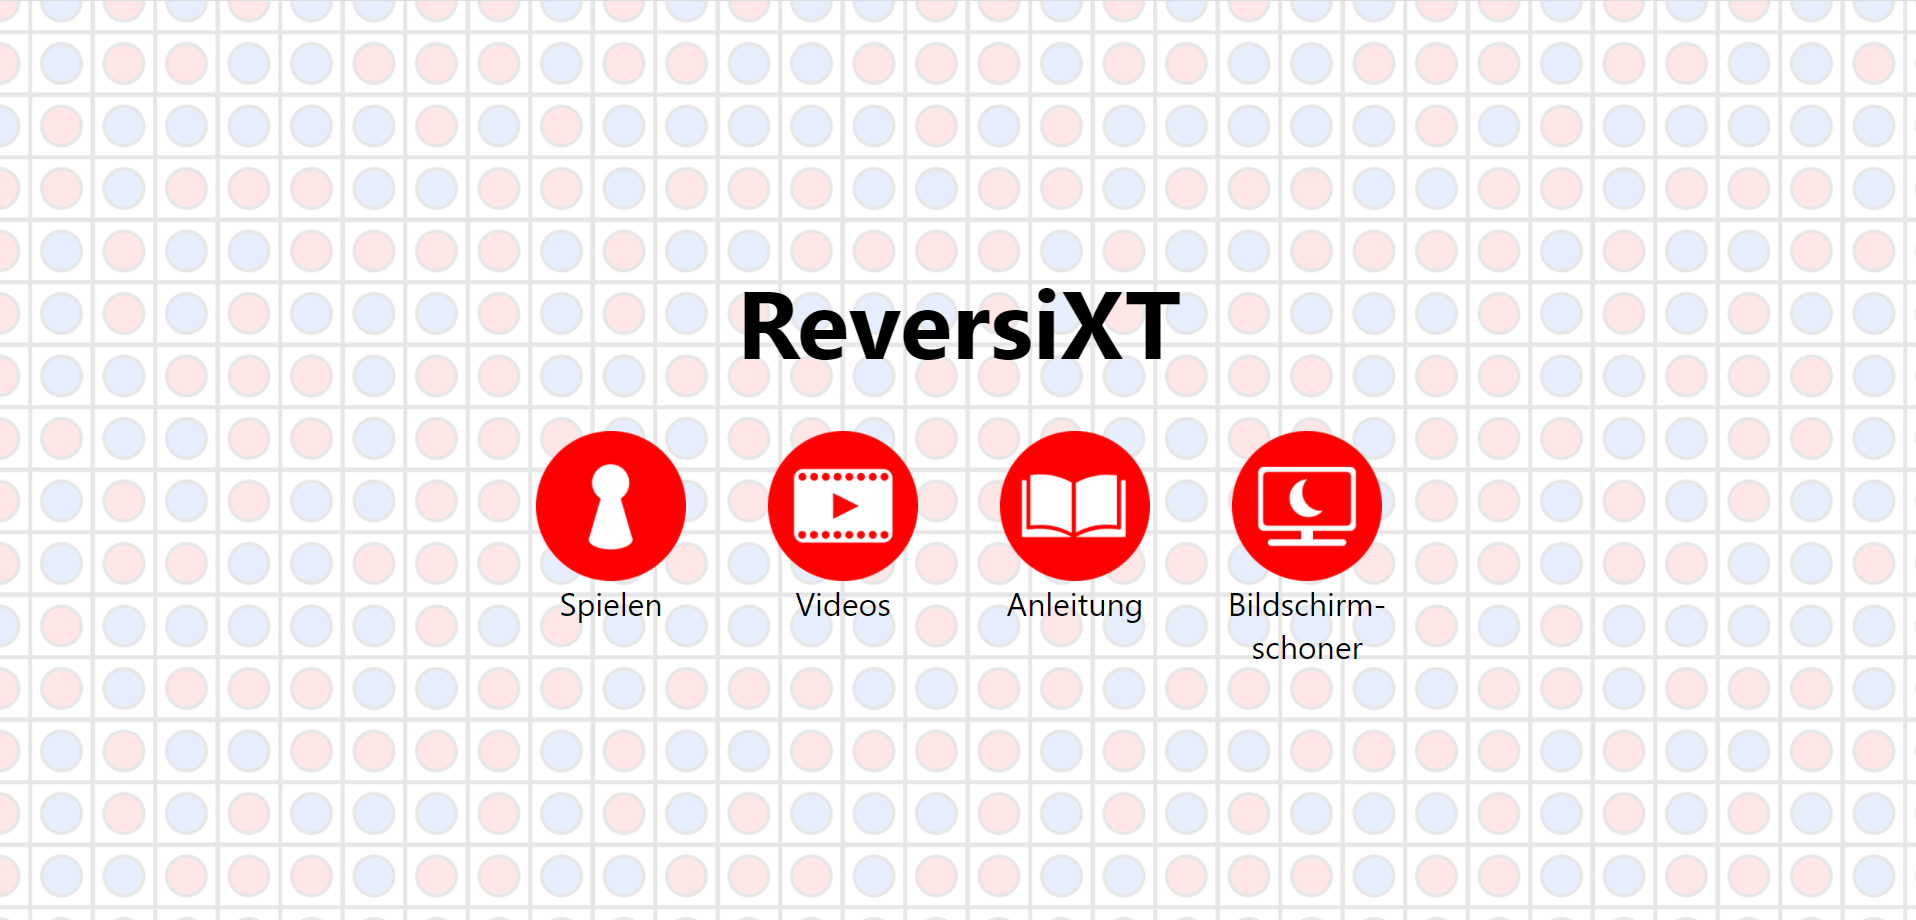
\includegraphics[width=0.7\linewidth]{pics/ReversiMenues.png}
	\captionof{figure}{ Das Hauptmenü der Anwendung}
	\label{fig:ReversiMenu}
\end{minipage}
\\

Über dieses Menü kann man entweder den Bildschirmschoner, die Anleitungen, die Videos oder ein Spiel starten. Der Bildschirmschoner 
zeigt Spiele, bei denen zwei \ac{KI}s gegeneinander spielen oder Videos, welche in der Videokategorie gespeichert sind. Wird Spielen aufgerufen, 
so wird man auf eine Seite weitergeleitet, die ein Auswahlmenü zum Starten eines Reversi Spieles bietet, siehe Abbildung \ref{fig:ReversiGameSelection}.

\vspace{1em}
\begin{minipage}{\linewidth}
	\centering
	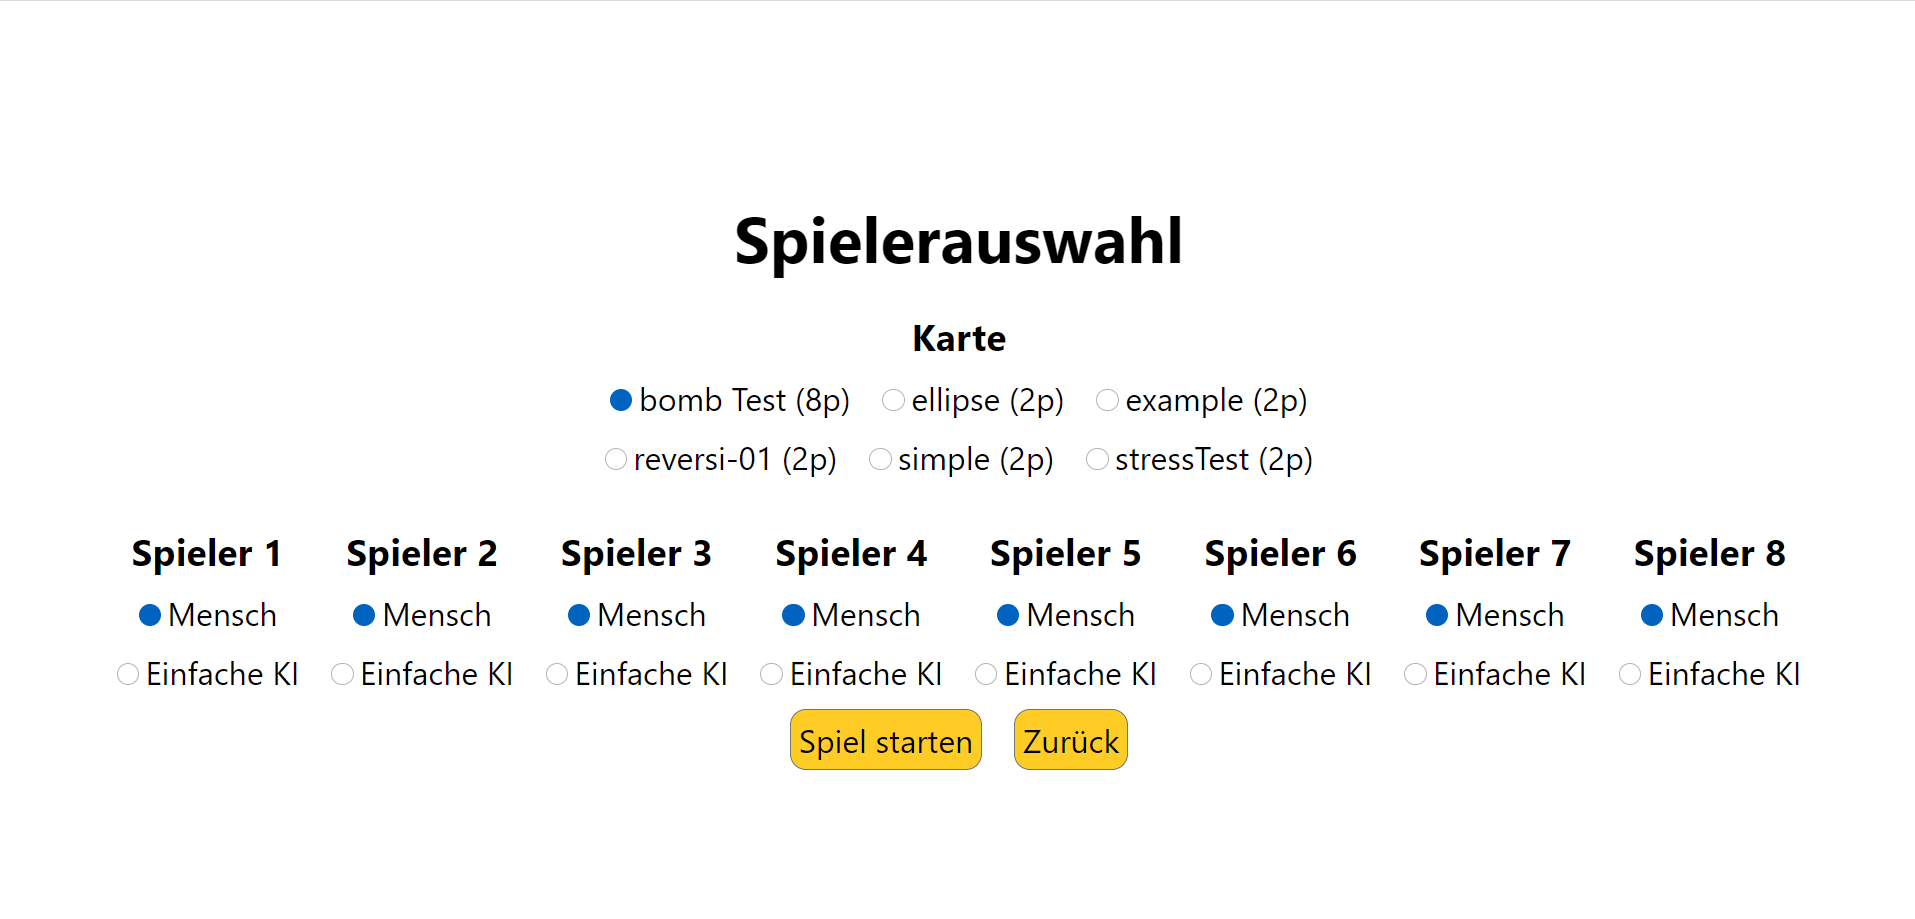
\includegraphics[width=0.7\linewidth]{pics/ReversiGameSelection.png}
	\captionof{figure}{ Das Auswahlmenü eines Reversi Spieles}
	\label{fig:ReversiGameSelection}
\end{minipage}
\\

In diesem Menü kann der Benutzer aus verschiedenen Karten und Spielern ein Spiel auswählen und starten. Jede Karte hat eine Anzahl an Spielern 
in Klammern dahinter stehen. So hat ``bomb Test (8p)'' eine Anzahl von 8 Spielern zur Auswahl. Die Auswahl der Spieler unterscheidet hierbei
zwischen ``Mensch'', dem Benutzer und ``Einfache \ac{KI}'', einer einfach implementierten Reversi \ac{KI}. Beim Drücken von ``Spiel starten'', erfolgt der Start
eines neuen Spieles und man wird auf eine Seite, die das Spielbrett darstellt, weitergeleitet, siehe Abbildung \ref{fig:ReversiGame}.

\vspace{1em}
\begin{minipage}{\linewidth}
	\centering
	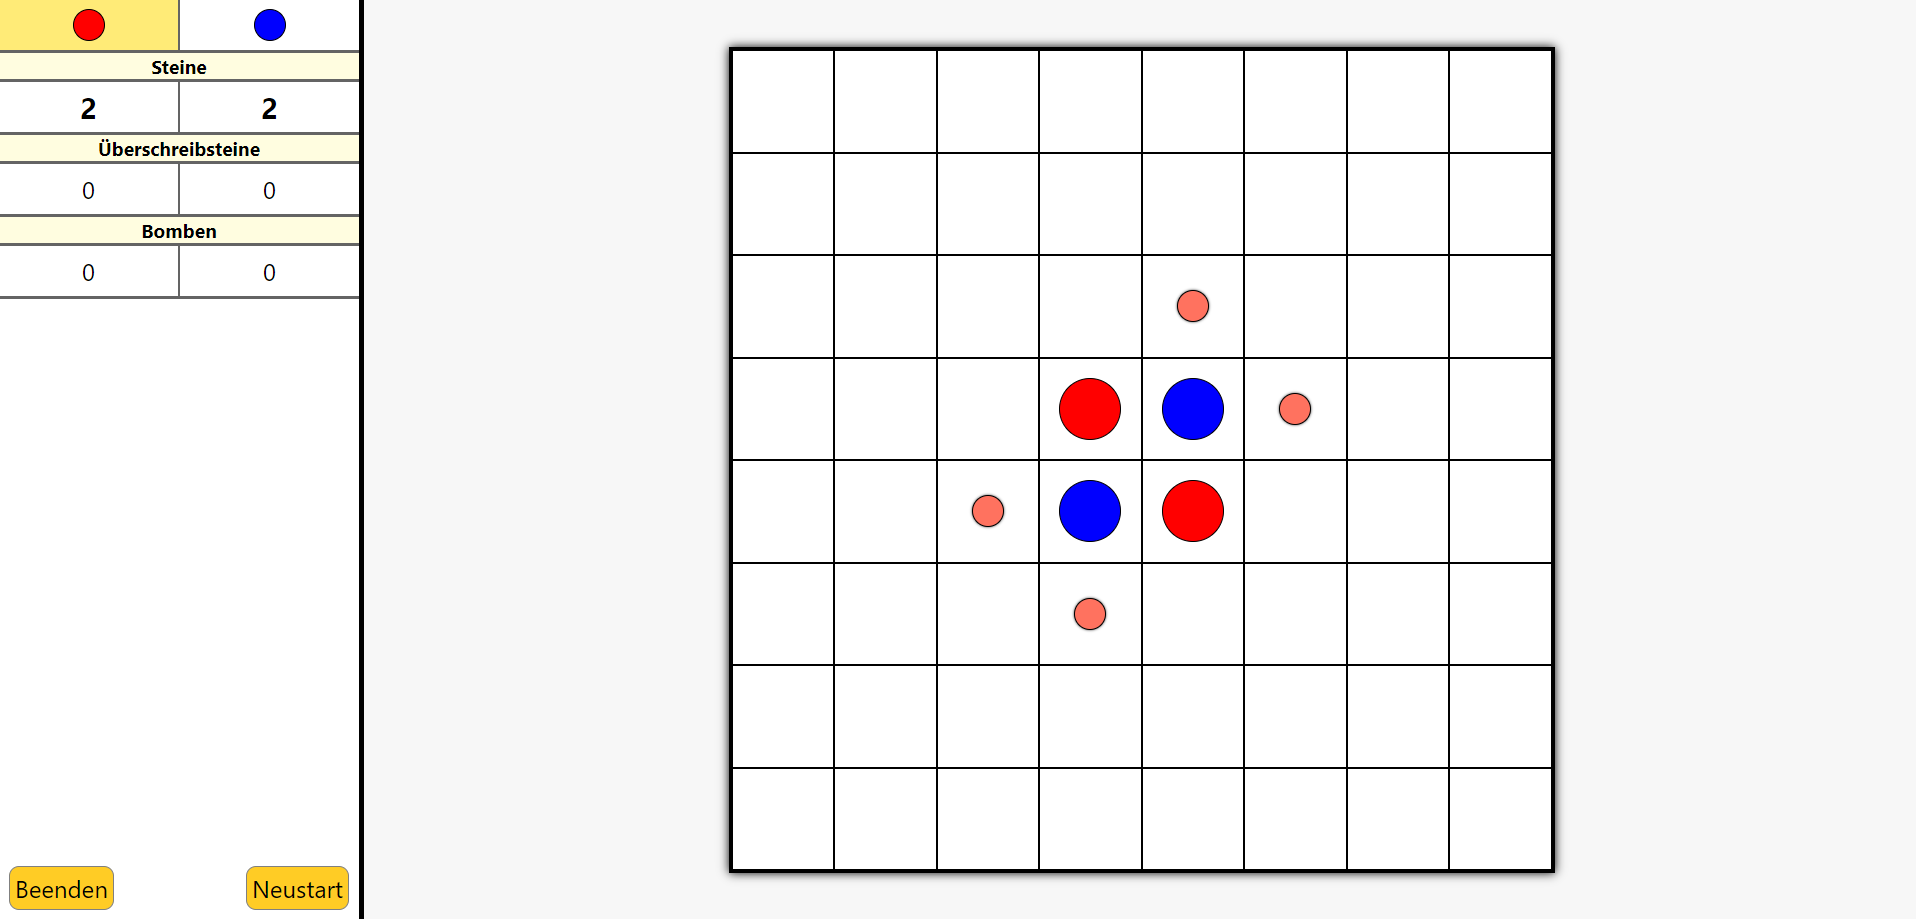
\includegraphics[width=0.7\linewidth]{pics/ReversiGame.png}
	\captionof{figure}{ Ein gestartetes Reversi Spiele }
	\label{fig:ReversiGame}
\end{minipage}
\\

Die Seite des Spieles ist unterteilt in ein Informationsmenü, welches Informationen zum laufenden Spiel und dem Spielbrett mit dem
Momentanzustand des Spieles darstellt. Falls der Benutzer an der Reihe ist, kann durch Klicken auf das Spielfeld ein neuer Zug ausgeführt werden.
Des Weiteren bietet das Informationsmenü eine Möglichkeit das Spiel neu zu starten oder zu beenden. 
Hat ein Spieler gewonnen, wird ein Info-Fenster eingeblendet, welches den Benutzer über den Sieger informiert.


\subsection{Künstliche Intelligenz Algorithmen}
Um ein Brettspiel wie Dame als künstliche Intelligenz abzubilden, gibt es viele mögliche Algorithmen.
Diese reichen von Machine Learning bis zu in dieser Arbeit verwendeten Baum-Algorithmen.
Baum-Algorithmen bei Brettspielen zeichnen sich dadurch aus, dass diese einen Spielbrettzustand als Knoten abbilden.
Dabei hat jeder Knoten einen oder mehrere Nachfolgerknoten, welche wiederum alle Züge, die aus seiner Stellung gespielt werden können, darstellen.
Die Schwierigkeit hierbei ist, die Auswahl des besten Pfades zum Sieg und dabei zu beachten, dass die Algorithmen so wenig Rechenzeit wie möglich 
dafür brauchen.

\subsubsection{Minimax}
\label{chap:Minimax}
Der Minimax Algorithmus wird verwendet, um bei zwei Spielern einen optimalen Spielzug in Spielen mit perfekter Information 
zu finden. Dazu wird eine Baumstruktur verwendet, welche den Zustand des Spielbrettes als Knoten hat, siehe Abbildung \ref{fig:minimax}.
Alle Züge, die von einer Stellung aus möglich sind, werden in den Kindknoten des jeweiligen Knotens gespeichert.
Der Wurzelknoten beschreibt den momentanen Zustand des Spieles, bei dem der Algorithmus aufgerufen wird. Die Blattknoten am Ende des Baumes
entsprechen entweder einer Stellung in der das Spiel beendet wurde, oder der Stellung bei einer Tiefe, bei der der Algorithmus 
aufgehört hat zu suchen. Die Angabe einer Tiefe ist nötig,
da Spiele wie Schach oder Dame einen extrem großen Suchbaum zur Folge hätten und das Suchen eines Endzustandes in diesem sehr viel Zeit
beanspruchen würde. \cite{MinimaxComparison}


Zum Beispiel kann der linke Baum aus Abbildung \ref{fig:minimax} durch den rechten, mit einer Suchtiefe von vier, dargestellt werden.
Dabei wird jeder Terminal-Knoten, ein Knoten bei dem das Spiel vorbei ist oder die Endtiefe erreicht wurde (im Beispiel Grün markiert), 
mit einer Bewertungsfunktion bewertet:
\begin{itemize}
    \item Normale Figur: +1 für Weiß und -1 für Schwarz
    \item Dame: +3 für Weiß und -3 für Schwarz
    \item Spielende: $\infty$ für Weiß und $-\infty$ für Schwarz
\end{itemize} 
Ein Dreieck mit der langen Seite nach unten, steht für eine Maximierung der Kindknotenwerte, das andere Dreieck für eine
Minimierung. Die Bewertungen in den Endzuständen werden nach oben durchgereicht und je nachdem, ob der Elternknoten ein Maximierer oder ein
Minimierer ist, bekommt er einen neuen Wert zugewiesen.
Im Beispiel kann man sehen, dass unabhängig davon welche Züge gewählt werden, es immer zu einem Materialverlust von Weiß kommt. Würde Weiß
die zweite Option wählen, so ist das Spiel nach dem nächsten Zug von Schwarz bereits entschieden und Weiß verliert. 

\begin{figure}[H]
\centering
\scalebox{0.38}
{%
\begin{adjustbox}{valign=t}
\begin{forest}
[{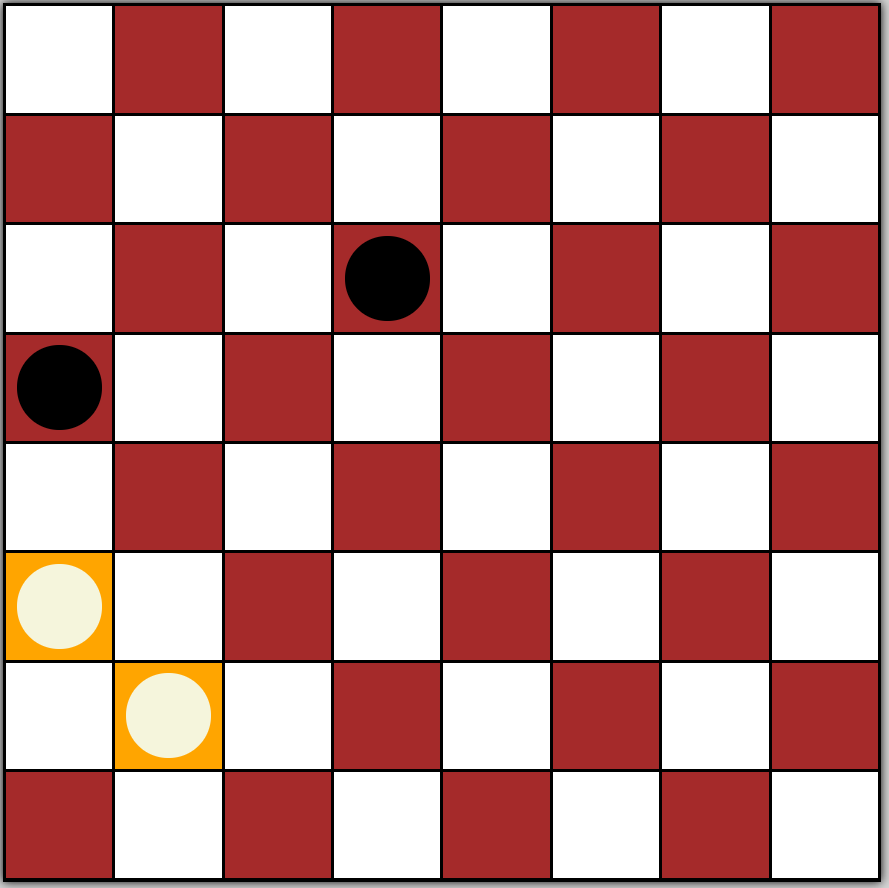
\includegraphics[scale=0.2]{pics/root.png}}
    [{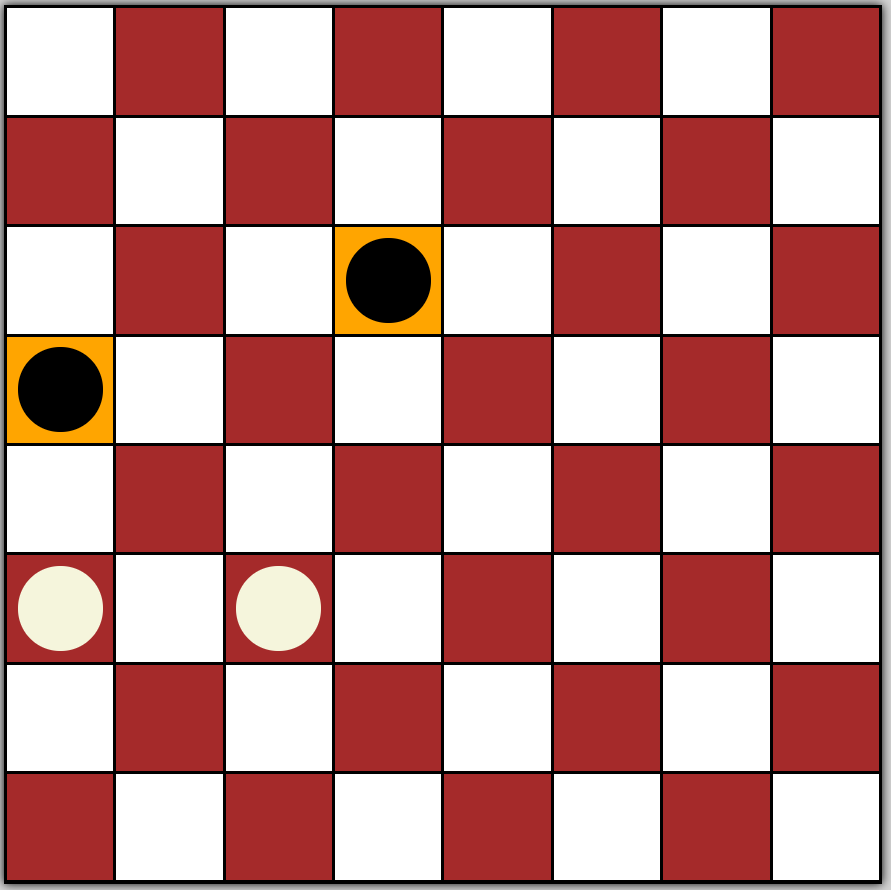
\includegraphics[scale=0.15]{pics/1goodmove.png}}
        [{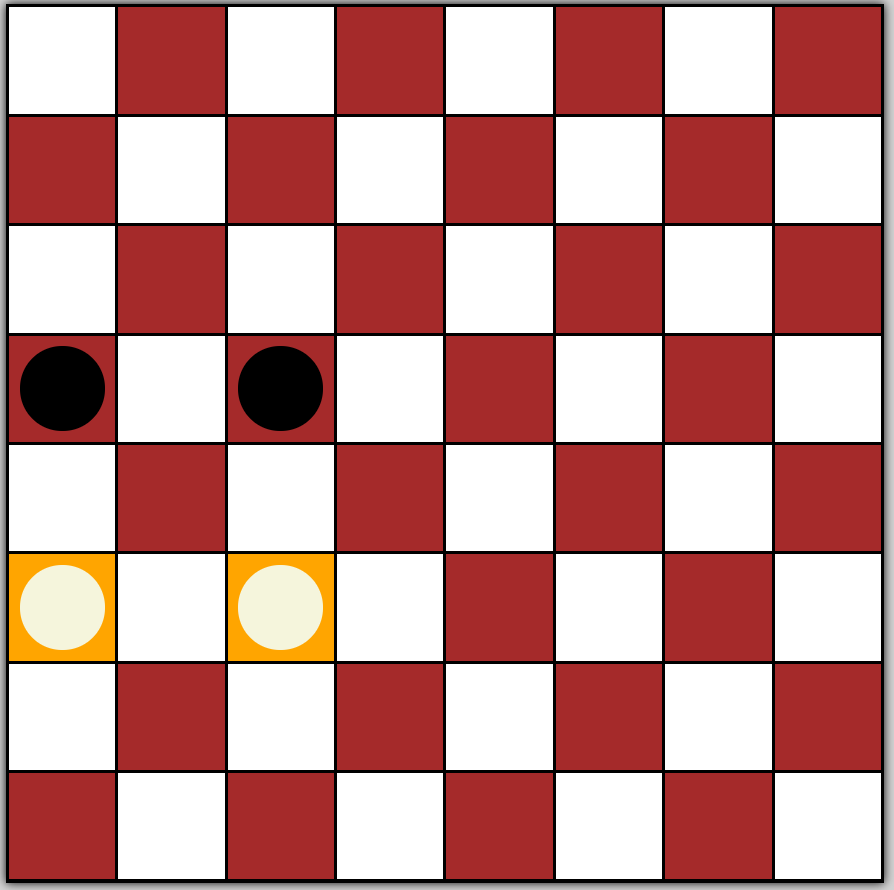
\includegraphics[scale=0.15]{pics/21goodmove.png}}
            [{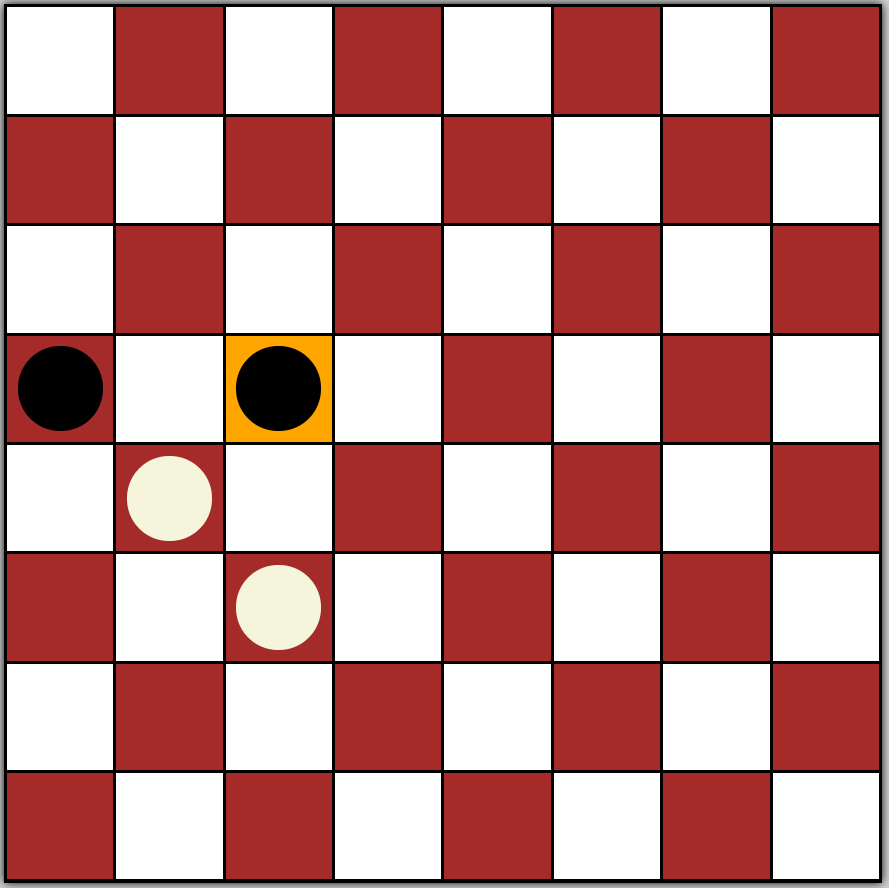
\includegraphics[scale=0.12]{pics/311goodmove.png}}
                [\vdots]
            ]
            [{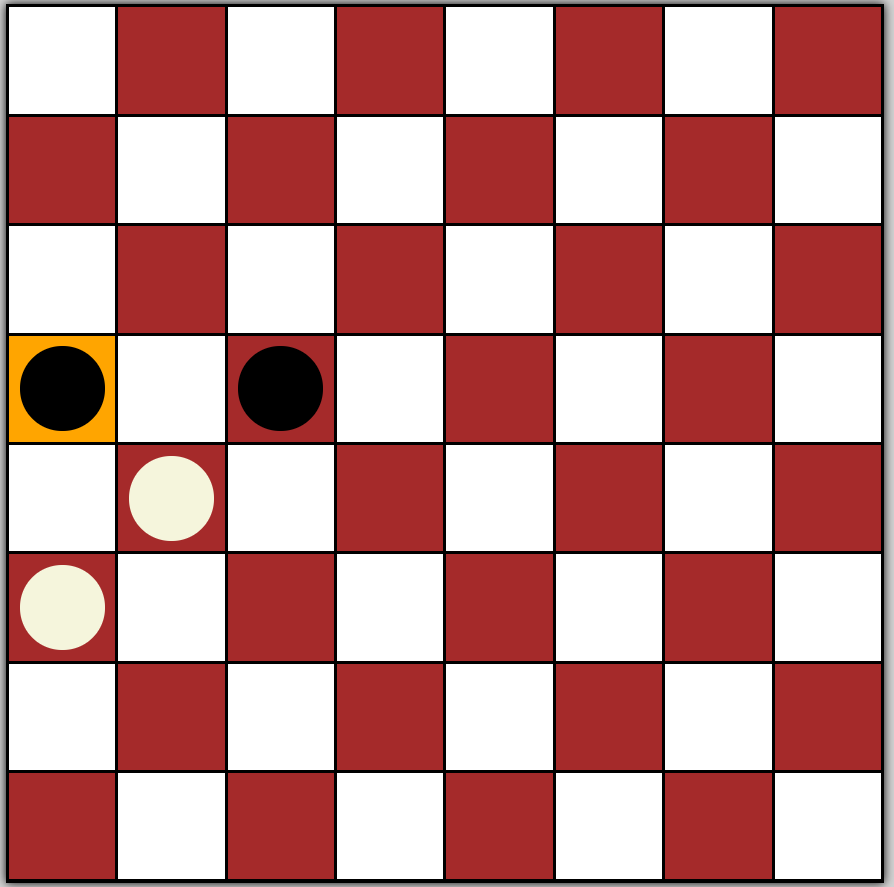
\includegraphics[scale=0.12]{pics/312goodmove.png}}
                [\vdots]
            ]
            [{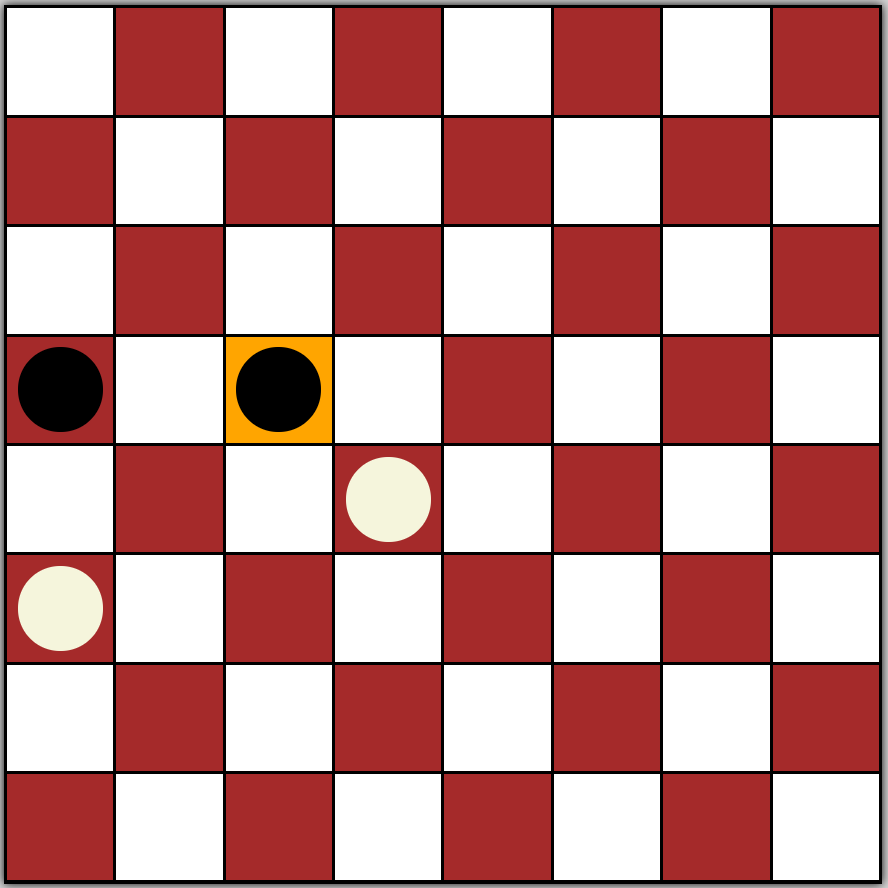
\includegraphics[scale=0.12]{pics/313goodmove.png}}
                [\vdots]
            ]
        ]
        [{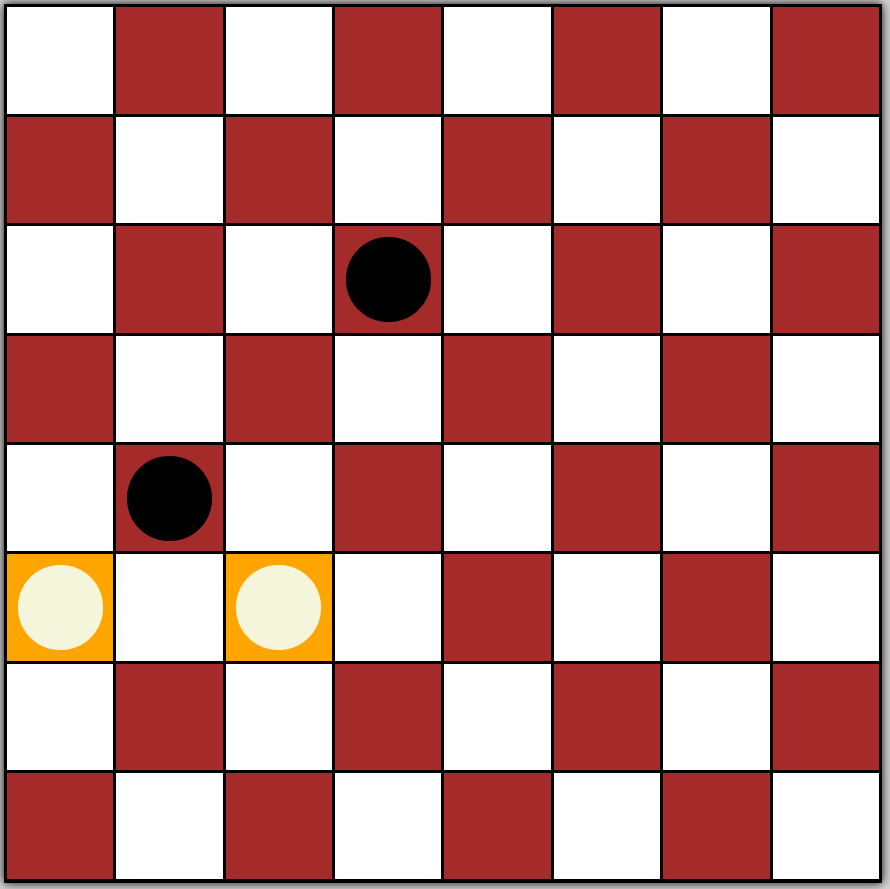
\includegraphics[scale=0.15]{pics/22badmove.png}}
            [{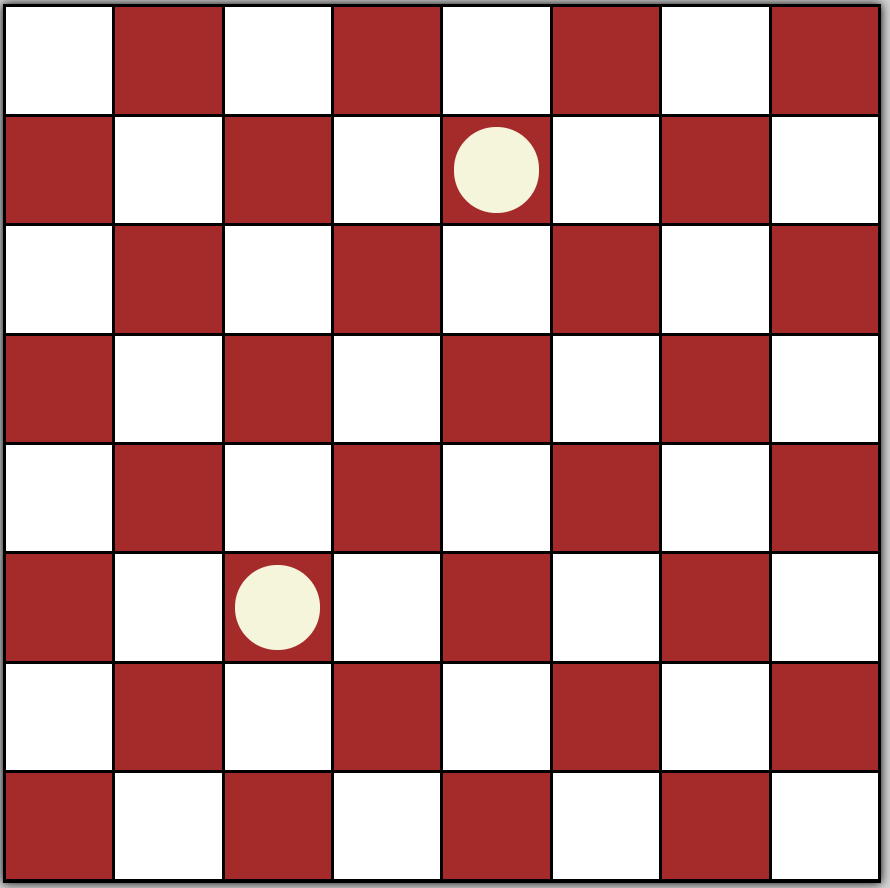
\includegraphics[scale=0.12]{pics/322badmove.png}}]
            [{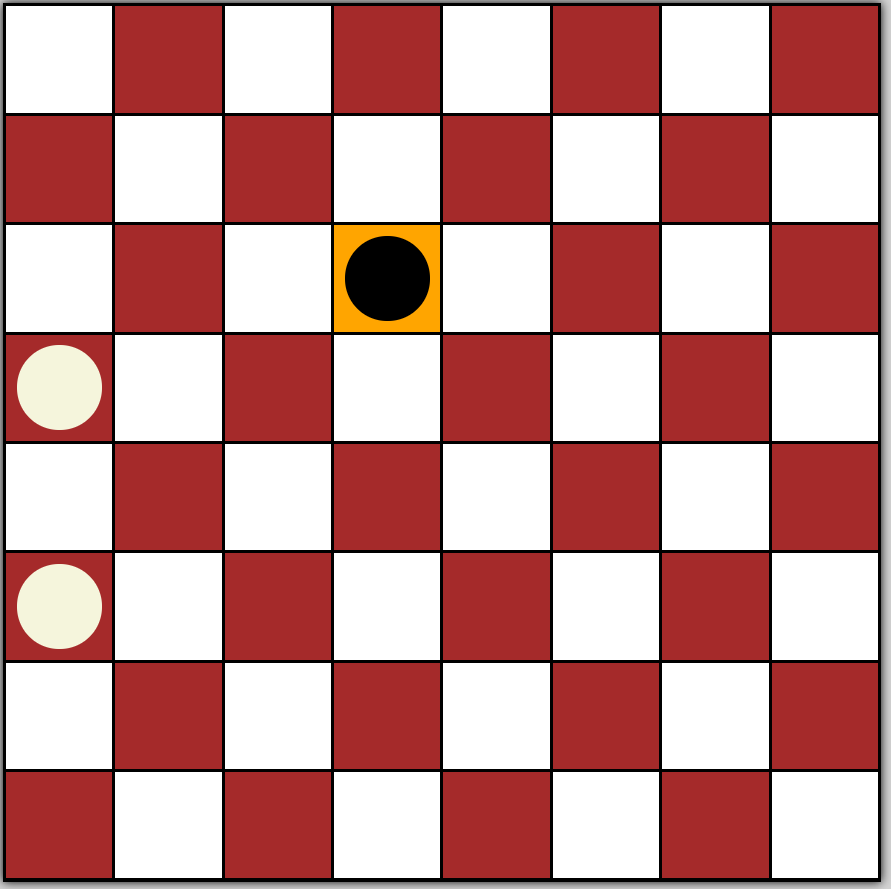
\includegraphics[scale=0.12]{pics/321badmove.png}}
                [\vdots]
            ]
        ]
    ]
    [{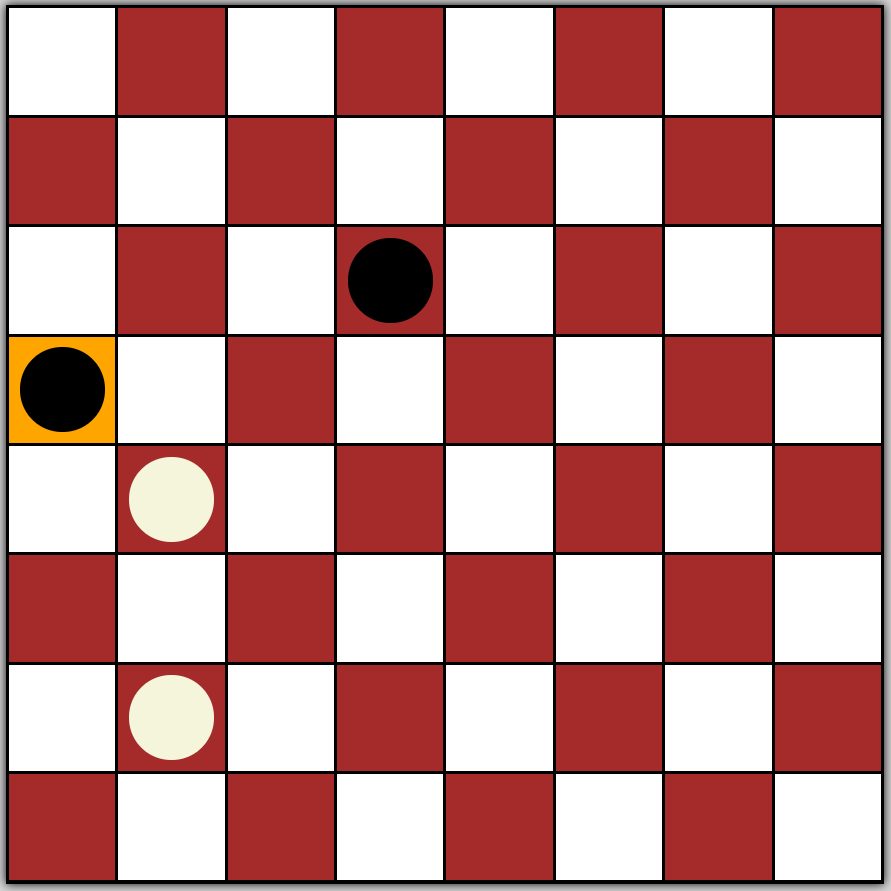
\includegraphics[scale=0.15]{pics/1badmove.png}}
        [{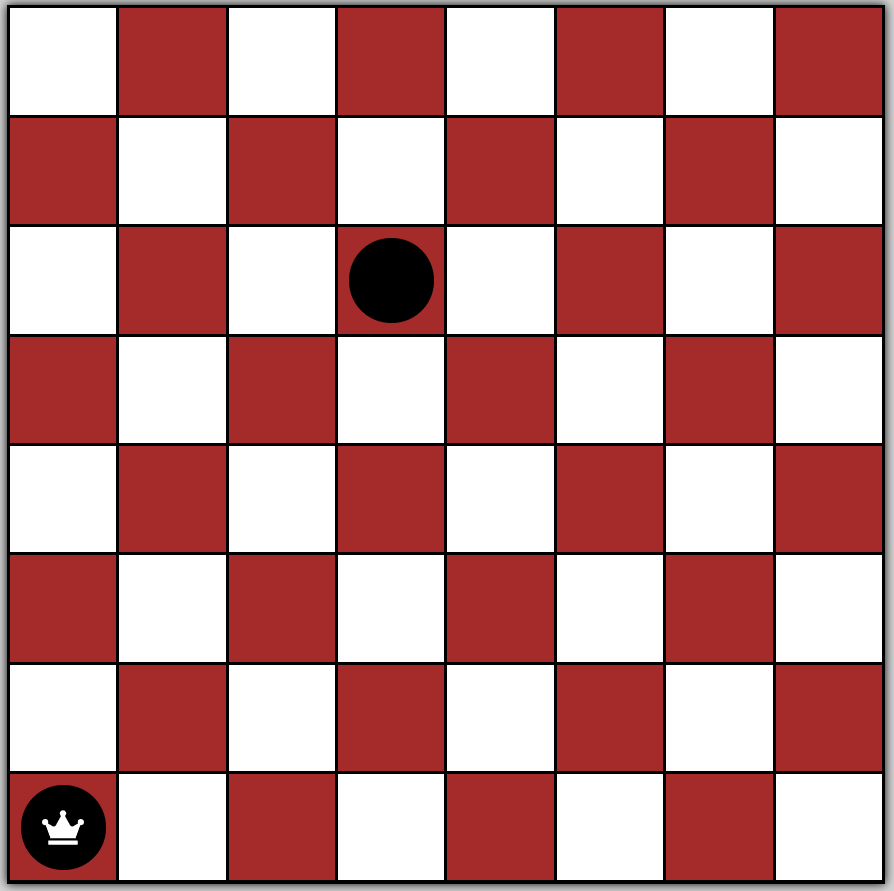
\includegraphics[scale=0.15]{pics/2winAfter1badmove.png}}]
    ]
]
\end{forest}
\end{adjustbox}\qquad
}
\centering
\scalebox{1.25}
{%
\begin{adjustbox}{valign=t}
\begin{forest}
    [-1, upsideTria
        [-1, downsideTria
            [-1, upsideTria
                [-1, downsideTria
                    [-1, upsideTriaTerm]
                ]
                [-1, downsideTria
                    [-1, upsideTriaTerm]
                ]
                [-1, downsideTria
                    [-1, upsideTriaTerm]
                ]
            ]
            [$\infty$, upsideTria
                [$\infty$, downsideTriaTerm]
                [-1, downsideTria
                    [-1, upsideTriaTerm]
                    [-1, upsideTriaTerm]
                ]
            ]
        ] 
        [{\fontsize{9}{8}\selectfont $-\infty$}, downsideTria
            [{\fontsize{9}{8}\selectfont $-\infty$}, upsideTriaTerm]
        ] 
    ]
\end{forest}
\end{adjustbox}
}
\caption{Minimax Baum, links Darstellung der in den Konten gespeicherten Spielfelder, rechts bewertete Knoten}
\label{fig:minimax}
\end{figure}

\subsubsection{Iterative Deepening}
\label{chap:IterativeDeepening}
In komplexeren Spielen, wie Go, Schach oder Dame, ist es wegen des Rechenaufwands sehr schwer, den kompletten Baum von Minimax bis zu den
Endzuständen aufzubauen. Deswegen wird in diesen Spielen der Baum nur bis zu einer gewissen Tiefe aufgebaut. Da es aber bei gleicher
Tiefe für verschiedene Stellungen zu unterschiedlichen Dauern der Suche kommen kann, ist es problematisch eine fixe Suchtiefe anzugeben, 
vor allem wenn mit Zeitlimits gearbeitet wird. Das Iterative Deepening hilft hierbei. Der Ablauf des Algorithmus ist wie folgt:
Zuerst führe Minimax für eine Tiefe von 1 aus. Danach, verwerfe alle generierten Knoten des Baumes und starte erneut vom Anfang, aber dieses
Mal bis zu einer Tiefe von 2. Dieses Verwerfen und Neustarten wird so oft wiederholt, bis ein Zeitlimit erreicht wird, siehe Abbildung \ref{fig:IterativeDeepening}. 
Bevor neugestartet wird der letzte aufgebaute Baum zwischengespeichert und falls Minimax bis zum Ablauf des Zeitlimits nicht fertig ist,
die momentane Berechnung verworfen und der letzte gespeicherte Baum verwendet. Ein Nachteil dieser Methode ist, dass 
der Rechenaufwand der ersten Tiefen verschwendet wird, da diese Ergebnisse verworfen werden. Jedoch beeinflusst diese 
verschwendete Rechenzeit nicht die asymptotische Laufzeit des Algorithmus, da die meiste Arbeit in der untersten Tiefe der 
Suche gebraucht wird. \cite{IterativeDeepening}.

\begin{figure}[H]
\centering
\begin{tabular}{*{6}{|T}}
    Tiefe 1 & Tiefe 2 & Tiefe 3 \\
    \begin{forest}
        [$\triangle$
            [$\nabla$] 
            [$\nabla$] 
        ]
    \end{forest}
    &
    \begin{forest}
        [$\triangle$
            [$\nabla$ 
                [$\triangle$]
                [$\triangle$]
            ]
            [$\nabla$ 
                [$\triangle$]
            ]
        ]
    \end{forest}
    &
    \begin{forest}
        [$\triangle$
            [$\nabla$ 
                [$\triangle$
                    [$\nabla$]
                ]
                [$\triangle$
                    [$\nabla$]
                    [$\nabla$]
                ]
            ]
            [$\nabla$ 
                [$\triangle$
                    [$\nabla$]
                    [$\nabla$]
                    [$\nabla$]
                ]
            ]
        ]
    \end{forest}
    \\
\end{tabular}
\caption{Ablauf des Iterative Deepening}
\label{fig:IterativeDeepening}
\end{figure}

\subsubsection{Alpha-Beta-Pruning}
\label{chap:alphaBeta}
Das Alpha-Beta-Pruning ist eine Optimierung zum Minimax Algorithmus. Die Idee des Algorithmus ist, 
dass manche Zweige des Suchbaums nicht untersucht werden müssen, da für den anderen Spieler diese
Züge nicht in Frage kommen. Hierbei ist $\alpha$ der Wert für den Spieler, für den die niedrigen Werte 
besser sind und $\beta$ für den anderen Spieler. Für jeden Knoten, je nachdem, ob er ein maximierender
oder ein minimierender Knoten ist, wird überprüft, ob ein Kindknoten, welcher einen neuen Wert
erhalten hat, nicht mehr vom Knoten beachtet werden muss. Der Vorteil des Alpha-Beta-Prunings zu Minimax ist, 
dass der verbrauchte Speicher weniger wird, da vom Baum Zweige nicht beachtet werden müssen.
Dies hat wiederum zur Folge, dass die Ausführungszeit des Algorithmus schneller ist und gleichzeitig auch dasselbe 
Ergebnis wie Minimax zur Folge hat.
\cite{AlphaBeta}

Wenn man Abbildung \ref{fig:minimax} als Beispiel nimmt und den Alpha-Beta-Pruning Algorithmus anwendet,
so kann der Zweig mit dem Wert $\infty$ ignoriert werden, siehe Abbildung \ref{fig:AlphaBeta}. Der gelbe Knoten bekommt,
durch seinen linken Zweig vorübergehend eine -1 zugewiesen. Da der Knoten des rechten Zweiges ein Maximierer ist, also immer den Wert des
Kindknotens mit dem höchsten Wert nimmt und dieser bereits einen Knoten mit dem Wert $\infty$ gefunden hat, wird sein Wert 
definitiv mindestens $\infty$ sein. Der restliche rechte Zweig des gelben Knotens kann nun ignoriert werden, da der linke Zweig mit
-1 definitiv kleiner sein wird.

\begin{figure}[H]
\centering
{%
\begin{forest}
    [-1 , upsideTria
        [-1, downsideTriaYellow
            [-1, upsideTria
                [-1, downsideTria
                    [-1, upsideTriaTerm]
                ]
                [-1, downsideTria
                    [-1, upsideTriaTerm]
                ]
                [-1, downsideTria
                    [-1, upsideTriaTerm]
                ]
            ]
            [$\infty$, upsideTria, edge={myedge}
                [$\infty$, downsideTriaTerm]
                [?, downsideTria]
            ]
        ] 
        [{\fontsize{9}{8}\selectfont $-\infty$}, downsideTria
            [{\fontsize{9}{8}\selectfont $-\infty$}, upsideTriaTerm]
        ] 
    ]
\end{forest}
}
\caption{Gewinn durch Alpha-Beta-Pruning}
\label{fig:AlphaBeta}
\end{figure}

\subsubsection{Zugsortierung}
\label{chap:Zugsortierung}
Die Zugsortierung ist eine Erweiterung zur Alpha-Beta Suche.
Da Alpha-Beta-Pruning abhängig von der Reihenfolge ist, in der die Zustände untersucht werden, ist es sinnvoll,
die Nachfolger zu wählen, welche die besten Werte erbringen. Den besten Nachfolger findet man, indem man eine
weitere Bewertungsfunktion einbaut, die nicht so genau wie die Bewertungsfunktion an den Terminalknoten sein muss. 
Wenn ein Knoten also alle möglichen Nachfolgezüge als Kinder bekommt, werden auf diese die vereinfachte Bewertungsfunktion
angewandt und je nach Ergebnis der Funktion die Nachfolger sortiert. Da der beste Zug nun
sehr weit am Anfang steht, ist es sehr wahrscheinlich, dass die anderen Züge durch Alpha-Beta-Pruning ignoriert werden.
\cite{KuenstlicheIntelligenzNorvig}

Auf der linken Seite der Abbildung \ref{fig:Sorting} kann man erkennen, dass Alpha-Beta-Pruning keinen Effekt 
auf die beiden gelben Knoten hätte. Ändert man jedoch die Reihenfolge der Knoten, kann der Knoten mit dem Wert 42
ignoriert werden. Bei der Bewertungsfunktion könnte man die bedrohten Figuren als Faktor haben, um auf dieses Ergebnis zu kommen.


\begin{figure}[H]
\centering
{%
\begin{forest}
    [-1, upsideTria
        [-1, downsideTria
            [$\infty$, upsideTriaYellow
                [$\infty$, downsideTriaTerm]
                [-1, downsideTria
                    [-1, upsideTriaTerm]
                    [-1, upsideTriaTerm]
                ]
            ]
            [-1, upsideTriaYellow
                [-1, downsideTria
                    [-1, upsideTriaTerm]
                ]
                [-1, downsideTria
                    [-1, upsideTriaTerm]
                ]
                [-1, downsideTria
                    [-1, upsideTriaTerm]
                ]
            ]
        ] 
        [{\fontsize{9}{8}\selectfont -$\infty$}, downsideTria
            [{\fontsize{9}{8}\selectfont -$\infty$}, upsideTriaTerm]
        ] 
    ]
\end{forest}
\raisebox{1\height}{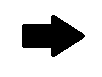
\includegraphics{pics/ArrowRight.png}}
\begin{forest}
    [-1 , upsideTria
        [-1, downsideTria
            [-1, upsideTriaYellow
                [-1, downsideTria
                    [-1, upsideTriaTerm]
                ]
                [-1, downsideTria
                    [-1, upsideTriaTerm]
                ]
                [-1, downsideTria
                    [-1, upsideTriaTerm]
                ]
            ]
            [$\infty$, upsideTriaYellow, edge={myedge}
                [$\infty$, downsideTriaTerm]
                [?, downsideTria]
            ]
        ] 
        [{\fontsize{9}{8}\selectfont -$\infty$}, downsideTria
            [{\fontsize{9}{8}\selectfont -$\infty$}, upsideTriaTerm]
        ] 
    ]
\end{forest}
}
\caption{Beispiel einer Zugsortierung}
\label{fig:Sorting}
\end{figure}

\subsubsection{Monte Carlo Tree Search (MCTS)}
\label{chap:MCTS}
Der Monte Carlo Tree Search Algorithmus ist ein heuristischer Algorithmus, bei welchem von einem
Zustand eines Spieles zufällig endlich viele Simulationen durchgeführt werden. Die Simulation endet, wenn
ein Ergebnis des simulierten Spieles feststeht. Das Wiederholen der Simulationen aus verschiedenen Knoten
hat zur Folge, dass das Ergebnis immer genauer wird. Am Ende wird der Knoten gewählt, bei dem die 
Simulationen die besten Ergebnisse für den momentanen Spieler gezeigt haben. Ein Vorteil des 
\ac{MCTS}-Algorithmus gegenüber Minimax ist, dass erst am Ende eines Durchlaufs eine Bewertungsfunktion
benötigt wird. Allgemein besteht der Algorithmus aus vier Schritten:
\begin{itemize}
    \item \textit{Selektion}: Versucht wird, einen Zustand zu finden, der noch erweiterbar ist, also
        kein Endzustand ist und noch nicht besuchte Züge hat.
    \item \textit{Expansion}: Der Spielbaum wird zufällig um einen noch nicht besuchten Zug erweitert.
    \item \textit{Simulation}: Von dem gewählten Knoten aus wird nun ein Spiel zufällig bis zum Ende 
        simuliert. 
    \item \textit{Backpropagation}: Das Ergebnis der Simulation wird den vorhergehenden Knoten mitgeteilt
        und diese werden mit diesem aktualisiert.
\end{itemize}
Da man im Normalfall nicht beliebig viel Zeit hat, alle Möglichkeiten zu simulieren, versucht man die limitierte Zeit
so effektiv wie möglich zu nutzen, um die richtigen Knoten zum Expandieren zu wählen. Dazu wird der \ac{UCT} verwendet.
Die \ac{UCT} Formel lautet:
\begin{align}
	w + c \sqrt{\frac{\log{N}}{n}}
\end{align}
Wobei $w$ die prozentuale Anzahl an Gewinnen des Knotens, $N$ die Anzahl der gesamten Expansionen und $n$ nur die Expansionen an dem 
betrachteten Knoten sind. Die Aufgabe der \ac{UCT} Formel ist das Erreichen von im Konflikt stehenden Zielen. Das erste Ziel ist es, die Knoten, die bisher die 
höchsten Chancen auf den Gewinn haben, tiefer zu simulieren, um eine bessere Genauigkeit des besten Zuges zu haben.
Das zweite Ziel ist, Knoten, die noch nicht sehr oft besucht worden sind, genauer zu untersuchen, da diese vielversprechender sein könnten als gedacht.
Für die Balancierung der beiden Ziele gibt es den Parameter $c$ \cite{DeepLearingGo}.

Als Beispiel wird die zuvor verwendete Stellung aus \ref{fig:minimax} benutzt, aus welcher der \ac{MCTS}-Baum in Abbildung \ref{fig:MCTSTree} entsteht.
``B'' steht für die Siege aus schwarzer und ``W'' für Siege aus weißen Sicht, nach der Beendigung von 33 Simulationen.  
Weiß entscheidet sich in diesem Baum für den gelben Knoten, da dieser bei Betrachtung der Gewichtung von Siegen eine höhere
Gewinnchance für ihn aufweist.

\begin{figure}[H]
\centering
{%
\begin{forest}
    for tree={%
        edge={->},
    }
    [B:27 W:6, circle, draw
        [B:19 W:6, circle, fill=yellow, draw
            [B:12 W:1, circle, draw
                [B:4 W:1, circle, draw
                    [B:4 W:1, circle, draw [{\vdots}]]
                ]
                [B:3 W:0, circle, draw
                    [B:3 W:0, circle, draw [{\vdots}]]
                ]
                [B:5 W:0, circle, draw
                    [B:5 W:0, circle, draw [{\vdots}]]
                ]
            ]
            [B:7 W:5, circle, draw
                [B:0 W:4, circle, draw]
                [B:7 W:1, circle, draw
                    [B:3 W:1, circle, draw [{\vdots}]]
                    [B:4 W:0, circle, draw [{\vdots}]]
                ]
            ]
        ] 
        [B:8 W:0, circle, draw
            [B:8 W:0, circle, draw]
        ] 
    ]
\end{forest}
}
\caption{Der \ac{MCTS} Baum nach 33 Simulationen}
\label{fig:MCTSTree}
\end{figure}



\pagebreak
% ----------------------------------------------------------------------------------
% Kapitel: ???
% ----------------------------------------------------------------------------------

\section{Architektur der Software}
Dieses Kapitel setzt sich mit der Softwarearchitektur auseinander. Um die Architektur richtig umzusetzen, wird sich an den Anforderungen an die Software orientiert,
siehe Kapitel \ref{apx:Anforderungsanalyse} auf Seite \pageref{apx:Anforderungsanalyse} des Anhangs. 

\subsection{Überblick}
Aufgrund der Tatsache, dass es sich bei der \ac{ReversiXT} Software um ein Projekt handelt, welches bereits eine Implementierung einer Reversi Spieloberfläche besitzt und 
um Dame erweitert werden soll, muss die Software modular und erweiterbar genug sein, um durch weitere Spiele erweitert werden zu können.
Die Voraussetzungen ein neues Spiel hinzuzufügen, ist das Vorhandensein eines Gameservers, welcher die Spiellogik, 
den Zustand sowie die Zugreihenfolge des Spieles verwaltet. Des Weiteren wird ein Gameclient benötigt, der die \ac{KI}-Logik zur Berechnung
neuer Züge bereitstellt. Bei diesen beiden Komponenten handelt es sich um eigene Anwendungen, was den Vorteil hat, dass sie einfach 
durch neue Implementierungen ausgetauscht werden können. Möchte man das Spiel Dame um Sonderregeln erweitern, die in anderen Ländern gespielt werden
und das Umschreiben des alten Gameservers vermeiden, kann man ihn einfach durch einen neuen ersetzen, welcher das gleiche Protokoll der Kommunikation 
unterstützt, jedoch eine andere Implementierung aufweist. Gleiches gilt auch für den Gameclient, bei welchem die Softwarekomponente durch 
eine andere \ac{KI} ersetzt werden kann, die zum Beispiel Machine Learning anstatt Graphalgorithmen unterstützt. 

In Abbildung \ref{fig:DeploymentDiagram} ist das Projekt als Verteilungsdiagramm dargestellt und im Abschnitt \ref{apx:AllClassDiagrams} des Anhangs findet
man auf Seite \pageref{apx:AllClassDiagrams} ein Klassendiagramm, welches das Verteilungsdiagramm im Detail beschreibt. 
Neben den oben bereits erwähnten Gameserver und Gameclient, handelt es sich bei der Webapp um den Teil der Anwendung, der das Starten und Stoppen der Spiele verwaltet.
Der Frontend-Teil der Webapp übernimmt die Darstellung der graphischen Oberfläche der Website. Das Backend ist für die Kommunikation zu den anderen 
Bestandteilen verantwortlich. Außerdem beinhaltet die Software einen Reverse Proxy, der wegen der Anbindung externer Mobilgeräte verwendet wird.

\vspace{1em}
\begin{minipage}{\linewidth}
	\centering
	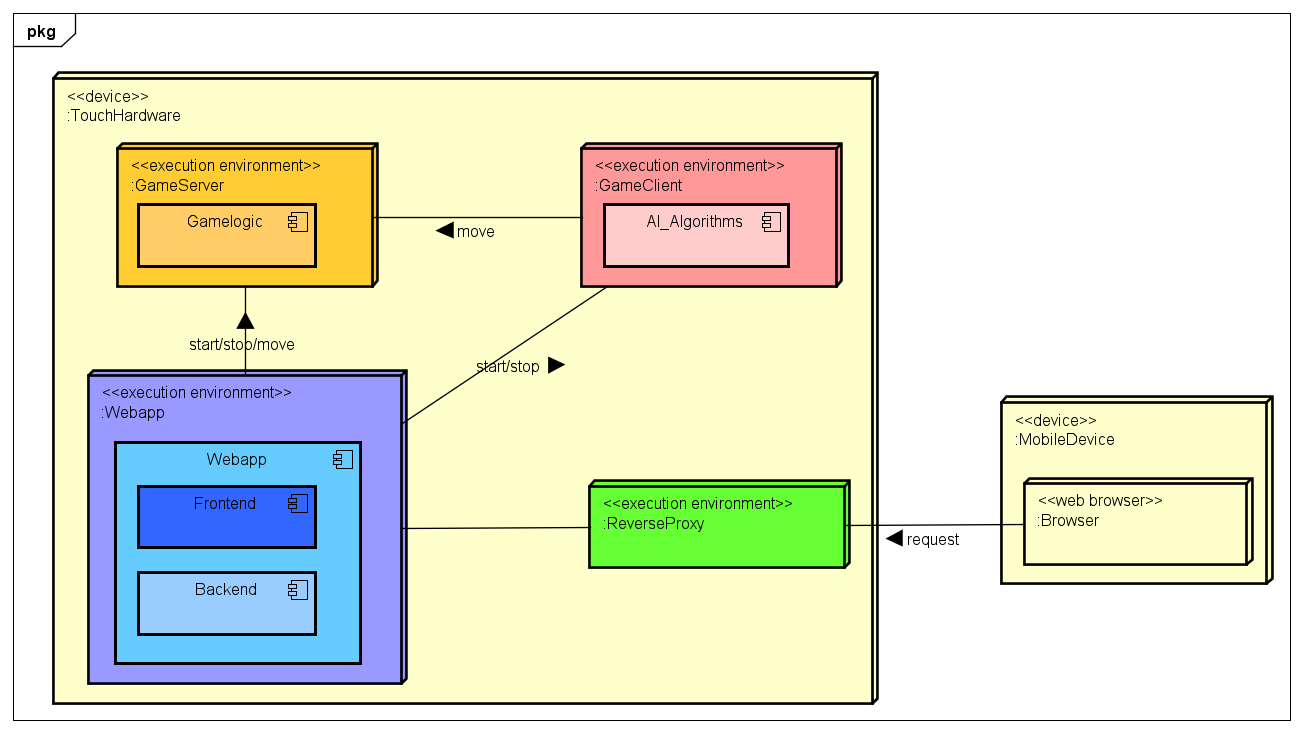
\includegraphics[width=1.0\linewidth]{pics/DeploymentDiagram.png}
	\captionof{figure}{ Die Anwendung als Verteilungsdiagramm}
	\label{fig:DeploymentDiagram}
\end{minipage}

\subsection{Gameserver}
Als Gameserver wird der Teil der Software betrachtet, welcher für das Einhalten der Spielregeln und die Verwaltung des Spielfeldzustandes 
verantwortlich ist. 

\subsubsection{Softwareaufbau des Gameservers}
Die Software des Gameservers ist in zwei Pakete aufgeteilt. Und zwar in das \texttt{Gamerulebook}- und das \texttt{Serverconnection}-Paket.
Der \texttt{Serverconnection} Teil ist für die Verbindung und das Decodieren der Nachrichten der Clients verantwortlich, siehe Abbildung \ref{fig:GameServerClassDiagram}.
Nachdem ein Client verbunden ist und seine Nachricht schickt, wird diese decodiert und falls das Protokoll korrekt eingehalten wird,
an den \texttt{Gamerulebook} Teil weitergeleitet. Das \texttt{Gamerulebook} Paket verwaltet den Spielzustand sowie die Spielregeln des laufenden Spieles.
Das Spielfeld wird in \texttt{GameStatus} gespeichert und bei neu eintreffenden Nachrichten mit neuen Zügen mit diesen aktualisiert.
Bevor ein neu eingetroffener Zug das Spielfeld aktualisiert, wird er erst über die Realisierungen des \texttt{GameRules} Interface überprüft.
Diese Realisierungen sind im Diagramm durch die Spiele Dame und Mühle dargestellt und befinden sich in den Paketen \texttt{Checkers} und \texttt{NineMensMorris}.
Über den weiteren Inhalt des \texttt{Checkers} Paketes wird im Kapitel \ref{chap:Spiellogik} auf Seite \pageref{chap:Spiellogik} berichtet, da es 
redundant in der Applikation vorzufinden und auch für den Gameclient relevant ist.

\vspace{1em}
\begin{minipage}{\linewidth}
	\centering
	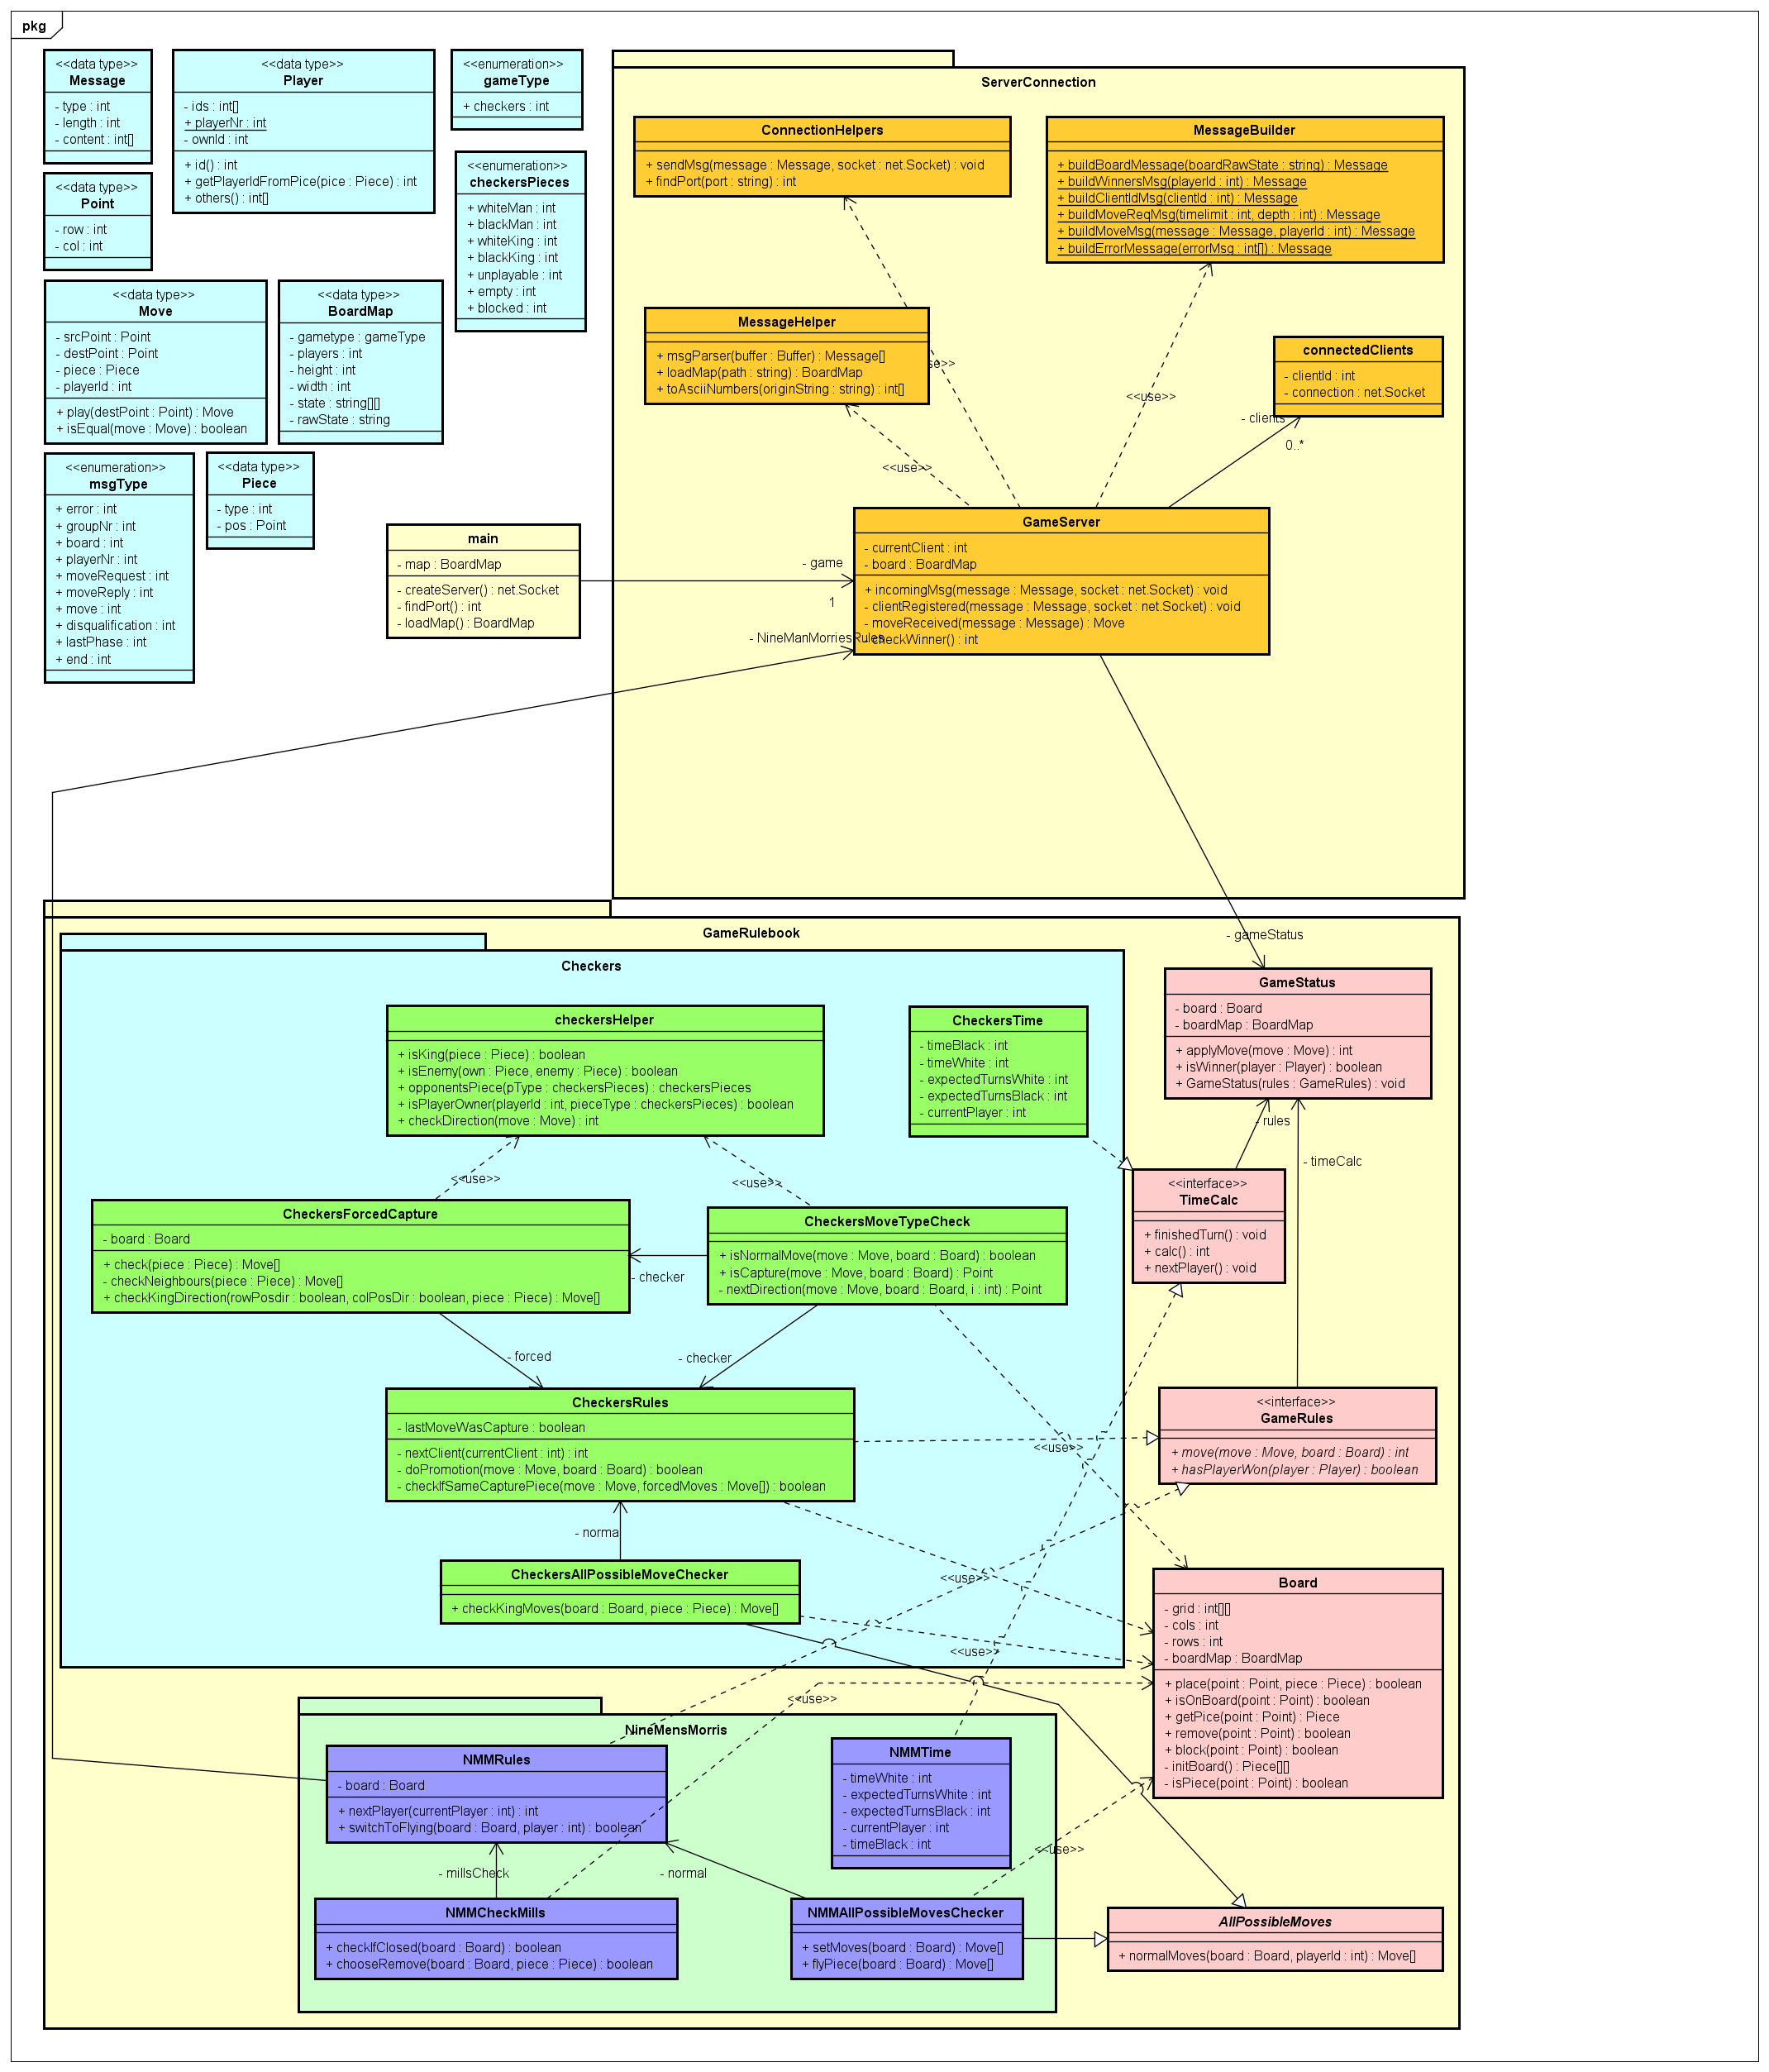
\includegraphics[width=1.0\linewidth]{pics/GameServerClassDiagram.png}
	\captionof{figure}{ Das \ac{UML} Klassendiagramm des Gameservers }
	\label{fig:GameServerClassDiagram}
\end{minipage}

\subsubsection{Erweiterung um weitere Spiele}
Ein beliebiges Spiel kann mittels des Interfaces \texttt{GameRules} zur Anwendung hinzugefügt werden, was dem Gameserver die Eigenschaft gibt, um 
beliebig viele Spiele erweiterbar zu sein, siehe Abbildung \ref{fig:GameServerClassDiagram}. Welche Implementierung des Interfaces gewählt wird, 
wählt der Server anhand der Spielkarte, die an ihn
als Übergabeparameter übermittelt wird, aus. Wird ein neuer Zug registriert, werden abhängig vom Spiel die jeweils implementierten Methoden 
\texttt{move} und \texttt{hasPlayerWon} aufgerufen.
Die \texttt{move} Methode übernimmt die Validierung und Aktualisierung des Zuges am Spielbrett und
die \texttt{hasPlayerWon} Methode wird verwendet, um zu prüfen, ob die Voraussetzungen eines Spielendes erfüllt sind.
Klassen wie \texttt{Board} und \texttt{Move} sind vom Spieltyp unabhängig. Es muss nur ein bestimmter Typ (wie z. B. \texttt{checkersPieces}) für die \texttt{Piece} 
Klasse gewählt werden, um die Spielfiguren auf dem Spielfeld zu repräsentieren.  


\subsubsection{Server Kommunikation}
Für die Kommunikation des Servers ist das zuvor erwähnte Paket \texttt{Serverconnection} (Abbildung \ref{fig:GameServerClassDiagram}) verantwortlich.
Der Ablauf einer Verbindung eines Spieles mit zwei Spielern ist in Abbildung \ref{fig:SequenceDiagramGameServer} dargestellt. 
Dieser Ablauf ist unabhängig von der Art des Spieles und immer, also sowohl für Dame als auch Mühle, gleich.
Die beiden dargestellten Clients, \texttt{Client1} und \texttt{Client2} können zwei beliebige Applikationen sein, welche über dasselbe Protokoll
wie der Gameserver kommunizieren.
\\
Nachdem der Gameserver gestartet wird, geht er sofort, in den Wartemodus über. Dabei wartet er, bis sich irgendjemand
mit seinem Port verbindet. Sobald die geforderte Anzahl an Spielern für ein gewähltes Spiel mit \texttt{register} 
verbunden ist, wie im Beispielfall der Abbildung \ref{fig:SequenceDiagramGameServer}, 
startet er ein neues Spiel und sendet die Zugaufforderung \texttt{moveRequest} 
an den Spieler, der sich zuerst registriert hat. Kommt eine Nachricht mit einer Zugantwort zurück,
wird der nächste Spieler benachrichtigt, der an der Reihe ist. Dieser Ablauf wird bis zum Spielende wiederholt, wobei die Spieler mittels \texttt{gameResult}
über das Resultat des Spieles informiert werden.
\\


\vspace{1em}
\begin{minipage}{\linewidth}
	\centering
	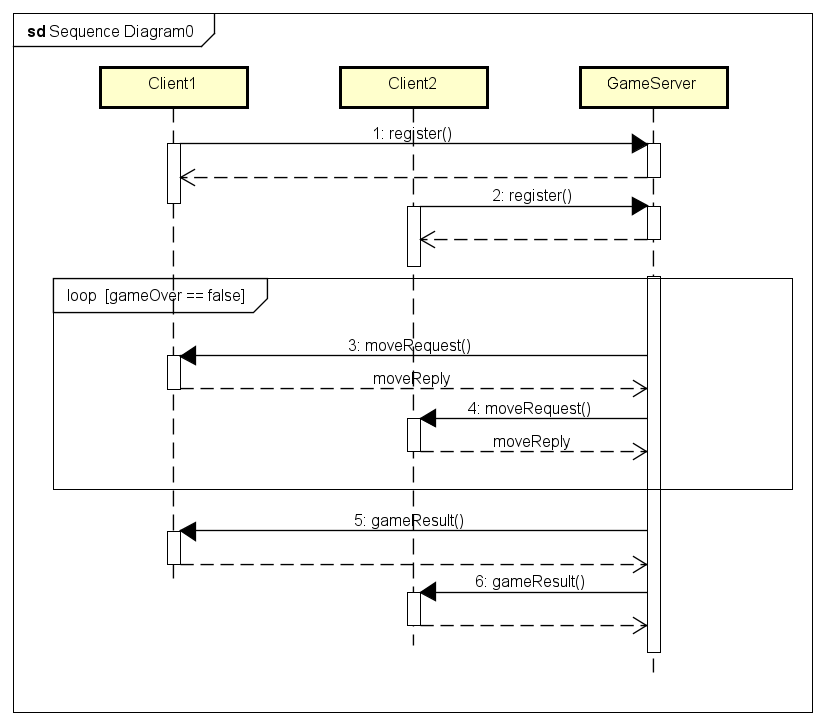
\includegraphics[width=0.7\linewidth]{pics/SequenceDiagramGameServer.png}
	\captionof{figure}{ Das Sequenzdiagramm zum Ablauf der Serververbindung }
	\label{fig:SequenceDiagramGameServer}
\end{minipage}


\subsubsection{Zeitlimits für Spieler}
\label{chap:timelimit}
Da in vielen Brettspielen, die auf Wettkampfbasis betrieben werden, Zeituhren verwendet werden, gibt es auch ein Interface \texttt{TimeCalc}, das
für die Zeitüberprüfung der Clients verwendet wird, siehe Abbildung \ref{fig:GameServerClassDiagram} auf Seite \pageref{fig:GameServerClassDiagram}. 
Vor allem bei künstlichen Intelligenzen ist eine Zeitüberprüfung notwendig, weil ein 
Zeitlimitverzicht zu einer sehr langen Berechnungsdauer führen kann. So kann es sein, dass ein Algorithmus wie Minimax, mit einer Suchtiefe von 7, bei einfachen
Stellungen nur wenige Sekunden braucht, aber bei weitaus komplexeren Stellungen mehrere Stunden. 
Das \texttt{TimeCalc} Interface behandelt zwei Fälle, nämlich den Spielverlust auf Zeit und die 
Dauer, die eine \ac{KI} für den nächsten Zug brauchen soll. Der Spielverlust auf Zeit ist relativ einfach erklärt. Braucht ein Teilnehmer länger als 
die vorgesehene Zeit, verliert er das Spiel. Die berechnete Dauer des nächsten Zuges der \ac{KI} gibt an, wieviel Zeit die \ac{KI} zur Verfügung hat, um ein
Ergebnis zu liefern und soll anhand dieser für den jeweiligen Spieltyp über das 
Interface \texttt{TimeCalc} implementiert werden. Damit kann anhand der Spielsituation dem nächsten Zug mehr oder weniger Zeit zugewiesen werden. 
Zum Beispiel könnte man einer \ac{KI} in der Eröffnungphase mehr und zum Spielende hin weniger Zeit geben. 
Die Entscheidung, die Berechnung der \ac{KI}-Zeit im \texttt{GameServer} und nicht im \texttt{GameClient} auszuführen, basiert zum einen darauf, 
dass die gesamte Zeitberechnung im Server zusammengefasst ist und zum anderen, dass
die Zeitberechnung eines schon implementieren Spieles verwendet werden kann, wenn die Applikation um ein Spiel erweitert wird.

\subsection{Webapp}

\vspace{1em}
\begin{minipage}{\linewidth}
	\centering
	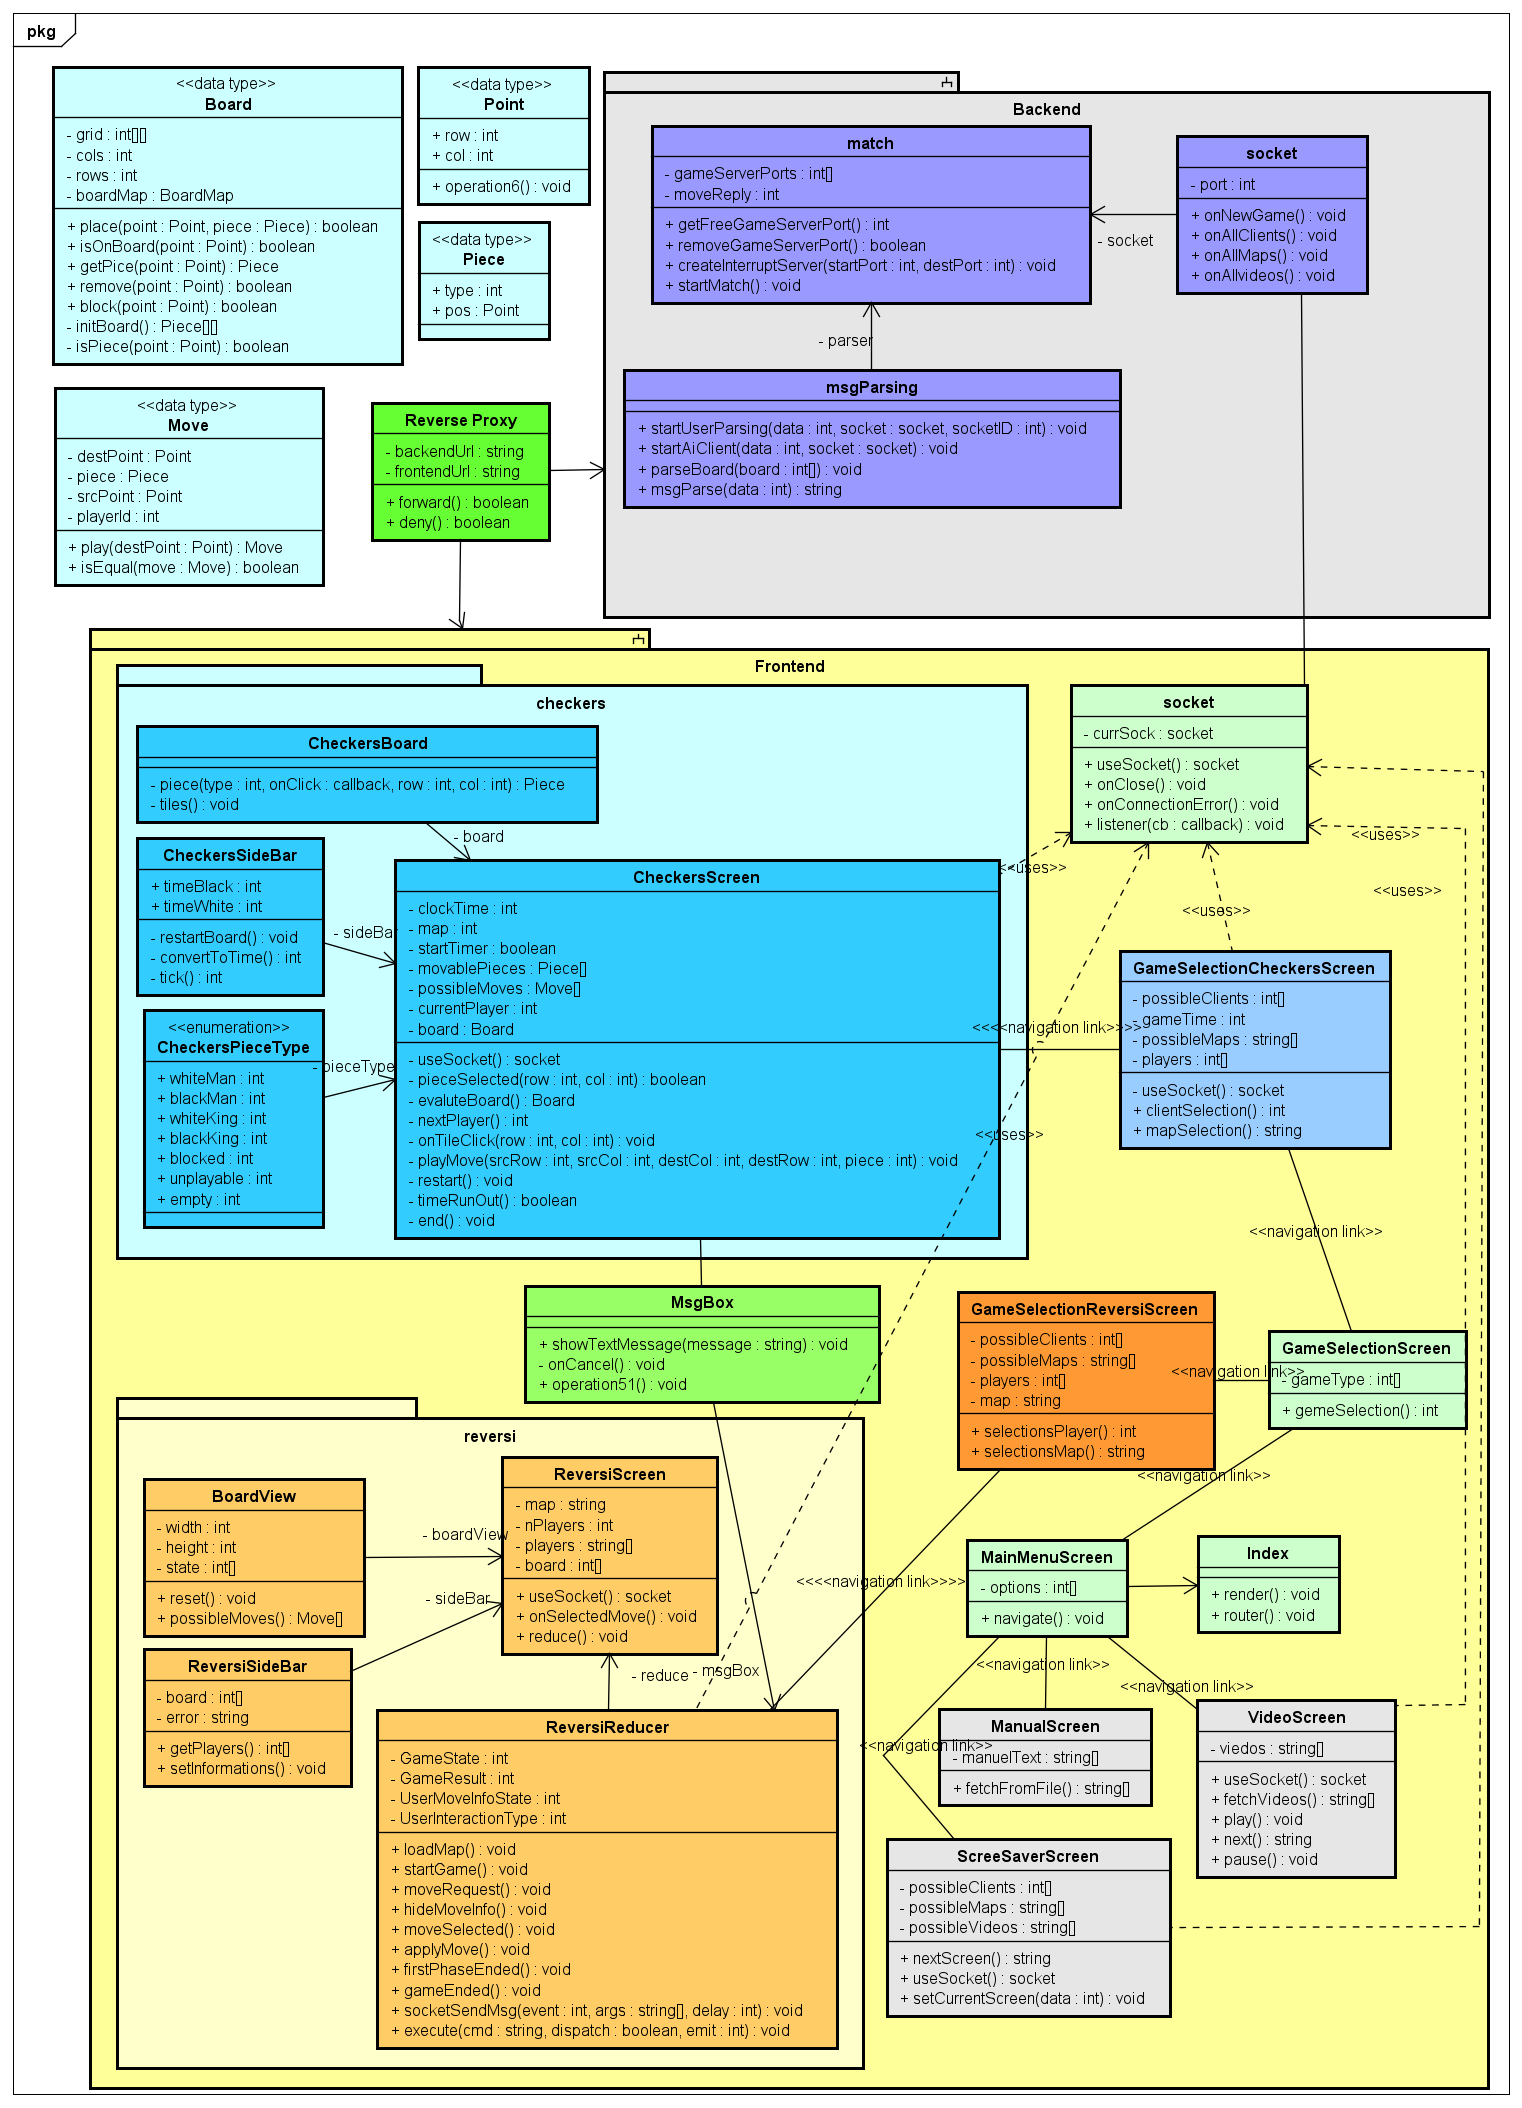
\includegraphics[width=0.9\linewidth]{pics/ReversiXTGUIClassDiagramm.png}
	\captionof{figure}{ Das \ac{UML} Klassendiagramm der \ac{ReversiXT} \ac{GUI} }
	\label{fig:ReversiXTGUIClassDiagram}
\end{minipage}
\\

Die Webapp ist der Teil der Software, der für die eigentliche Benutzerinteraktion verwendet wird. Benutzer können über die \ac{GUI}
Spiele starten, bei welchen sie gegen KIs oder andere User spielen können. Dabei setzt sich die Webapp aus einem Frontend und 
einem Backend zusammen, siehe Abbildung \ref{fig:ReversiXTGUIClassDiagram}. 
Das Frontend wird zur Darstellung der graphischen Oberfläche der Anwendung verwendet. Über die Interaktion mit der 
\ac{GUI} können Benutzer ein Spiel auswählen und Einstellungen treffen, welche die Spielregeln des Spieles verändern.
Beim Start eines Spiels, wird ein Spielfeld mit Zugmöglichkeiten geboten, welche es dem Benutzer erlauben 
Züge auszuführen.
Diese ausgewählten Optionen und Züge werden an das Backend weitergeleitet, die den Gameserver und den Gameclient 
startet und diese über die Aktionen des Benutzers an der \ac{GUI} informiert. 

\subsubsection{Frontend}
Das Frontend, in Abbildung \ref{fig:ReversiXTGUIClassDiagram} als gelbes Paket gekennzeichnet, ist, wie schon zuvor erwähnt die
\ac{GUI} Komponente der gesamten Anwendung. Da die Aufgabe dieses Projektes die Erweiterung der Software um das Spiel Dame ist, 
wird die Struktur des Frontendes übernommen und durch weitere Menüs sowie dem Spielfeld erweitert. Dabei bleibt der vorhandene Teil der Software gleich 
und wird aus Sicht der Architektur nicht weiter beschrieben. 
\\
Die erste Veränderung ist das Einbauen eines neuen Menüs, über welches das Spiel ausgewählt werden kann. In Abbildung \ref{fig:ReversiXTGUIClassDiagram} 
handelt es sich hierbei um die Klasse \texttt{GameSelectionScreen}. Vorher wurde über den Menübutton ``Spielen'' direkt das Auswahlmenü \texttt{GameSelectionReversiScreen}
(siehe Abbildung \ref{fig:ReversiMenu} und \ref{fig:ReversiGameSelection} auf Seite \pageref{fig:ReversiMenu}) zum Konfigurieren eines Reversi Spieles erreicht. 
Nun soll der \texttt{GameSelectionScreen} davor geschaltet sein. Dieses weitere Menü beinhaltet nun Möglichkeiten der Navigation zu allen weiteren Spielen.
Würde man das Projekt um ein weiteres Spiel erweitern wollen, so müsste man lediglich eine weitere Option zum \texttt{GameSelectionScreen} hinzufügen 
und der eigentliche Spielfeldaufbau und Spielfluss kann in ein weiteres eigenes Paket hinzugefügt werden, welches nur über dieses Menü erreichbar ist.
\\
Um das Spiel Dame konfigurieren zu können, also ob Benutzer oder \ac{KI} antreten soll, und welche auf welcher Karte gespielt wird, gibt es ein eigenes Menü, 
in dem diese Einstellungen vorgenommen werden können. \texttt{GameSelectionCheckersScreen} beschreibt genau dieses Menü und bietet die Schnittstellen 
zum \texttt{Checkers} Paket, welches die Darstellung des eigentlichen Spieles beinhaltet. Wichtig ist hier noch zu erwähnen, dass das \texttt{GameSelectionCheckersScreen}
Menü über die \texttt{Socket} Klasse direkten Zugriff auf das Backend hat. Über diesen Zugriff werden, nachdem alle Einstellungen getroffen sind und ein Spiel
gestartet wird, jeweils die anderen Komponenten der Software, wie Gameserver und Gameclient, gestartet. In Kapitel \ref{chap:NetworkModie} auf Seite \pageref{chap:NetworkModie} 
wird nochmal genauer darauf eingegangen, welche Komponente gestartet wird.
\\
Das Paket \texttt{Checkers} setzt sich aus dem \texttt{CheckersBoard}, dem eigentlichen Spielfeld, und der \texttt{CheckersSideBar}, den Informationen zum laufenden Spiel, zusammen. 
Das \texttt{CheckersBoard} ist abhängig von der gewählten Karte und passt seine Form und Größe der Karte an. Jeder Zug, der auf dem Spielfeld ausgeführt wird, muss an 
die \texttt{CheckersScreen} Klasse geschickt werden, welche dann die Informationen ans Backend weitergibt.
Die \texttt{CheckersSideBar} verwaltet Informationen wie Zeitlimits und Spielerfarben. 
Ist ein Spiel zu Ende, oder ein Fehler tritt auf, wird die Klasse \texttt{MsgBox} benötigt. Über diese Klasse werden Spielinformationen, welche das Spiel beenden, 
dargestellt.

\subsubsection{Backend}
Das Backend, in Abbildung \ref{fig:ReversiXTGUIClassDiagram} als graues Paket dargestellt, verwaltet die Kommunikation zu den anderen Komponenten der Anwendung.
Es ist eine eigene Anwendung, welche parallel zum Frontend läuft und mit diesem über seine \texttt{socket} Klasse kommuniziert.
Die Besonderheit liegt hierbei auf der \texttt{match} Klasse, die verwendet wird, um ein Spiel zu verwalten. 
Diese Klasse startet abhängig von der gewählten Einstellung von Gameserver und Gameclient und verbindet sich mit beiden. Das Kapitel \ref{chap:NetworkModie} auf 
Seite \pageref{chap:NetworkModie} erläutert dies im Detail. Spielzüge aus dem Frontend werden somit 
an den Gameserver weitergeleitet und Züge die von anderen Komponenten an den Gameserver geschickt wurden und von diesen angenommen sind, kommen zurück zum Frontend.
Da der Gameserver, der Gameclient und das Backend die gleiche Codierung benutzen müssen, um Nachrichten austauschen zu können, wird 
die Klasse \texttt{msgParsing} zum Dekodieren und Enkodieren der Nachrichten benötigt.

\subsubsection{Reverse Proxy}
Eine der Anforderungen ist, dass es für den Benutzer möglich sein muss, sich mit einem Mobilgerät mit der Software zu verbinden und als Spieler eine
Partie Dame spielen zu können. Diese Mobilverbindung muss Sicher gehalten werden, wodurch nur bestimmte Anfragen an die Anwendung durchgelassen werden.
In Abbildung \ref{fig:ReversiXTGUIClassDiagram} ist der Reverse Proxy in Grün dargestellt.
\\ 
Ein Reverse Proxy wird verwendet, um Anfragen an den Server weiterzuleiten und die geforderten Ressourcen an den Client zurückzuschicken. Dabei 
bleibt die wahre Adresse des Servers dem Client verborgen, weil dieser nur über den Reverse Proxy mit ihm kommunizieren kann.
Erhält der Proxy eine Anfrage, welche der Nutzer nicht stellen darf, so verweigert er den Zugriff auf den Server.
\\
Da die Architektur der Software für eine Webanwendung gedacht ist und der Nutzer extern mit seinem Mobilgerät auf die Website zugreift, 
muss dieser über diese Website auf das Backend der Webapp zugreifen, um Daten, wie Züge, holen zu können.
Über die Webanwendung am Server wird, immer wenn ein Spiel ausgewählt wird, ein Gameserver gestartet, somit könnte ein böswilliger Benutzer
mit einem selbstgeschriebenen Programm, welches das Protokoll des Servers einhält, beliebig viele Gameserver starten und damit die 
Anwendung zum Absturz bringen.
Der Proxy ist eine Absicherung, dass der Benutzer sich nicht direkt auf das Backend ohne Website verbinden und somit 
keinen Schaden anrichten kann. 

\subsection{Gameclient}
Der Gameclient beinhaltet die Logik der künstlichen Intelligenz der Applikation. Wird ein Spiel gegen einen Gameclient gewählt, so wird dieser gestartet und agiert als 
Gegenspieler zum User. Der User kann ebenso ein Spiel, bei welchem zwei \ac{KI}s gegeneinander spielen, starten. Dadurch werden zwei Clients aktiviert.
Da im Projekt mehrere verschiedene \ac{KI}-Algorithmen implementiert sind, ist hier ebenfalls eine modulare Architektur wichtig.

\subsubsection{Genereller Aufbau}
Der Gameclient besteht aus den drei Paketen \texttt{CheckersAiLogic}, \texttt{Checkers} und \texttt{Server}, siehe Abbildung \ref{fig:KIClientClassDiagram}. 
In \texttt{Checkers} befindet sich die Spiellogik, welche einen Momentanzustand des Spielbrettes sowie Möglichkeiten dieses nach Belieben zu modifizieren beinhaltet 
und ist in Kapitel \ref{chap:Spiellogik} genauer erklärt, da es sich um das gleiche, wie im Gameserver verwendete Paket, handelt. 
Für die Verbindung zum Gameserver wird das \texttt{Server}-Paket gebraucht, in dem eingehende und ausgehende Nachrichten übertragen werden.
Der Kern des Clients ist in \texttt{CheckersAiLogic}. Hier sind die Algorithmen, welche zur Berechnung von neuen Zügen 
benutzt werden.

\vspace{1em}
\begin{minipage}{\linewidth}
	\centering
	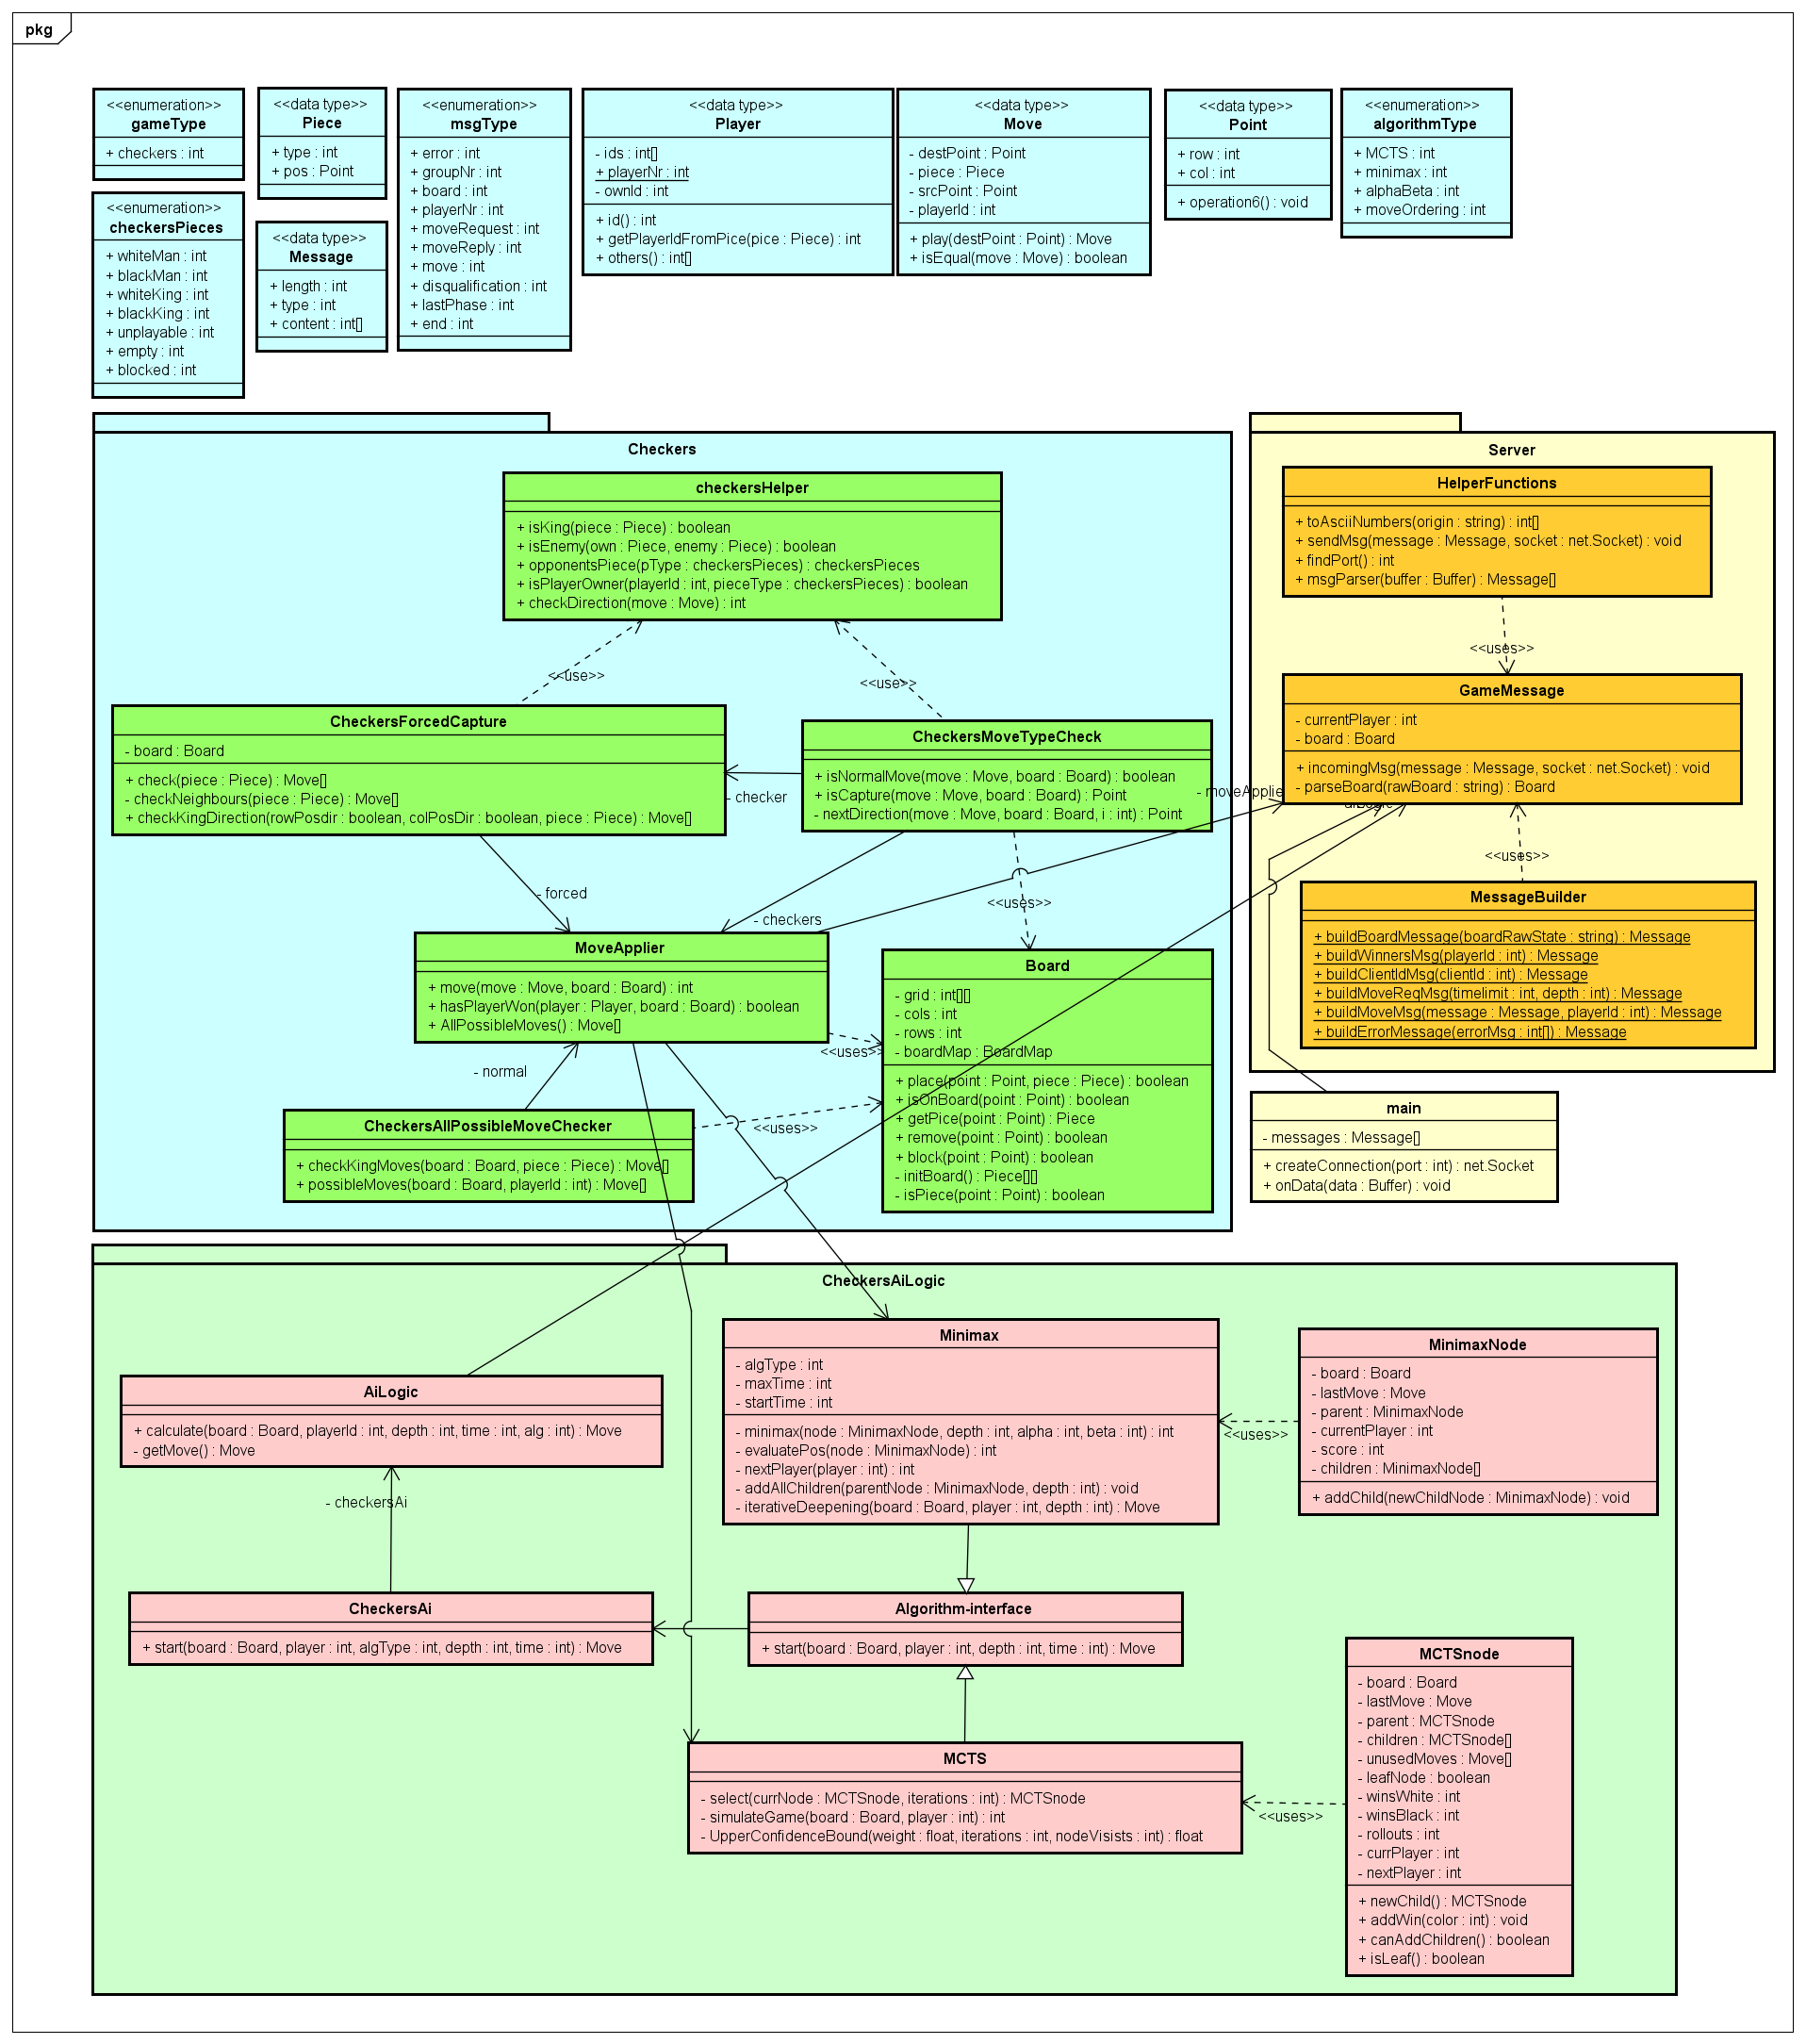
\includegraphics[width=0.9\linewidth]{pics/GameClientClassDiagram.png}
	\captionof{figure}{ Das \ac{UML} Klassendiagramm des \ac{KI} Clients }
	\label{fig:KIClientClassDiagram}
\end{minipage}

\subsubsection{\ac{KI} Logik}
In Abbildung \ref{fig:KIClientClassDiagram} erkennt man das in grün eingefärbte Paket \texttt{CheckersAiLogic}, welches für die \ac{KI} Logik der Applikation verantwortlich ist.
Jeder \ac{KI}-Algorithmus, der zur Applikation hinzugefügt wird, muss das \texttt{Algorithm-interface} implementieren. Die Methode \texttt{start} ist dabei für die Berechnung 
verantwortlich. Die Grundvoraussetzung, die dabei jeder Algorithmus bekommt, ist das Spielfeld, der Spieler der am Zug ist, die Tiefe und die Zeit, wie lange gesucht werden darf.
Als Ergebnis wird ein Zug erwartet, welcher aus Sicht der \ac{KI} der beste Zug in der jeweiligen Stellung ist. Dadurch ist es möglich, die Applikation durch beliebig weitere 
Algorithmen, wie Deep Learing, einfach zu erweitern. 
Viele \ac{KI}-Algorithmen brauchen, damit sie neue Stellungen evaluieren oder aus einer Stellung andere Stellungen simulieren können, eine Möglichkeit, um das Spielfeld mittels 
Zügen verändern zu können. Die Klasse \texttt{MoveApplier} aus dem \texttt{Checkers} Paket erreicht genau dieses Vorhaben, indem sie es erlaubt, Züge auf einem Spielfeld auszuführen 
sowie alle Züge, die aus einer Stellung heraus möglich sind, anzuzeigen.
\\
In der zuvor erwähnten Abbildung sind zwei dieser Algorithmen zu sehen. Dabei handelt es sich um Minimax und \ac{MCTS}. Da diese beiden Algorithmen zu den Baum-Algorithmen
gehören, haben beide ihre ``Node''-Klassen. Dabei ist die Klasse eine Beschreibung der Knoten des Baumes, der im Laufe der Berechnung aufgebaut wird.
Zur Auswahl der Algorithmen findet man die Klasse \texttt{AiLogic} vor, die eine Auswahl der verschiedenen Algorithmen bietet. 
\\ 
Die Besonderheiten dieses Paketes befinden sich in der Implementierung, welche in einem späteren Kapitel genauer erläutert wird 
(Kapitel \ref{chap:KIAlgorithms} auf Seite \pageref{chap:KIAlgorithms}).

\subsubsection{Verbindung zum Server}
Das Paket \texttt{Server} aus Abbildung \ref{fig:KIClientClassDiagram} ist zur Verbindung mit dem Gameserver gedacht, dabei verwendet es das vom Gameserver geforderte 
Protokoll. Die genauen Details des Protokolles werden durch die Klasse \texttt{MessageBuilder} versteckt, welches statische Methoden anbietet Nachrichten zu generieren.
\texttt{GameMessage} ist die zentrale Komponente zur Kommunikation, hier werden Nachrichten enkodiert und dekodiert und je nach Nachrichteninhalt 
Züge mittels des \texttt{CheckersAiLogic} Paket generiert.

\subsection{Dame Spiellogik}
\label{chap:Spiellogik}
Die Spiellogik für Dame ist mehrfach in der Anwendung vorfindbar. Zum einen, um Züge im \ac{KI}-Client zu testen und zum anderen
für den Gameserver zur Überprüfung und Aktualisierung der Züge. In den Abbildungen \ref{fig:KIClientClassDiagram} und \ref{fig:GameServerClassDiagram} 
auf der Seite \pageref{fig:KIClientClassDiagram} bzw. \pageref{fig:GameServerClassDiagram}
befindet sich die Spiellogik im Paket \texttt{Checkers}. Diese Redundanz ist wichtig, da es sich beim Server und Client um eigenständige Prozesse handelt 
und diese nicht die gleiche Code-Basis haben. Eine Möglichkeit diese Redundanz zu vermeiden wäre, die Validierung in den Gameserver zu verschieben und 
den Gameclient zu zwingen, dass jeder Zug vom Gameserver validiert werden muss. Dies erhöht aber die Netzwerkkommunikation und verlangsamt das Finden eines Zuges 
durch den daraus entstehenden Overhead.
\\
Die Abbildung \ref{fig:GameLogic} zeigt die Spiellogik vom Paket \texttt{Checkers} unabhängig von der Applikation, in der es verwendet wird.
Die Hauptklassen der Spiellogik sind die \texttt{Board}-, \texttt{Move}- und \texttt{Player}-Klasse. Dabei hält die \texttt{Board}-Klasse die Information über das aktuelle Spielbrett sowie 
Methoden um Spielsteine auf dem Spielbrett zu entfernen oder zu bewegen. 
Die \texttt{Move}-Klasse dient zum Repräsentieren eines Zuges. Sie besteht aus dem 
Ursprungspunkt, dem Zielpunkt, dem Spieler, der den Zug getätigt hat und um welchen Spielstein es sich handelt. 
\\
Die Klassen \texttt{CheckersForceCapture} und \texttt{CheckersAllPossibleMovesChecker} sind Klassen zum Finden aller möglichen Züge, die aus einer Stellung heraus gespielt werden
können. Dabei ist \texttt{CheckersForceCapture} verantwortlich für Züge, bei denen ein Spieler gezwungen wird, eine Figur zu schlagen und \texttt{CheckersAllPossibleMovesChecker} 
für alle Züge die keinen Schlagzwang haben. Die Aufteilung in zwei Klassen hat folgenden Hintergrund: Falls es sich um einen Schlagzwang handelt, besteht keine Notwendigkeit 
die \texttt{CheckersAllPossibleMoves}-Klasse zu erzeugen, welche Züge zu findet. Damit einen von der Netzwerkkommunikation eingehenden Zug zu überprüfen, 
werden die Methoden der \texttt{CheckersMoveTypeCheck}-Klasse verwendet. Sie vergleichen einen gegebenen Zug, 
den zum Beispiel der Benutzer getätigt hat, mit den Zügen die aus \texttt{CheckersForceCapture} und \texttt{CheckersAllPossibleMovesChecker}
hervorgehen. Dieses Vergleichen ist sehr wichtig für den Gameserver, da alle Züge, die von den Clients kommen, valide sein müssen. Im Gameclient wird das Vergleichen nur 
als Extra-Validierung verwendet, um den gesendeten Zug aus dem Gameserver nochmal zu überprüfen und so Fehler zu minimieren.
\\

\vspace{1em}
\begin{minipage}{\linewidth}
	\centering
	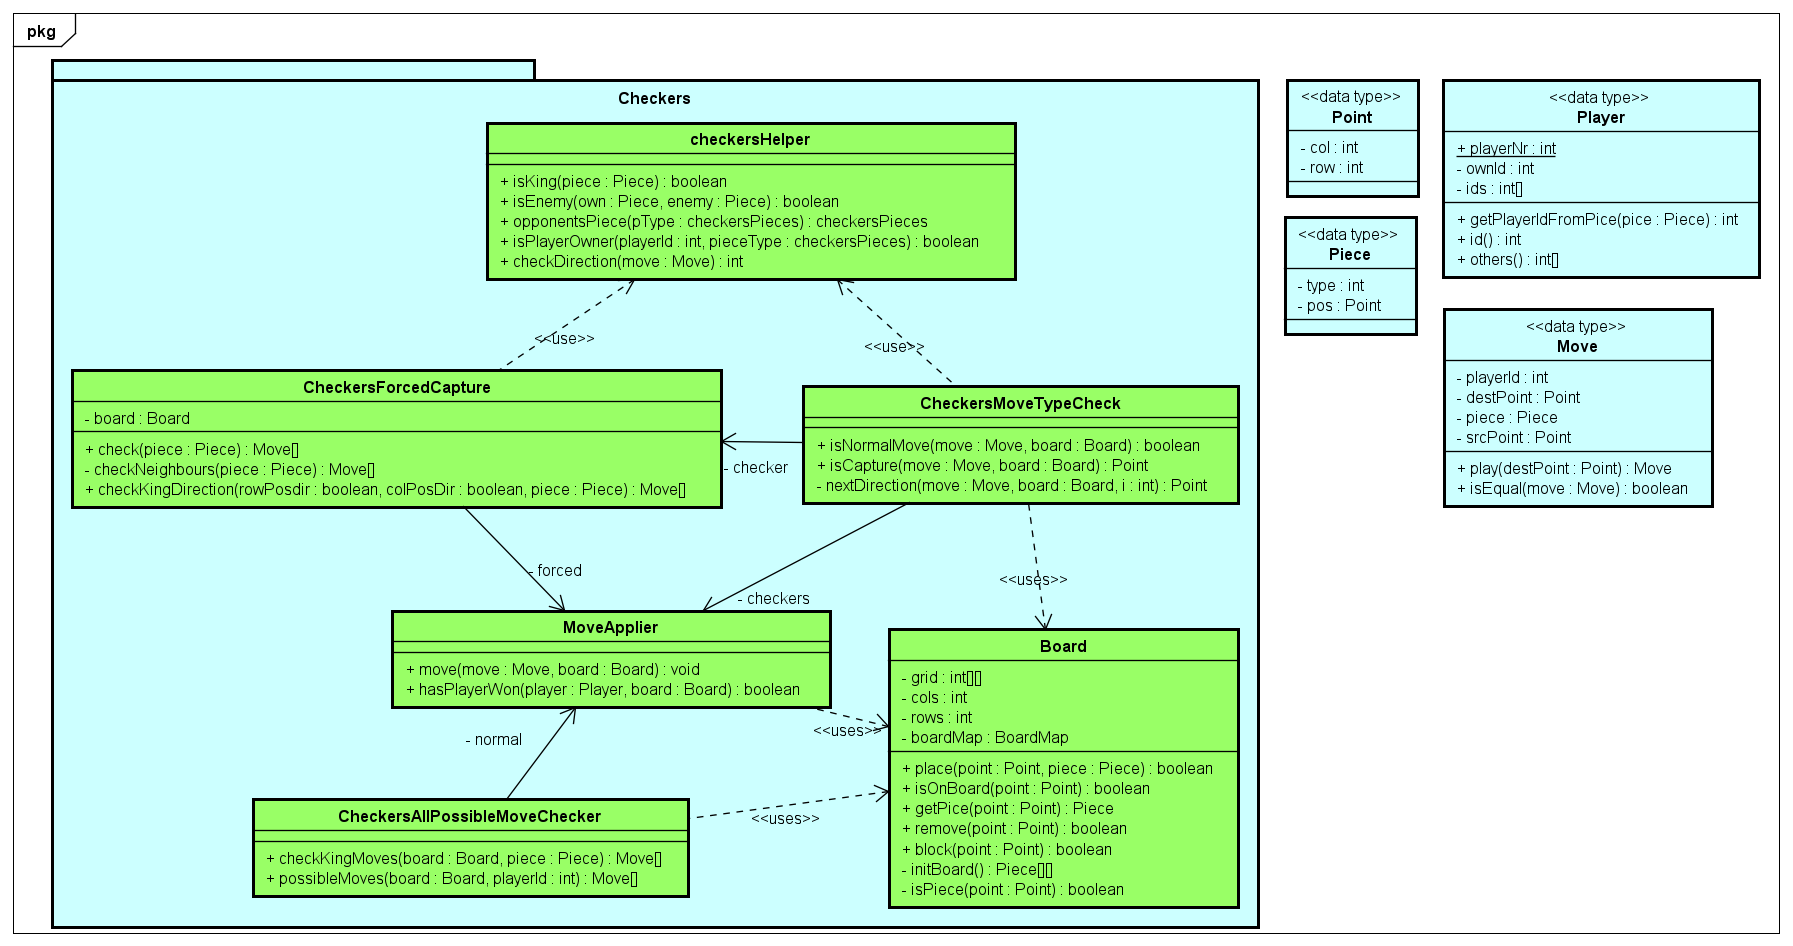
\includegraphics[width=1.0\linewidth]{pics/GameLogic.png}
	\captionof{figure}{ Das Paket Checkers, welches die Spiellogik beeinhaltet }
	\label{fig:GameLogic}
\end{minipage}



\subsection{Netzwerkkommunikation}
\label{chap:Networkcom}
Durch das Aufteilen der Anwendung in mehrere ausführbare Programme teilen sich die Programme keinen gemeinsamen Quellcode und laufen parallel zueinander. 
Dies hat zur Folge, dass eine Netzwerkkommunikation zwischen den Programmen erforderlich ist, um den Ablauf zu regulieren.

\subsubsection{Kommunikation zwischen den Software-Teilen}
Die Kommunikation zwischen den drei Anwendungen ist in Abbildung \ref{fig:ComponentDiagram} auf Seite \pageref{fig:ComponentDiagram} als 
Komponentendiagramm dargestellt. Dabei ist die gelbe Komponente der Gameserver, die blaue die Webapp, die rote der Gameclient und die grüne der Reverse Proxy.
Der dunkelblaue Teil der Webapp beinhaltet das Frontend, also die graphische Oberfläche der Anwendung.
Die hellblauen Komponenten beschreiben das Backend. 

In der Kommunikation zwischen dem Backend und dem Frontend der Webapp Komponente, werden Züge über das \texttt{incomingMove} Interface des Backends an das Frontend
weitergereicht. Züge, die von der graphischen Oberfläche aus gespielt werden, kommen über das Interface \texttt{sendInstructions} an das Backend. Dieses
Interface wird außerdem verwendet, um Befehle wie starten und stoppen eines Spieles zu übermitteln. Die Webapp Komponente hat zwei Ports nach außen, 
welche Nachrichten an das Backend
weiterreichen. Der erste Port übernimmt alle Nachrichten, die mit Zügen in Verbindung stehen. So werden alle Züge, die der Gameserver annimmt
und als Broadcast an alle Teilnehmer weitergibt, über diesen Port übertragen. Weitere Züge aus dem Frontend werden ebenfalls über diesen Port gesendet.
Der zweite Port übernimmt das Starten und Stoppen des Gameservers und des Gameclients. 
Neben den oben genannten Verbindungen des Gameservers, hat dieser außerdem eine Verbindung zum Gameclient. Über diese Verbindung werden Züge, die von der 
\ac{KI} des Gameclients berechnet werden, an den Gameserver gesendet.

Will sich ein Smartphone mit der Anwendung verbinden, werden alle Anfragen an Frontend oder Backend der Webapp vom Reverse Proxy abgefangen und 
nach Überprüfung an diese Schnittstellen weitergegeben.


\vspace{1em}
\begin{minipage}{\linewidth}
	\centering
	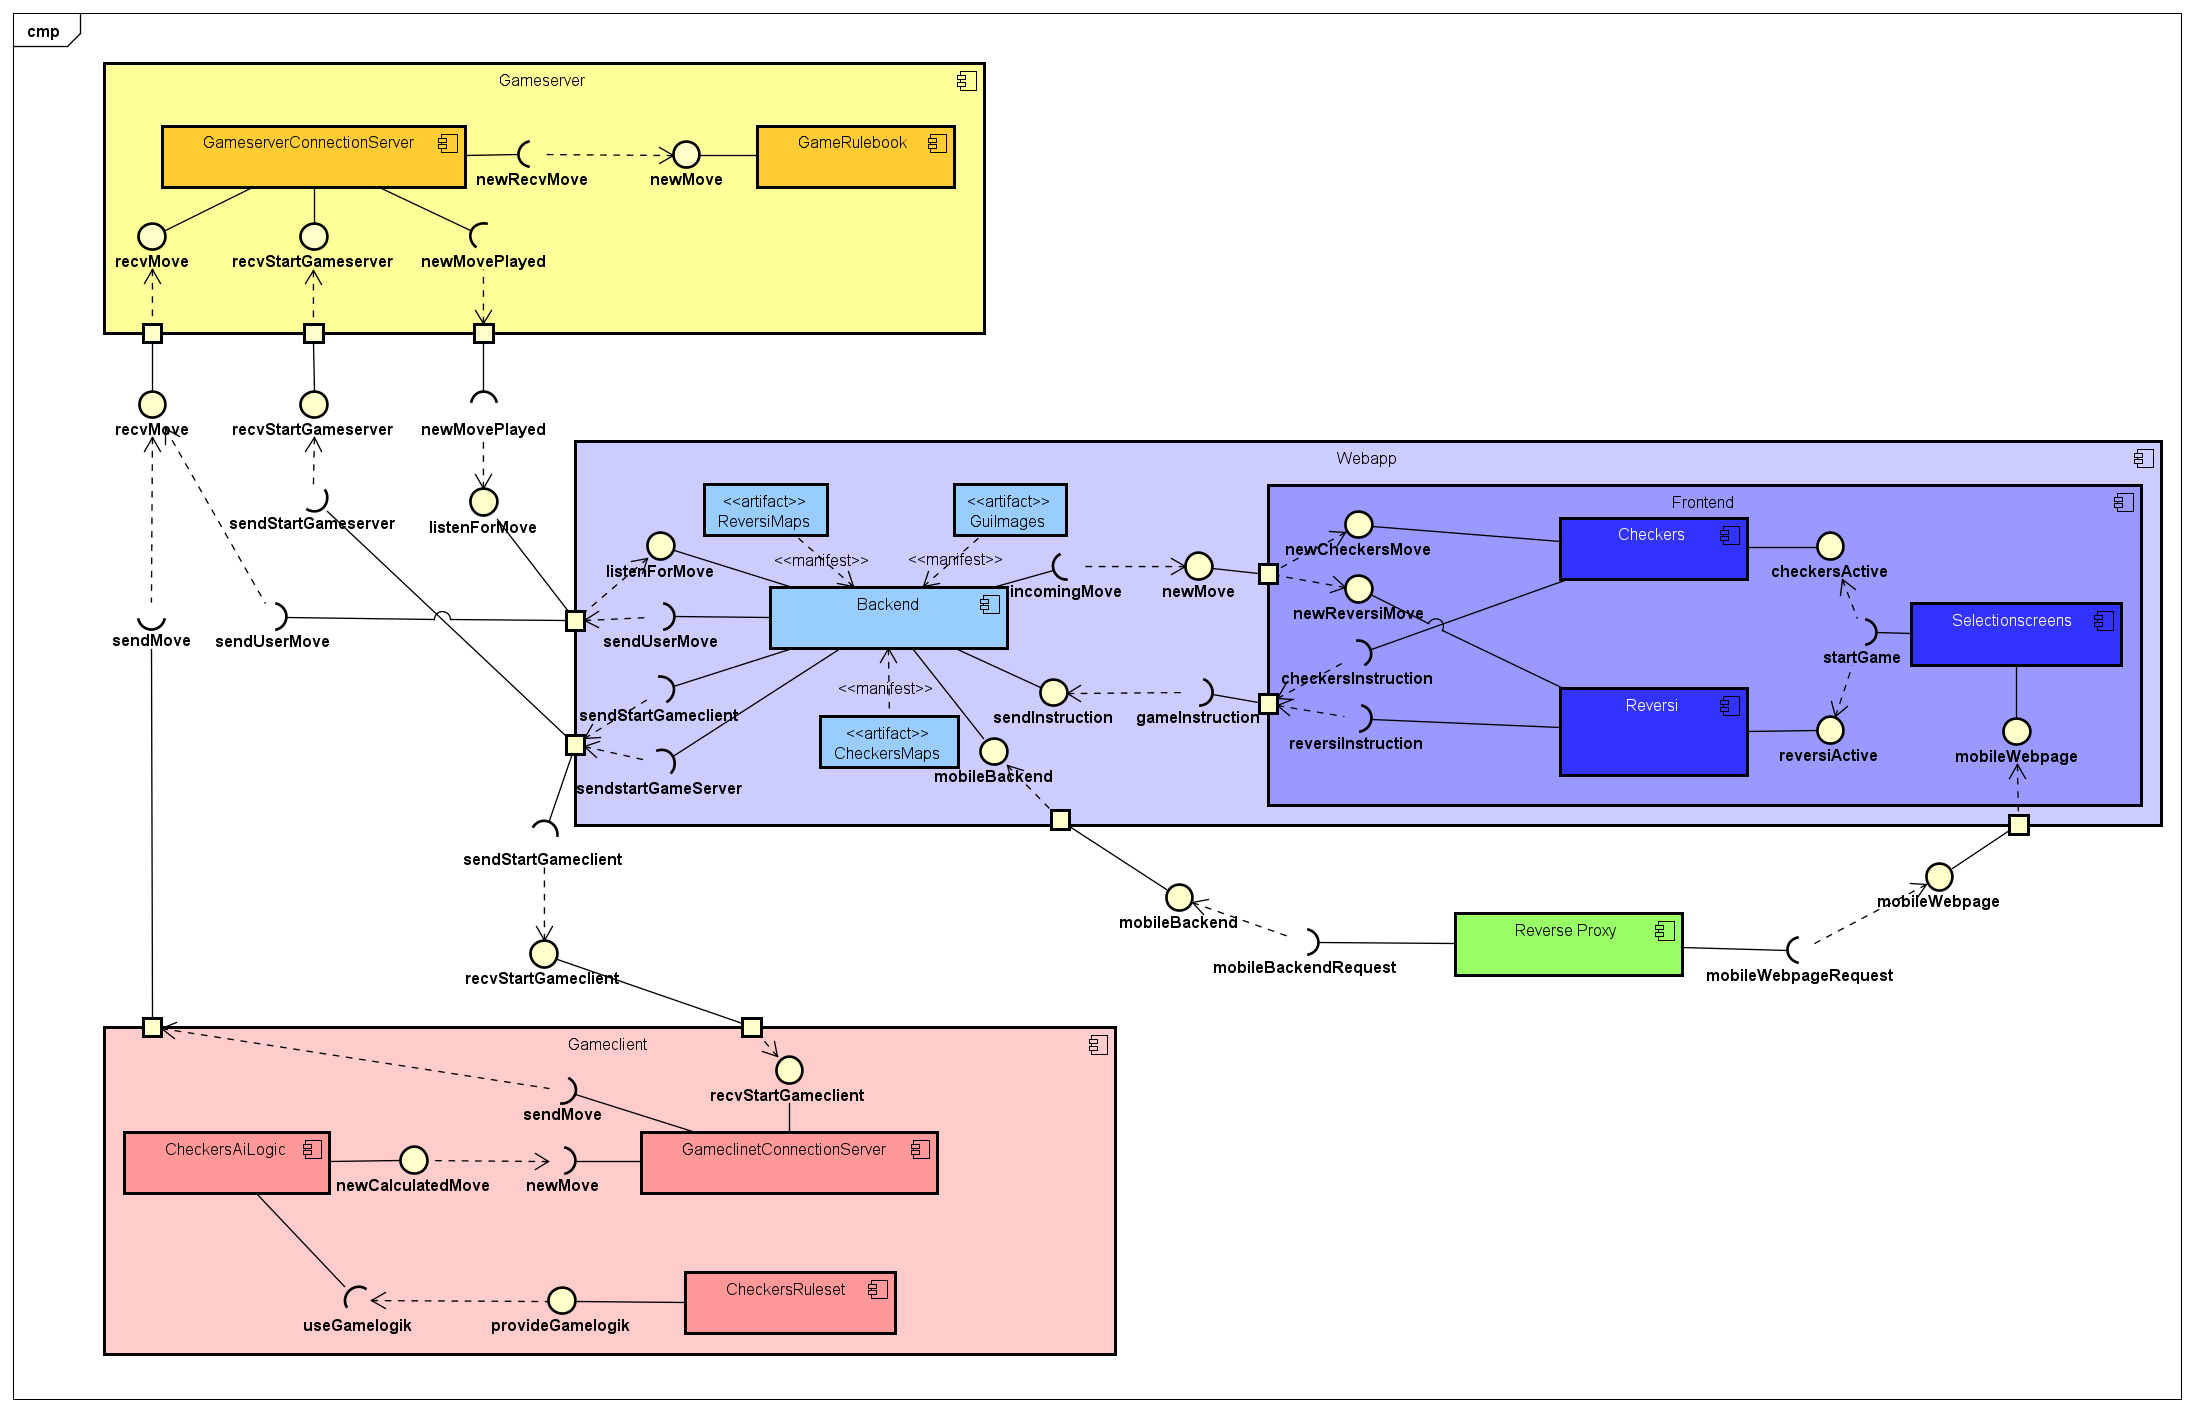
\includegraphics[width=1.0\linewidth]{pics/Komponentendiagram.png}
	\captionof{figure}{ Die gesamte Anwendung im \ac{UML} Komponentendiagram}
	\label{fig:ComponentDiagram}
\end{minipage}



\subsubsection{Kommunikation abhängig vom gewählten Spielmodus}
\label{chap:NetworkModie}
Da die Applikation mit mehreren Spielmodi ausgestattet ist, ändert sich die Kommunikation und welche Komponente gestartet werden muss, abhängig vom Modus.
Dabei werden die einzelnen Softwarekomponenten mit, je nach Modus, unterschiedlichen Parametern gestartet (für Details zu den Parametern, siehe Anhang \ref{apx:Parameters}
auf Seite \pageref{apx:Parameters}).
Die verfügbaren Spielmodi sind:
\begin{itemize}
    \item Benutzer gegen Benutzer
    \item Benutzer gegen \ac{KI}
    \item \ac{KI} gegen \ac{KI}
\end{itemize}
Unabhängig davon welche Option gewählt wird, wird der Gameserver immer gestartet, da dieser die Züge überprüft und Sieg oder Niederlage auswertet.
Bei Benutzer gegen Benutzer wird die \ac{KI}-Komponente der Software nicht ausgeführt. Die Webapp kommuniziert direkt mit dem Gameserver.
Wird sich für zwei Gameclients, die gegeneinander spielen entschieden, werden auch zwei gestartet.
Die Kommunikation findet nur noch zwischen dem Gameserver und den beiden Gameclients statt, jedoch hat die Webapp eine Man-in-the-Middle-Funktion,
wodurch sie die Kommunikation abhört und die gespielten Züge darstellen kann.
Das Spiel ``\ac{KI} gegen Benutzer'' ist das Szenario, das den größten Nutzen hat, da es am öftesten von den Benutzern gespielt wird.

Abbildung \ref{fig:UserVsUserSequenceDiagram} stellt ein \ac{UML} Sequenzdiagramm dar, bei welchem ein Benutzer gegen die \ac{KI} spielt.
Zuerst startet der Benutzer über die \ac{GUI} mit dem Spielmodus ein Spiel. Dadurch wird der Gameserver sowie ein
Gameclient ausgeführt. Würde man stattdessen \ac{KI} gegen \ac{KI} als Parameter mitsenden, würden zwei Gameclients gestartet. 
Der Gameserver wartet, bis sich zwei Spieler registriert haben. Ist die Registrierung abgeschlossen, werden
abwechselnd Züge von den Clients angefordert, bis ein Spieler gewonnen hat.

\vspace{1em}
\begin{minipage}{\linewidth}
	\centering
	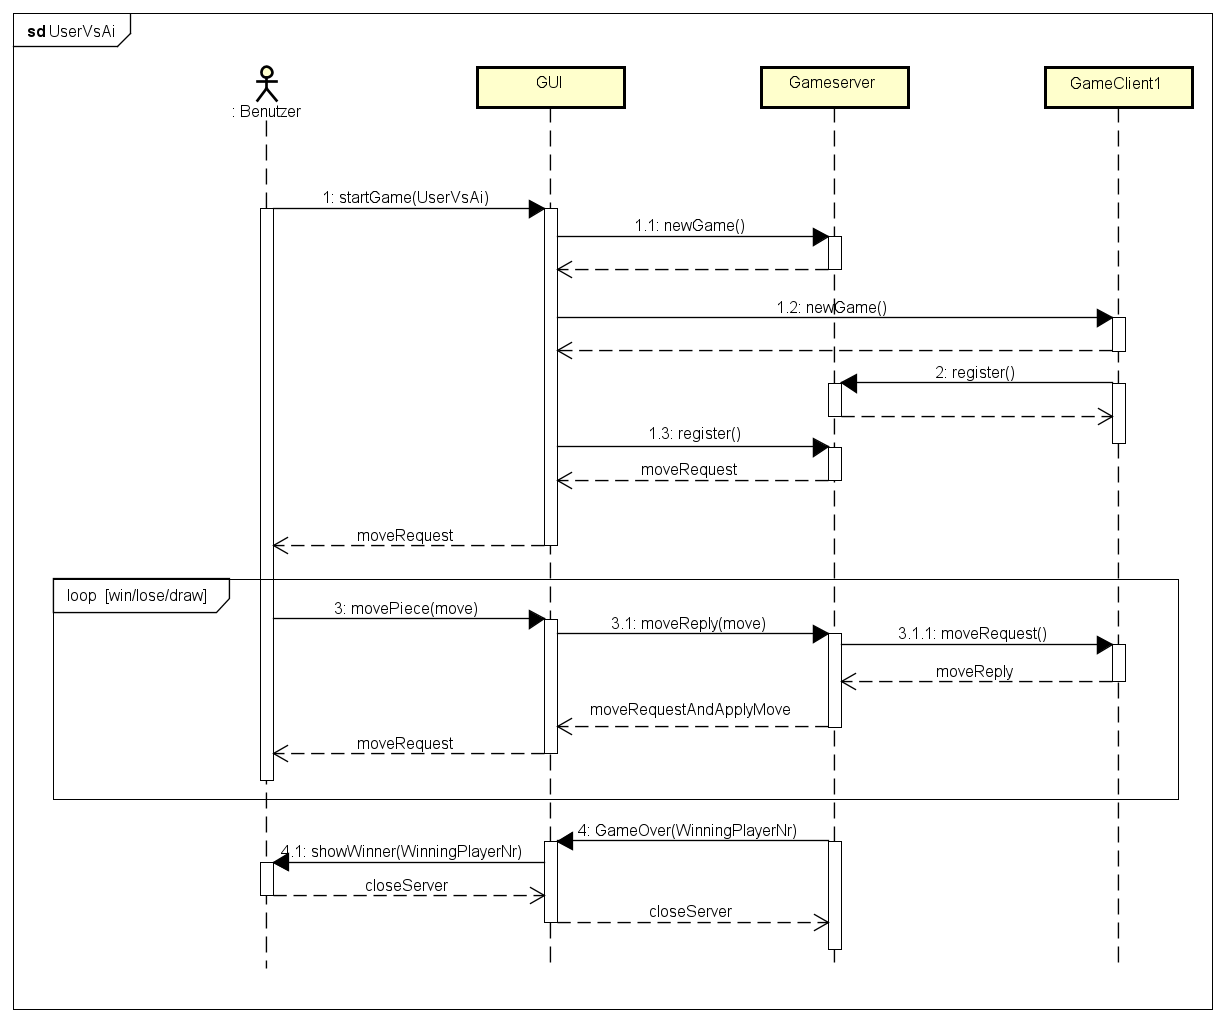
\includegraphics[width=0.83\linewidth]{pics/UserVsAiCommunication.png}
	\captionof{figure}{ Das \ac{UML} Sequenzdiagramm der Kommunikation von \ac{KI} gegen Benutzer}
	\label{fig:UserVsUserSequenceDiagram}
\end{minipage}
\\

Die Sequenzdiagramme für die Fälle \ac{KI} gegen \ac{KI} und Benutzer gegen Benutzer sind im Anhang im Kapitel \ref{apx:KommunikationDerKomp} 
der Seite \pageref{apx:KommunikationDerKomp} zu finden.

\pagebreak

\section{Hardware}
Dieses Kapitel setzt sich auseinander mit der verwendeten Hardware, für welche die Software erstellt worden ist. 
Die Ursprüngliche Idee des Projektes ist, ein Vorzeigeobjekt für Messen, wie den Tag der Informatik, zu haben.
Um dies zu realisieren, besteht die Hardware aus einem Touchscreen, welcher in einem tischförmigen Standfuß verankert 
und mit einem Raspberry Pi verbunden ist.

\subsection{Raspberry Pi}
Die Software wird auf einen Raspberry Pi Model 4 ausgeführt. Bei dem Betriebssystem handelt es sich um 
Raspbian, ein auf Debian basiertes Linux Betriebssystem. \cite{RaspberryPi} Da die Software auch mit anderen Betriebssystemen
kompatibel ist, könnte man den Pi durch ein beliebiges Gerät ersetzen, das eine Node.js Laufzeitumgebung unterstüzt.
Der Raspberry Pi ist jedoch aufgrund seiner Kosten und der Größe perfekt für das Projekt geeignet.
Die Installation der Software auf den Raspberry Pi ist in Kapitel \ref{apx:Installation} ``Erste Installation'' auf Seite \pageref{apx:Installation} des Anhangs beschrieben.
Zum Starten kann das Kapiel \ref{apx:appStarten} ``Starten der Anwendung'' auf Seite \pageref{apx:appStarten} des Anhangs verwendet werden.

\subsection{Touch Monitor}
Die Bedienung der Benutzeroberfläche erfolgt hauptsächlich über den Touchscreen, die Software kann jedoch auch auf normalen Monitoren ausgeführt werden.
Beim Touchscreen handelt es sich um den 27'' Llyama Touchscreen, welcher in einen Standfuß integriert ist. 
Eingaben können entweder durch Berührung des Touchscreens mit dem Finger oder mit einer klassischen Computermaus ausgeführt werden.
Für Texteingabe kann entweder das integrierte Softwarekeyboard, oder eine normale Tastatur verwendet werden.

\pagebreak

\section{Implementierung}
Diese Kapitel befasst sich mit den Implementierungsdetails auf, welche im Architektur noch nicht eingegangen wurden. 
Die verwendeten Programmiersprachen und Frameworks werden differenziert dargestellt, ebenso deren Auswirkungen deren auf 
die Implementierung.

\subsection{Programmiersprachen und Frameworks}
Da die Software aus mehreren individuellen Applikationen besteht, werden auch verschiedene Programmiersprachen und Frameworks für diese verwendet.
Im Folgenden werden alle Programmiersprachen und Frameworks, die Verwendung finden, erklärt.

\subsubsection{React.js}
Um die Software so kompatibel wie möglich zu gestalten, basiert der Frontend-Teil der Webapp auf Webtechnologie. Das bedeutet, dass jedes Endgerät, welches einen neueren 
Internetbrowser unterstützt, die Software zu einem Teil ausführen kann. Da eine Webseite in reinem Javascript, HTML und CSS zu schreiben viel Aufwand benötigt, 
wird ein Framework wie React.js verwendet. Bei React handelt es sich um eine Javascript Library zum Erstellen von Benutzeroberflächen.
Die Vorteile von React gegenüber Javascript stellen sich wie folgt dar:
\begin{itemize}
    \item Einfach, dynamische Websiten zu entwickeln
    \item Wiederverwertbare Komponenten
    \item Methoden und Markup gehören zusammen
    \item Funktionale Programmierung mit pure functions
\end{itemize}
Vor allem das erleichterte Erstellen von dynamischen Webseiten ist positiv zu bewerten, da die Benutzeroberfläche, während ein Spiel gespielt wird, dynamisch gehalten werden muss.
Im klassischen Javascript muss das Document Object Model (DOM) aufwendig verändert werden. Diese DOM-Manipulationen sind äußerst fehleranfällig und können Memoryleaks
verursachen. React sitzt hingegen zwischen Komponenten und dem DOM und übernimmt die komplette DOM-Manipulation.
Das Verwenden von Komponenten ist auch vorteilhaft, da zum Beispiel einzelne Spielfiguren als Komponenten festgelegt werden können 
und so mehrfach Code eingespart werden kann. 
Dabei ist das Besondere an React-Komponenten, dass sie einen ``Render'' Anteil besitzen, welcher eine JSX-Struktur zurückgibt. 
JSX ähnelt vom Code her HTML, kann aber dabei in Javascript verwendet und somit auch viel leichter direkt verändert werden \cite{React.js}.

\vspace{1em}
\begin{minipage}{\linewidth}
\lstinputlisting[caption=Ein Beispiel einer JSX Struktur aus dem Auswahlmenü Dame der Anwendung, label=lst:JSX,basicstyle=\ttfamily\scriptsize]{code/JSX.txt}
\end{minipage}

In Listing \ref{lst:JSX} zeigt eine JSX Struktur, in welcher man klassische HTML-Elemente wie \texttt{<h1>} oder \texttt{<div>}, aber auch Javascript wie 
\texttt{possibleMaps.length > 0}, erkennen kann.



\subsubsection{Node.js}
Der Gameserver, der Gameclient und das Backend der Webapp sind mit Node.js implementiert. 
Node.js ist eine asynchrone ereignisgesteuerte Javascript-Laufzeitumgebung, welche den Javascript-Code außerhalb des Webbrowsers ausführen kann.
Node.js wird hauptsächlich zur Programmierung von Netzwerkanwendungen, wie Webservern verwendet. Da der Großteil der Anwendung die
Kommunikation der einzelnen Komponenten ausmacht, ist speziell Node.js für dieses Szenario geeignet. 
Ein weiterer Vorteil von Node.js ist, dass es unabhängig vom Betriebssystem ist. Das bedeutet, dass die V8 Javascript-Laufzeitumgebung
auf dem Betriebssystem ausgeführt und dadurch die Node-Applikation dort zum Laufen gebracht werden kann.
\cite{Node}

\subsubsection{Typescript}
Node.js wird eigentlich in reinem Javascript geschrieben. Javascript leidet jedoch darunter, dass es keine Typisierung hat und sich somit leicht Fehler 
einschleichen können. Typescript ist eine auf Javascript basierende Programmiersprache, welche eine statische Typisierung unterstützt. 
Ähnlich wie bei C und C++ ist valider Javascript-Code auch valider Typescript-Code wodurch Typescript eine Obermenge von Javascript ist.
Nachdem Typescript-Code geschrieben wird, kann er in reines Javascript kompiliert werden.
Der Gameserver und der Gameclient sind in Typescript geschrieben, um Fehler durch die Typsicherheit zu verhindern. 

\subsubsection{C/C++ Node Add-ons}
Da Javascript eine im Vergleich sehr langsame Programmiersprache ist, wäre es sinnvoll, den künstliche Intelligenz Teil der Applikation, welcher für die 
Berechnung der nächsten Züge verantwortlich ist, in einer performanteren Sprache, die auch Memorymanagement bietet, wie C oder C++, zu schreiben. 
Node.js hat hierfür die Möglichkeit
Module mittels C++ zu implementieren und von deren Geschwindigkeit zu profitieren \cite{NodeC++Performance}. Ein C++ Node Add-on wird zu Maschinencode kompiliert, der von der
normalen Node-Anwendung über eine Javascript-Funktion ausgeführt werden kann. Der Vorteil zum reinen C++ ist, dass der Code in der V8 
Laufzeitumgebung ausgeführt wird, was ihn plattformunabhängig macht. \cite{C++Node}
Ein weiterer großer Vorteil ist die Verfügbarkeit von performanten C++ Libraries, welche speziell für Machine Learning geschrieben sind. 
In dieser Arbeit wird zwar kein Machine Learning verwendet, aber da für die \ac{KI}-Logik C++ benutzt wird, könnte man, bei einer Erweiterung 
um andere \ac{KI}-Algorithmen, Libraries wie Tensorflow benutzen.
%todo grafik die Laufzeitverbesserung zeigt

\subsection{Kommunikation}
Die Netzwerkkommunikation wurde bereits in Kapitel \ref{chap:Networkcom} auf Seite \pageref{chap:Networkcom} dargestellt und erklärt.
Im Folgenden wird die genauere Implementierung beschrieben.

\subsubsection{Verwendete Kommunkationstechnologie}
Da der Gameserver, der Gameclient und die Webapp eigenständige Prozesse sind, die nach Bedarf gestartet und gestoppt werden, benötigen sie eine 
Möglichkeit Nachrichten auszutauschen. Um dies zu gewährleisten, werden die von Node.js bereitgestellten \ac{TCP}-Sockets verwendet. 
Da \ac{TCP} ein Standardprotokoll mit Industriestandard ist, muss eine Komponente wie der Gameserver nicht unbedingt in der gleichen Programmiersprache 
wie der Gameclient implementiert sein, solange beide das selbe Protokoll mit der gleichen Codierung benutzen.
Falls man eine spezielle Python \ac{KI}-Library verwenden möchte, könnte man den kompletten Gameclient in Python schreiben.
\\
Der Vorteil von \ac{TCP}-Sockets, zum Beispiel im Vergleich zu \ac{UDP}, ist das Aufrechterhalten einer Verbindung. So muss sich der Client oder die \ac{GUI} nur einmal mit dem Server verbinden 
und kann im Laufe eines gesamten Spieles diese Verbindung nutzen. Ist ein Spiel zu Ende, kann die \ac{TCP}-Verbindung gekappt und die 
Sockets geschlossen werden. 
\\
Da es sich bei der Webapp um Webtechnologie handelt, welche in zwei Softwarepakete aufgeteilt ist, siehe Abbildung \ref{fig:ReversiXTGUIClassDiagram}, dem Frontend und dem Backend, verwenden 
diese Pakete auch eine eigene Netzwerkverbindung. Hierfür wird die Javascript Library Socket.io verwendet, die auf Websockets basiert.
Websockets funktionieren im Prinzip wie \ac{TCP}-Sockets, mit dem Unterschied, dass sie konstruiert wurden, um auf demselben Port wie HTTP zu laufen und vom 
Webbrowser unterstützt werden. Den entscheidenden Vorteil, den diese Technologie hat, ist neben der einfacheren Programmierung auch, dass Proxys, 
wie der in der Anwendung verwendete Reverse Proxy, sehr einfach mit Websockets umgehen können. So kann sich das Frontend, sobald es auf einem 
Mobilgerät aufgerufen wird, mit dem Backend auf dem Raspberry, über den Reverse Proxy verbinden, ohne dabei auf derselben Hardware zu laufen.

\subsubsection{Kommunikationsprotokoll des Gameservers}
Im Abschnitt \ref{chap:Networkcom} wird eine Kommunikation zwischen dem Gameserver und seinen Clients beschrieben, bei welcher der 
Server nur Anfragen eines festgelegten Protokolles akzeptiert. Das Protokoll für den Server orientiert sich stark am Protokoll
des Reversi-Gameservers und ist nur in einigen Stellen erweitert worden.

\begin{table}[H]
    \centering
    \begin{tabular} {|c|c|c|}
        \hline
        Typ (8-Bit-Integer) & Länge der Nachricht n (32-Bit-Integer) & Nachricht (n Bytes) \\
        \hline
    \end{tabular}
	\caption{Der Aufbau einer Nachricht}
    \label{tab:Nachritenaufbau}
\end{table}

In Tabelle \ref{tab:Nachritenaufbau} ist der Aufbau einer Nachricht dargestellt. Es gibt ingesamt neun verschiedene Nachrichtentypen. Dazu gehören unter anderem
``neues Spiel starten'', ``Zugaufforderung'' und ``Spiel Ende''. Weitere Details findet man in Kapitel \ref{apx:Protokoll} auf Seite \pageref{apx:Protokoll} des Anhangs. 
Die meisten Nachrichten eines gewissen Typs haben immer die gleiche Länge. Es gibt jedoch
Ausnahmen, wie die Nachricht zum Senden des Spielfelds, bei welcher ein 10x10 oder 8x8 Damespielbrett gewählt werden kann. Der eigentliche Inhalt der Nachricht entspricht dann 
den Daten, die übertragen werden, wie zum Beispiel den Feldern, welche bei einem Spielfeld besetzt sind, oder das Ursprungsfeld und das Zielfeld bei einer Zugantwort. 
Das Einhalten dieses Protokolls ist sehr wichtig, denn nur so kann garantiert werden, dass zwei Komponenten auch wirklich miteinander kommunizieren können.

\subsubsection{Dynamische Portsuche}
Da es möglich sein muss, dass mehrere Gameserver gleichzeigt laufen können, muss beachtet werden, dass sich diese nicht mit den selben \ac{TCP}-Port aussuchen können.
Deswegen bekommt das Backend der Webapp ein Interval, aus welchem es die Ports des Gameservers wählen darf. Es versucht somit einen freien Port zu finden, der noch nicht 
besetzt ist. Das Szenario, das mehrere Gameserver laufen, ist nicht sehr unwahrscheinlich. Sollten sich mehrere Benutzer mit ihren Smartphones mit der Anwendung verbinden,
so muss für jeden, der ein Spiel beginnt, ein eigener Gameserver starten. Einen weiteren Vorteil, den diese Dynamik bietet, ist, dass die Simulationen 
zum Testen der Software parallel zur normalen Anwendung laufen können. Bei der verwendeten Library, die für diese Fälle gedacht ist, handelt es sich um 
das Node.js NPM-Paket ``node-portfinder'' \cite{portfinder}. In der Anwendung wird die Portfinder-Library in jeder Komponente verwendet. Sollte 
eine Komponente unabhängig von den anderen gestartet werden und ihr Port bereits belegt sein, sucht sie sich einen eigenen.

\subsection{Erweiterungen der graphischen Benutzeroberfläche}
Im Grundlagenkapitel findet man eine Erklärung zur vorhandenen \ac{GUI}, siehe Kapitel \ref{chap:gegebeneApp} auf Seite \pageref{chap:gegebeneApp}, welche 
um weitere Menüs erweitert worden ist. Da die Anwendung vor der Erweiterung um das Spiel Dame nur Reversi als Spiel hatte, 
braucht sie ein weiteres Menü um zwischen den verschiedenen Spielen wählen zu können.

\vspace{1em}
\begin{minipage}{\linewidth}
	\centering
	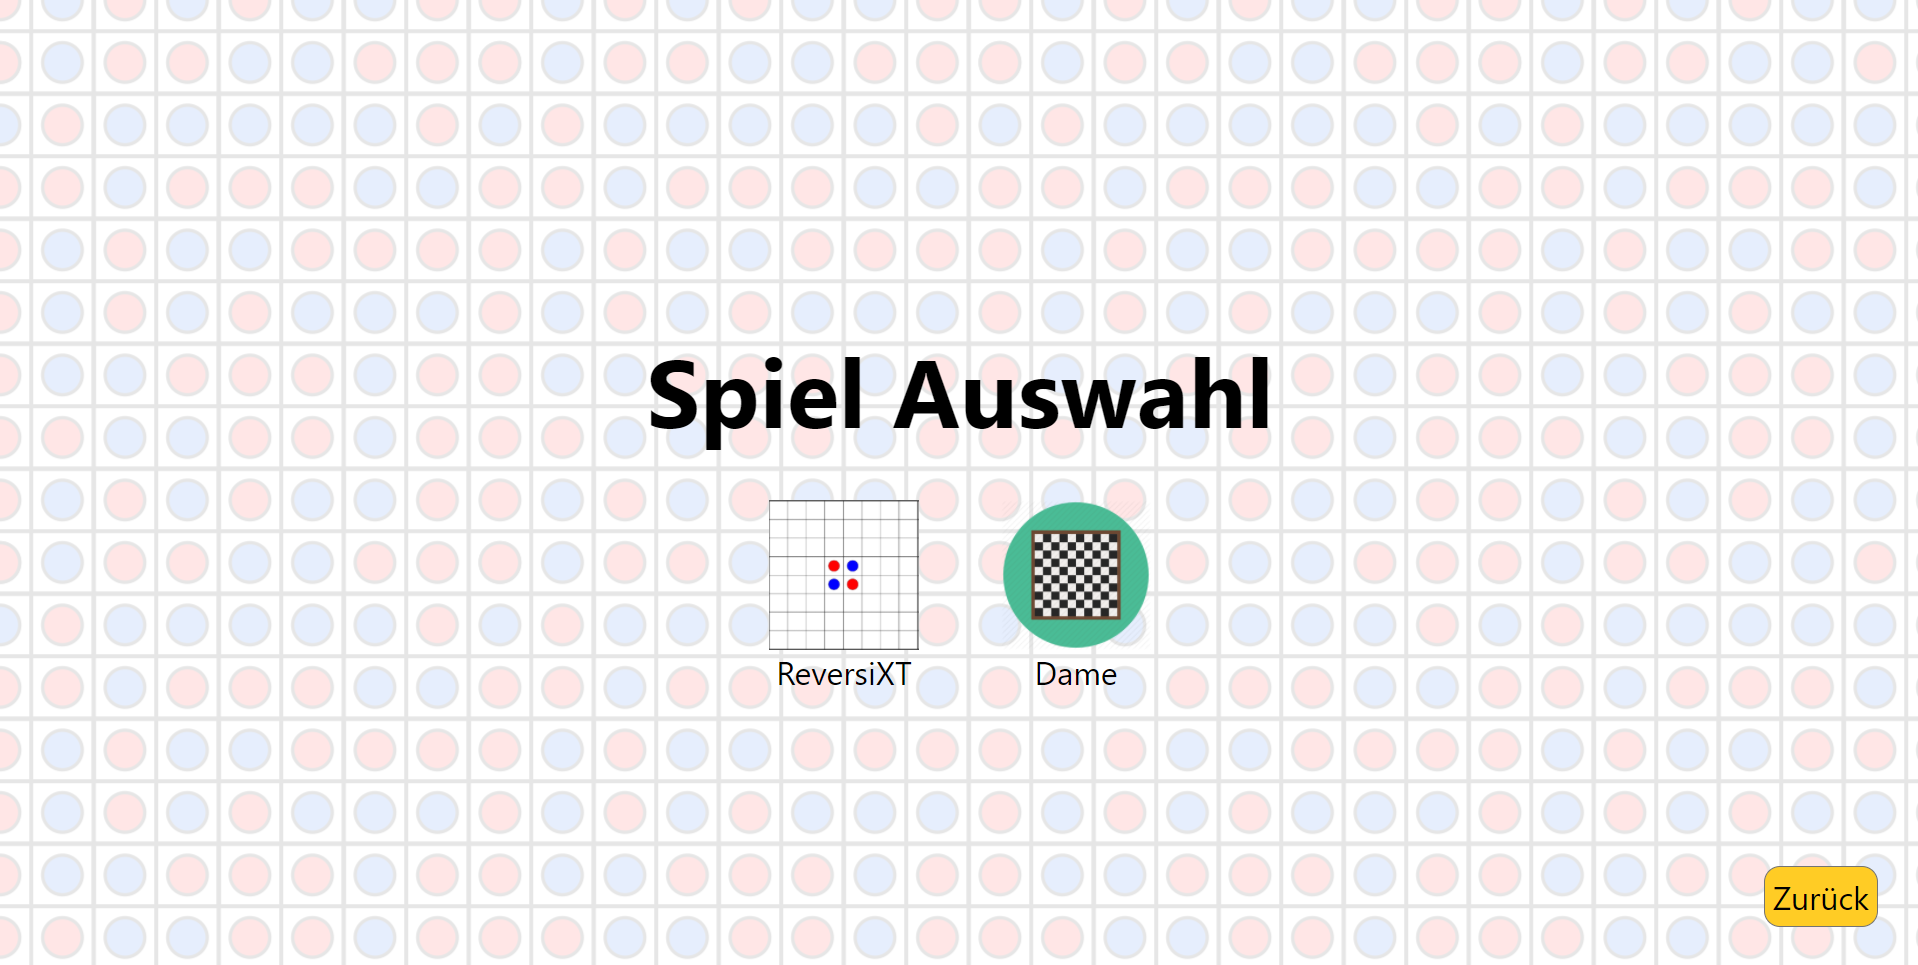
\includegraphics[width=0.7\linewidth]{pics/GameSelectionScreen.png}
	\captionof{figure}{ Das Auswahlmenü für die verschiedenen Spiele }
	\label{fig:GameSelectionScreen}
\end{minipage}
\\

Die Abbildung \ref{fig:GameSelectionScreen} zeigt zwei Buttons, mit Links auf die \ac{URL} Pfade der Spieleinstellungen der jeweiligen Spiele. 
Das nächste Menü, das dadurch erreicht wird,
entspricht entweder dem schon vorhandenen Auswahlmenü von Reversi oder dem neuen für Dame, welches in Abbildung \ref{fig:Auswahlmenue} zu sehen ist.

\vspace{1em}
\begin{minipage}{\linewidth}
	\centering
	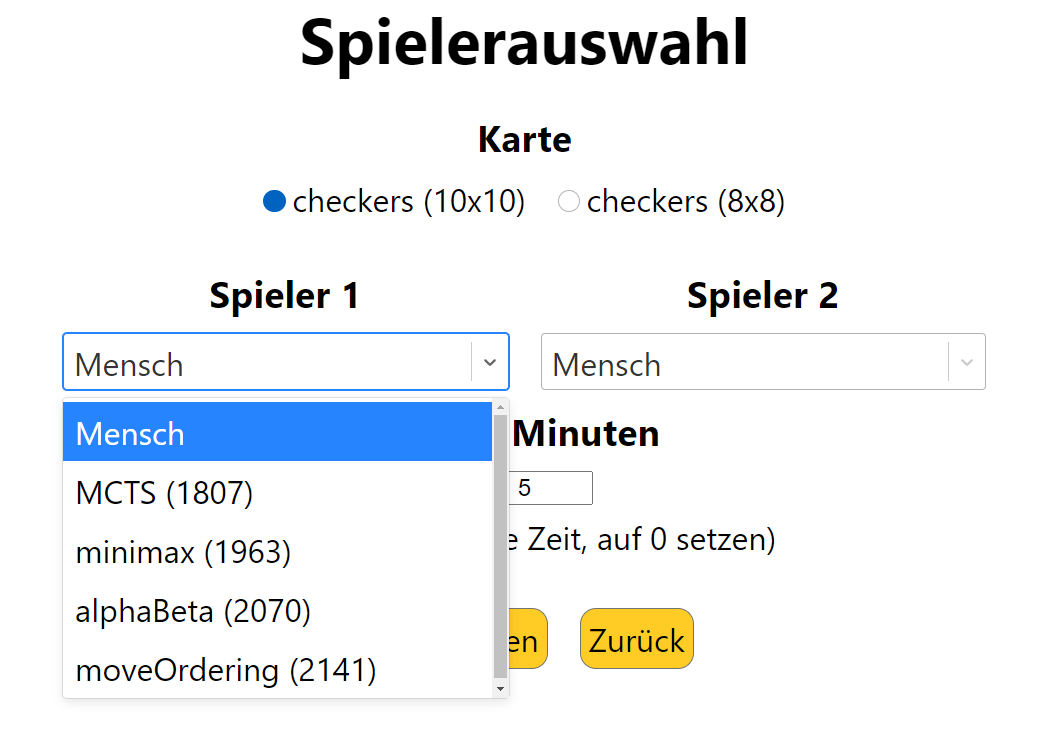
\includegraphics[width=0.7\linewidth]{pics/AlgorithmeninderApplikation.png}
	\captionof{figure}{ Das Auswahlmenü für ein Damespiel }
	\label{fig:Auswahlmenue}
\end{minipage}
\\

Direkt nachdem dieses Menü aufgerufen wird, schickt das Frontend eine Nachricht über Websockets an das Backend, um alle Karten, die im Ordner ``maps'' liegen, sowie 
alle Algorithmen, die in algorithms-consts.js des Gameclients vermerkt sind, zu bekommen. Außerdem wird die elo.txt Datei, die durch 
Simulation erzeugte Elo-Werte für die Spielstärke aufweist, benutzt, um die jeweilige Stärke der Algorithmen zu zeigen, was in der Abbildung 
dem Wert in Klammern entspricht. Unter der Spielerauswahl befindet sich eine Eingabe für die Zeit in Minuten, welche die maximale Zeit,
die ein Spieler für ein Spiel zur Verfügung hat, angibt. Wird diese auf 0 gesetzt, taucht ein weiteres Menü auf, das aber dieses Mal eine 
Suchtiefe fordert. Durch das Klicken auf ``Starten'' gelangt man zu der Seite, die das eigentliche Spiel darstellt, siehe Abbildung \ref{fig:DameSpielSeite}.
Bei den Buttons, Radiobuttons und der Dropdown-Liste handelt es sich um HTML-Elemente, die mittels CSS gestylt sind und durch 
des Javascript von React.js Aktionen ausführen.

\vspace{1em}
\begin{minipage}{\linewidth}
	\centering
	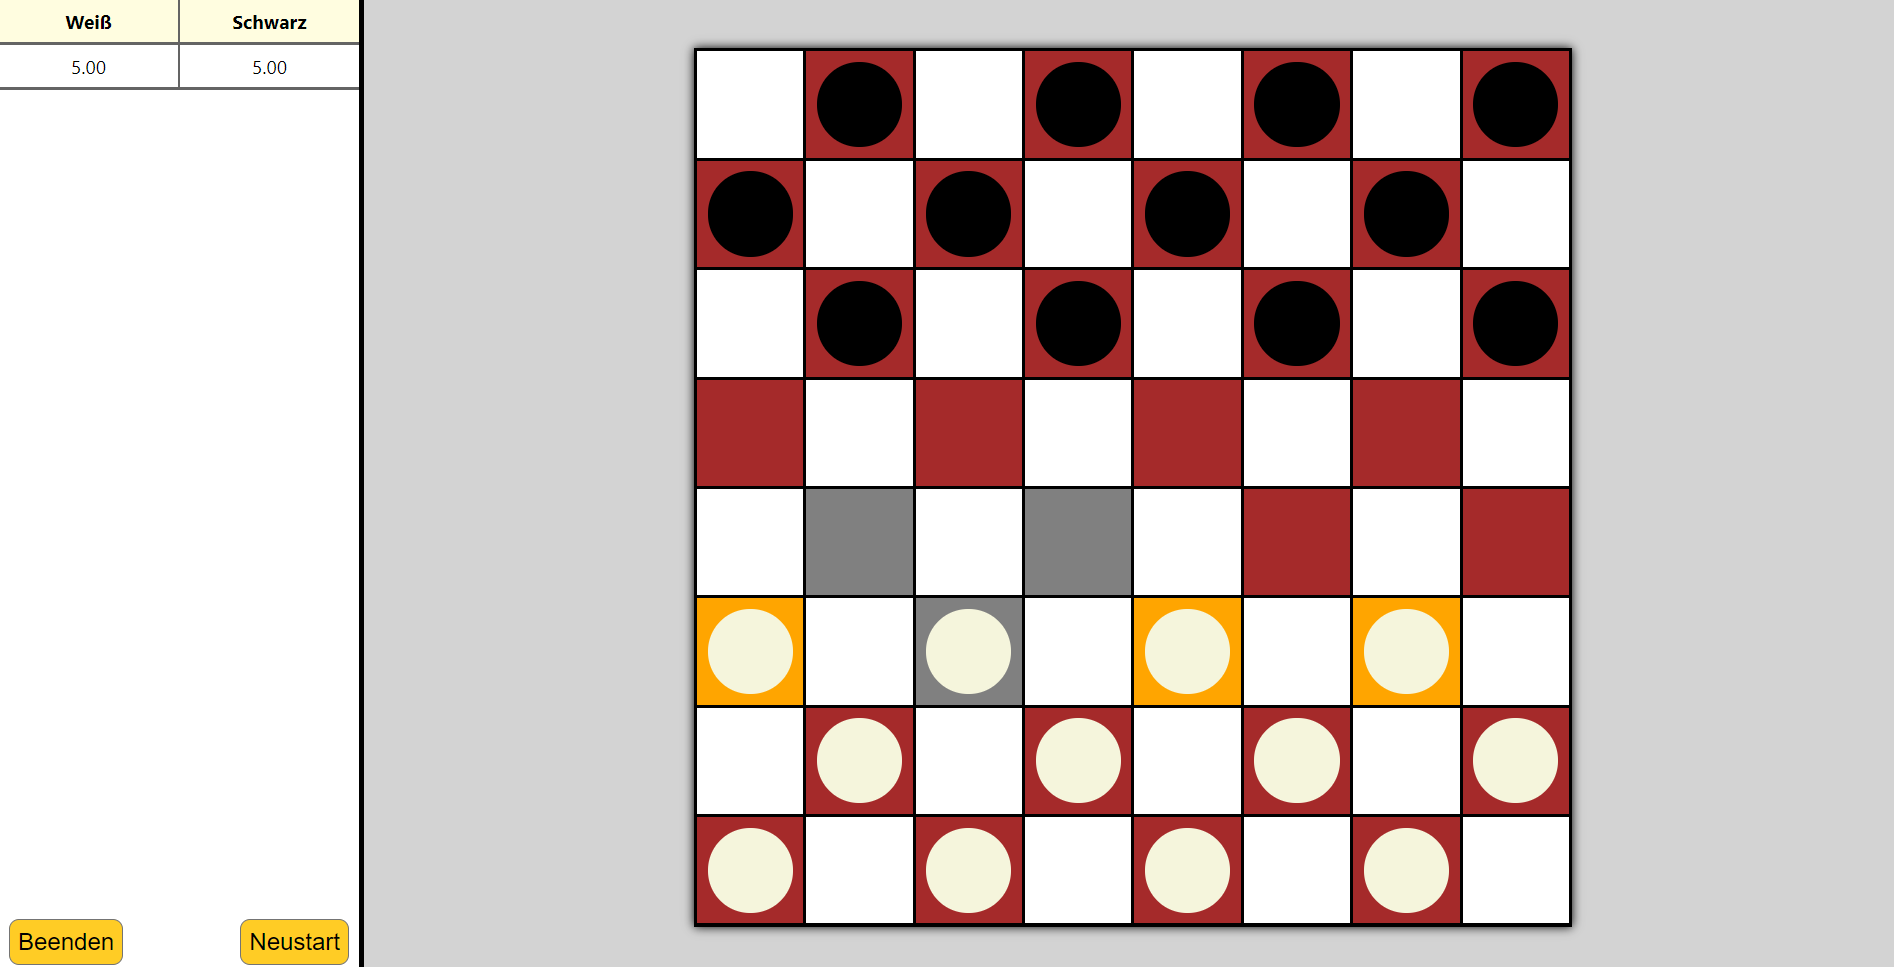
\includegraphics[width=0.7\linewidth]{pics/DameWebsiteSpiel.png}
	\captionof{figure}{ Die Seite zur Darstellung des Spielfeldes }
	\label{fig:DameSpielSeite}
\end{minipage}
\\

Diese Seite zeigt das Damespielfeld mit der Informations-Sidebar, welche die Restzeit pro Spieler anzeigt.
Auf dem Spielfeld sind die Damespielsteine durch die Farben Schwarz und Weiß, als Scheiben dargestellt. 
Ist das Spielfeld hinter dem Stein gelb markiert, bedeutet das, dass er gezogen werden darf. 
Durch das Klicken eines solchen gelb hinterlegten Steines werden alle Felder, auf welche der Stein ziehen darf,
grau markiert dargestellt. Um dieses ``Markieren'' und ``nächsten Zug finden'' zu ermöglichen, verwendet das Frontend Funktionen,
welche den Funktionen der Spiellogik-Dame ähneln.
\\
Bei den Spielsteinen und dem Spielfeld handelt es sich um React.js Komponenten, die mittels JSX und CSS ihre Form bekommen.
Jeder Spielstein hat eine Callback Methode, die nach einem Klick aufgerufen wird. Je nach Position und 
Ergebnis der \texttt{CheckersAllPossibleMoves} Funktion, werden die richtigen Felder auf dem Spielfeld markiert.

\subsection{Mobile Anbindung}
Für die Anbindung der Mobilgeräte an die Software muss die Software nicht elementar umgestaltet werden. 
Da es sich bei der Software um eine React.js Anwendung handelt und sie auch auf dem Touchscreen im Webbrowser als Website 
ausgeführt wird, kann sie problemlos mit nur kleinen Anpassungen auf dem Browser eines Smartphones laufen.
CSS Stylesheets bieten eine Möglichkeit das Gerät, welches auf die Website zugreift, zu erkennen und 
dadurch das Layout und Design anzupassen. So muss keine Logik verändert werden, sondern nur die Art wie die Website dargestellt wird.
\\
Die eigentliche Verbindung wird über die lokale IP-Adresse des Netzwerks, in der sich 
die Hardware befindet, getätigt. Um die Adresse für das Smartphone zu bekommen, ist in der graphischen Oberfläche im 
Hauptmenü ein QR-Code eingebaut. Der QR-Code wird zum Start der Anwendung neu mit Hilfe einer Javascript Library generiert,
dadurch ist die Software unabhängig vom Netzwerk in dem sie sich befindet. Scannt ein Gerät diesen Code, bekommt es einen Link auf das Auswahlmenü von Dame. Würde ein weiteres
Spiel zur Software hinzufügen werden, könnte die Software um einen weiteren QR-Code erweitert werden. 
Abbildung \ref{fig:QRCodeScreen} zeigt das Hauptmenü, mit dem QR-Code, der unten zentral plaziert wurde.

\vspace{1em}
\begin{minipage}{\linewidth}
	\centering
	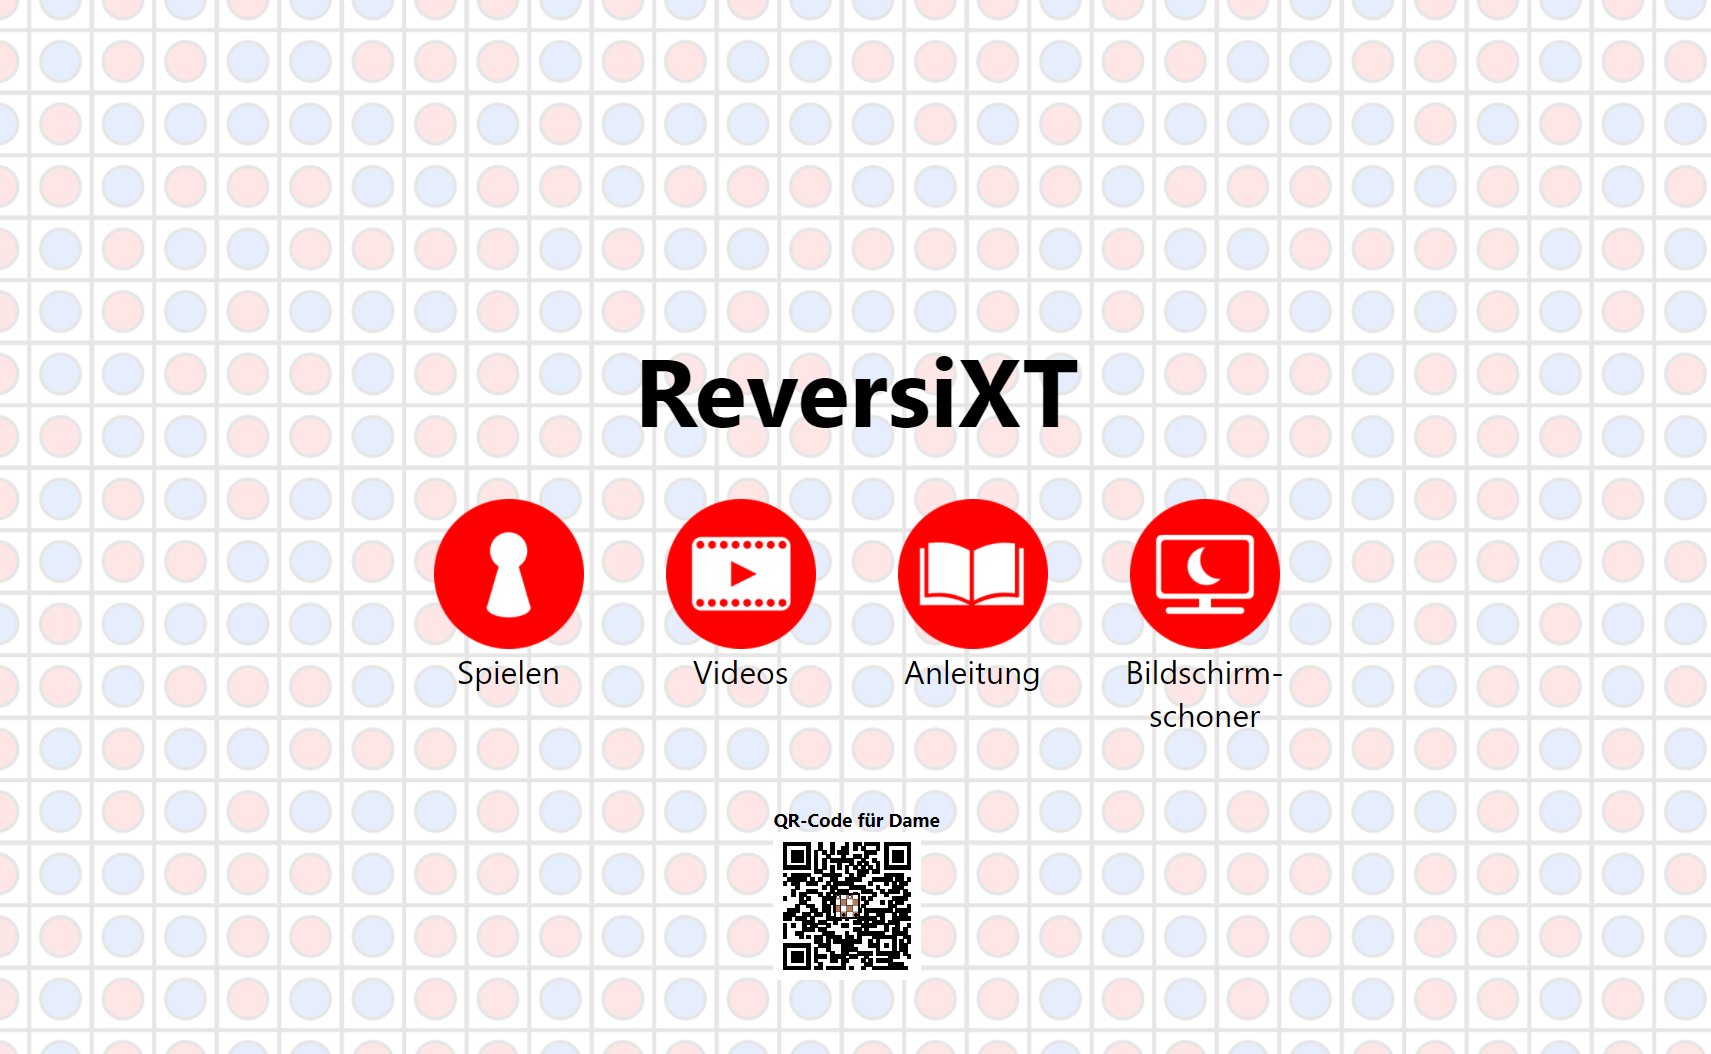
\includegraphics[width=0.7\linewidth]{pics/mainMenuWithQR.png}
	\captionof{figure}{ Das Hauptmenü mit dem QR Code }
	\label{fig:QRCodeScreen}
\end{minipage}
\\

Damit kein Zugriff auf andere Ports oder Funktionen des Raspberry Pis möglich ist,
wird ein Reverse Proxy verwendet, welcher jeden Zugriff überprüft und nur gültige durchlässt. Beim verwendeten Reverse Proxy handelt 
es sich um die Software Nginx. Nginx ist eine Webserver-Software, welche als Load Balancer, Mail Proxy, HTTP cache und auch 
als Reverse Proxy verwendet werden kann. Weitere Informationen zur Konfiguration und Installation können in Anhang Kapitel \ref{apx:Installation} 
auf Seite \pageref{apx:Installation} gefunden werden.


\subsection{Gameclient C++ und Typescript Kompatibilitätsschicht}
Die Besonderheit der Implementierung des Gameclients basiert darauf, dass es sich um eine Applikation handelt, welche in zwei verschiedenen 
Programmiersprachen geschrieben ist. Zum einen wird die durch Node.js verwendete Sprache Typescript für den Netzwerk und Validierungs Teil 
verwendet und zum anderen C++ für die Performance der \ac{KI}-Algorithmen. Man hätte auch die Anwendung komplett in C++ schreiben können,  
dann wäre es aber nicht möglich, gewesen die schon geschriebene Netzwerkkomponente des Gameservers wiederverwenden. Auch die Kompatibilität würde etwas darunter leiden, da 
bei C++ beachtet werden muss, dass Libraries für verschiedene Betriebssysteme verfügbar sein müssen und diese eventuell mit anderen 
Compilern bearbeitet werden. 
\\
Um einen reibungslosen Übergang zwischen den beiden Programmiersprachen zu garantieren, wird eine Klasse als reine Kompatibilitätsschicht verwendet.
Alle Funktionen und Umwandlungen, die für das Konvertieren nötig sind, werden in dieser Klasse zusammengefasst. Dies erlaubt, dass der restliche 
C++ Code auch unabhängig kompiliert werden kann, ohne Node.js Add-on spezifische Details zu benötigen, was ein leichteres Testen erlaubt.
In Abbildung \ref{fig:KIClientClassDiagram} auf Seite \pageref{fig:KIClientClassDiagram} wird diese Umwandlung in der Klasse \texttt{CheckersAi} 
vorgenommen.

\subsection{Verwendete \ac{KI}-Algorithmen}
\label{chap:KIAlgorithms}
In Kapitel \ref{chap:Grundlagen} wurden einige \ac{KI}-Algorithmen beschrieben, welche auch im Damespiel der Applikation implementiert sind.
Die Applikation bietet vier Algorithmen zur Auswahl an, gegen die der Spieler antreten kann, siehe Abbildung \ref{fig:Auswahlmenue} auf Seite \pageref{fig:Auswahlmenue}. 
Diese Algorithmen sind, Minimax, Alpha-Beta-Pruning, Zugsortierung und \ac{MCTS}.
Der Abbildung \ref{fig:KIClientClassDiagram} auf Seite \pageref{fig:KIClientClassDiagram}
kann man entnehmen, dass es zwei Hauptalgorithmen in dem Paket CheckersAiLogik gibt. Minimax und \ac{MCTS}. Diese Aufteilung kann vorgenommen werden,
da Alpha-Beta-Pruning und Zugsortierung auf Minimax basieren.


\subsubsection{Minimax}
Der Minimax-Algorithmus wird, wie in \ref{chap:Minimax} auf Seite \pageref{chap:Minimax} erklärt, durch einen Baum repräsentiert. Dadurch, dass jeder Knoten einen Spielbrettzustand
repräsentiert und durch den Algorithmus einen Wert zugewiesen bekommt, hat die Applikation eine \texttt{MinimaxNode}-Klasse.
Diese Klasse ist hauptsächlich für das Speichern der Informationen zuständig, welche dann einfach von der eigentlichen \texttt{Minimax}-Klasse zur Berechnung
verwendet werden können. Damit ein vollständiger Baum aufgebaut werden kann, enthält die \texttt{MinimaxNode}-Klasse ein Array mit Zeigern auf allen 
Kindknoten, was eine Vorwärtstraversierung des Baumes erlaubt. 
Um eine Berechnung zu starten, braucht die \texttt{start}-Funktion ein Spielbrett, den Spieler, der an der Reihe ist, eine
Tiefe bis zu der berechnet werden soll und bzw. oder ein Zeitlimit. Ist ein Zeitlimit angegeben, so benutzt die \texttt{start}-Funktion Iterative Deepening, siehe Kapitel
\ref{chap:IterativeDeepening}, dadurch kann die Berechnung so gut wie möglich die komplette Zeit ausnutzen. Ist kein Zeitlimit angegeben, 
wird die spezifizierte Tiefe dem Minimax übergeben und dieser rechnet so lange, bis er diese erreicht. Wird Minimax mit Iterative Deepening gestartet,
wird ein Zeitwert zum Anfang gespeichert. Dieser Zeitwert wird während der Berechnung von Minimax mit dem momentanen Zeitwert verglichen. Ist die 
Differenz dann größer als des Zeitslimits oder entspricht diesem, wird mittels einer C++ Exception die momentane Berechnung abgebrochen und nach dem Zurückkehren in 
den Catch-Block der letzte komplett berechnete Zug verwendet. 
Wird Minimax gestartet, holt sich der Algorithmus unter Verwendung der Funktion AddAllChildren, alle Kinderspielbretter. Diese 
definieren sich aus allen möglichen Zügen, die von einer Stellung aus möglich sind, siehe Kapitel \ref{chap:Spiellogik}. Der Vorgang wird 
rekursiv wiederholt, bis die geforderte Tiefe erreicht und die Bewertungsfunktion aufgerufen wird. Die Ergebnisse werden dann rekursiv rückwärts in 
den MinimaxNodes des Baumes eingetragen.

Um mit Minimax den besten Zug berechnen zu können, wird eine gute Bewertungsfunktion 
benötigt. Die verwendete Funktion hat folgende Eigenschaften:
\begin{itemize}
    \item Normale Figur: +1 für Weiß und -1 für Schwarz
    \item Dame: +3 für Weiß und -3 für Schwarz
    \item Spielende: $\infty$ für Weiß und -$\infty$ für Schwarz
\end{itemize} 
Etwaige Erweiterungsmöglichkeiten wären, bedrohte Figuren, sowie Figuren in der Spielmitte und in den Grundreihen mit in die Berechnung einfließen zu lassen.
Dabei ist zu berücksichtigen, dass eine komplexere Bewertungsfunktion mehr Berechnungszeit benötigt, aber bessere Ergebnisse liefern könnte.

\subsubsection{Alpha-Beta-Pruning}
Da, dass Alpha-Beta-Pruning eine Erweiterung von Minimax ist, kann dieser Algorithmus mit in die Minimax-Klasse gepackt
und über Übergabeparameter des Konstruktors an- und ausgeschalten werden. Dadurch hat man weniger Code, kann aber trozdem noch 
verschiedene Algorithmen mit unterschiedlicher Stärke im Menü wählen. Da Minimax rekursiv implementiert ist, kann Alpha-Beta-Pruning sehr elegant mit wenigen 
Zeilen Code geschrieben werden. In Listing \ref{lst:AlphaBetaCode} sieht man die einfache Implementierung des Alpha-Beta-Prunings im Maximierer Teil 
von Minimax. Zuerst wird überprüft, ob es sich um reinen Minimax handelt, oder um Alpha-Beta beziehungsweise Zugsortierung. Danach wird der Alpha Wert mit dem
Maximum aus dem alten Alpha Wert und dem, durch die Bewertungsfunktion berechneten, eval Wert berechnet. Das Codestück im Minimierer hätte an dieser Stelle 
ein Min anstelle des Max. Das Pruning findet für den Fall, dass Beta kleiner gleich Alpha ist, statt. So wird der Teil dieses Zweiges nicht weiter untersucht.
\vspace{1em}
\lstinputlisting[caption=Code der Implementierung des Alpha-Beta-Prunings, label=lst:AlphaBetaCode,basicstyle=\ttfamily\scriptsize]{code/Alpha-Beta.txt}

\subsubsection{Zugsortierung}
Ähnlich wie Alpha-Beta-Pruning ist die Zugsortierung eine Erweiterung von Minimax und befindet sich deshalb auch in der selben Klasse und kann über den 
Konstruktor ausgewählt werden. 
Um eine Zugsortierung im Minimax zu erreichen, wird im Teil von AddAllChildren des Minimax die Bewertungsfunktion der Zugsortierung aufgerufen.
Dadurch, dass es sich um Array von Zeigern handelt, welche auf die Kindknoten zeigen, muss nur dieses Array unter Berücksichtigung der Bewertungsfunktion
sortiert werden, was durch die Hilfe der C++ Standardbibliothek sehr einfach zu implementieren ist. Es ist hier besonders wichtig, eine effiziente und einfache Funktion für die 
Bewertung zu haben. Sie sollten einfacher als die eigentliche Bewertungsfunktion von Minimax sein. Man sollte die Sortierung nicht komplett bis zur letzen Suchtiefe anwenden, 
da eine Sortierung am Anfang sehr viele Zweige ausschließen kann und später nicht mehr so effektiv ist. Da aber auch die Suchtiefe, durch das Verwenden der Zeit bei 
unterschiedlicher Hardware, immer unterschiedlich ist, muss der Wert für die Tiefe, bis zu welcher Zugsortierung angewandt wird immer neu angepasst werden.
Die momentane Implementierung speichert die zuletzt erreichte Suchtiefe und multipliziert diese mit 1/3, wodurch nur das erste Drittel des Baumes sortiert wird. 
Um die Performance weiter zu verbessern, kann hier eine bessere Heuristik verwendet werden.


\subsubsection{\ac{MCTS}}
Der \ac{MCTS}-Algorithmus ist ein auf Simulation basierender Algorithmus, der bereits in Kapitel \ref{chap:MCTS} erklärt wurde.
Ähnlich wie beim Minimax-Algorithmus verwendet der \ac{MCTS}-Algorithmus ebenso einen Baum mit Knoten, welche den Spielbrettzustand halten.
Der Unterschied liegt hier bei den Informationen, die ein Knoten hält. Eine \texttt{MCTSnode} hält die Anzahl an verlorenen und gewonnen Spielen,
die aus der Simulation hervorgehen. Jeder Knoten hat ein Array mit Zeigern auf seine Kinderknoten, wodurch die bekannte Baumstruktur entsteht.
Im Gegensatz zur \texttt{MinimaxNode} werden nicht pro Iteration alle Kinder eines Knotens mit \texttt{AddAllChildren} hinzugefügt, sondern mittels des 
\ac{UCT}-Ergebnisses wird der beste Kandidat gewählt. Für den Parameter $c$ wird Zwei gewählt, da in vielen gelungenen Spielen die Zahl Zwei 
zu guten Erfolgen geführt hat. Da der \ac{MCTS} nicht unendlich lange simulieren soll, braucht er ein Zeitlimit oder eine vorgegebene Anzahl an Simulationen,
nach welchen er die Simulation abbrechen und das Ergebnis zurückliefern soll. Die Zeitüberprüfung erfolgt ähnlich wie bei Minimax.
Ist der Zeitpunkt zum Abbruch gekommen, wird eine C++ Exception geworfen, was zum Stop der Simulation führt. 
Das Ergebnis des \ac{MCTS} ist der Kindknoten, welcher den besten Wert nach den Simulationen hat, dieser wird auch vom Algorithmus zurückgegeben.

\subsection{Dame Spiellogik Implementierung}
Die Spiellogik von Dame ist an mehreren Stellen der Software redundant zu finden und somit auch ausschlaggebend für die verwendete Programmiersprache.
Ein Hauptgrund den Gameclient nicht komplett in C++ zu schreiben ist, neben der Netzwerkkommunikation, auch die Wiederverwendung der Spiellogik.
Da die Implementierung in Typescript im Gameserver und Gameclient vorfindbar ist und keine anderen Libraries verwendet, kann es von diesen in Javascript kompiliert 
und auch im Frontend der React.js Anwendung verwendet werden.
\\
Eine Besonderheit bei der Implementierung des Gameclients ist, dass er zwei Implementierungen der Spiellogik hat, 
einmal in C++ für die \ac{KI}-Logik und ein zweites Mal in Typescript, für die Zugvalidierung eines neuen Zuges. 
Das dabei betroffene Paket ist das \texttt{Checkers}-Paket aus Abbildung \ref{fig:KIClientClassDiagram} von Seite \pageref{fig:KIClientClassDiagram}. 
\\
Die eigentliche Implementierung ist, bis auf einen Sonderfall für beide Sprachen, in der \texttt{move} Methode der \texttt{MoveApplier} Klasse identisch, 
welche im Verwendungszweck liegt. So wird eine Variante benötigt, die alle neuen Züge validiert und das Spielfeld durch diese anpasst. Die andere Variante ist für 
die Zugberechnung der \ac{KI} verantwortlich. Wird also ein Minimax Baum aufgebaut, welcher als Knoten einen Spielfeldzustand hat, muss diese Methode für jeden möglichen Zug eines 
Spielfeldes aufgerufen werden, um alle seine Kindknoten zu erstellen. Bei solchen Bäumen mit hoher Suchtiefe kann es schnell passieren, 
dass diese Methode sehr oft ausgeführt wird. Diese Implementierung braucht deswegen keine Validierung, da davon ausgegangen werden kann, dass die bisherigen Züge der 
Berechnung korrekt waren. Dadurch wird die Performance extrem verbessert, wodurch auch höhere Suchtiefen erreichbar sind.
Ein weiterer Grund für die Redundanz des \texttt{Checkers}-Paketes ist die Verwendung der beiden Sprachen C++ und Typescript in einer Anwendung. 
Es wäre zwar möglich, von C++ aus die vorhandene \texttt{MoveApplier}-Klasse in Typescript aufzurufen, jedoch wird durch den Kompatibilitäts-Layer Overhead erzeugt,
welcher zwar gering ist, sich aber bei vielen Aufrufen summiert. Außerdem ist eine Implementierung in C++ schneller als das von Typescript kompilierte Javascript.
\\
Die durch Typescript implementierte Variante ist dieselbe, wie die im Gameserver verwendete und dient rein zur Validierung aller eingehenden Züge. Im Gegensatz zum Gameserver 
bräuchte der Gameclient keine Validierung, da er davon ausgehen kann, dass der Gameserver nur korrekte Züge schickt und er eigentlich nur von diesem seine 
neuen Züge bekommt. Jedoch soll der Gameclient auch sicher vor böswilligen Benutzern sein, welche falsche Züge an den Gameclient schicken könnten und falls ein Fehler,
der die Nachricht verändert, in der Netzwerkverbindung auftreten sollte, wird diese trotzdem erst überprüft.
\\
Zum Prüfen aller Züge oder zur Zugsuche gibt es Methoden, welche entweder alle normalen Züge angeben oder alle Züge, bei denen ein Schlag erzwungen wird. 
Diese Züge werden mittels dieser Methoden gesucht und danach über die \texttt{Move}-Klasse abgebildet. Der Rechen- und Speicheraufwand ist hierbei vor allem 
für normale Figuren relativ gering. Damen können jedoch wesentlich mehr Züge generieren, was zu längeren Rechenzeiten, insbesondere bei \ac{KI}-Algorithmen führt.
\\
Die Implementierung der Suche aller normalen Züge ist relativ einfach. So werden bei normalen Spielfiguren die beiden Felder schräg links und rechts vor ihr 
auf ein leeres Feld geprüft und bei einer Dame alle Felder, bis ein nichtleeres Feld auftaucht. Etwas schwieriger gestaltet sich jedoch das Finden aller 
Züge von Damen, die einen Schlagzwang fordern. Normale Figuren sind auch hier recht leicht zu finden. Ist schräg rechts oder links vor der Figur 
eine gegnerische, muss nur das Feld dahinter auf ein leeres Feld geprüft werden. Bei Damen hingegen, muss in alle Richtungen bis zum Spielfeldrand 
geprüft werden, ob sich in ihrem Weg ein Gegner befindet und ob ein Feld oder mehrere Felder hinter dem Spielstein vorhanden sind. Dadurch kann es sein, dass ein 
Damespielstein sehr viel Zugmöglichkeiten zum Schlagen hat, was vor allem für eine höhere Rechenzeit bei \ac{KI}-Algorithmen sorgt, sobald eine Dame dem Spielfeld hinzugefügt wird.


\subsection{Berechnung des Zeitlimits}
In Kapitel \ref{chap:timelimit} ist bereits erklärt, wie die Zeitberechnung aufgebaut ist. Dieser Abschnitt zeigt die Implementierungsdetails.
Dadurch, dass nach jedem Zug ein Zeitlimit geschickt wird, wie lange ein \ac{KI}-Algorithmus Zeit zu rechnen hat, muss dieses Limit ein Bruchteil 
der gesamten Zeit sein, welches für den momentanen Zug benutzt werden soll. Um die durchschnittliche Dauer eines Damespieles bestimmen zu können,
braucht man einen Datensatz, der die Zuganzahl mit angibt. Die ``American Checkers Federation'' (AFT) bietet eine Datenbank von 9374 Spielen,
aus der man die Durchschnittsanzahl an Zügen pro Spiel ausrechnen kann \cite{CheckersFederation}. Ein durchschnittliches Spiel 
dauert ungefähr 49 Züge. Um so ein Zeitlimit berechnen zu können, bekommt jeder Gameclient vom Gameserver eine Zugzahl von 30 Zügen, die nach jedem Zug 
dekrementiert wird. Die 30 Züge kommen aus dem Grund zustande, dass die 24 um 6 erhöht werden, um etwas Toleranz zu haben, denn erreicht man 
eine sehr niedrige Zahl, würde ein Algorithmus nur wenige Sekunden zum Rechnen bekommen. Deswegen wird ab einem Wert von 5 Zügen, 
dieser nicht weiter dekrementiert. Der Wert an Zügen wird durch 
die restliche Zeit geteilt, wodurch man eine ungefähre Zeit für diesen Zug bekommt. Diesem Wert kann man noch etwas variieren, um 
ein besseres Ergebnis zu bekommen, da es auch einen Unterschied macht, wie weit ein Spiel fortgeschritten ist. So hat man am Ende eines Spieles 
weniger Züge als am Anfang zur Verfügung, es sei denn, es ist eine Dame im Spiel. 

\pagebreak

\section{Testing und Simulation}
Folgendes Kapitel beschreibt die Tests und Simulationen, welche benutzt wurden, um die Qualität der Software zu verbessern. Die Simulationen wurden verwendet, um 
die Spielstärke der \ac{KI}-Algorithmen zu validieren und dadurch auch Fehler zu beheben und um zu vermeiden, dass ein Algorithmus zu schlecht für seine Verhältnisse spielt.
Die Tests sollen Fehler verhindern, die in Spezialfällen eintreten können, denn es gibt Stellungen in Dame, die zwar nicht häufig auftreten, 
aber zu Fehlerfällen führen könnten, falls diese nicht beachtet werden würden.

\subsection{Simulation}
Bei der Implementierung von \ac{KI}-Algorithmen kann es schnell passieren, dass ein kleiner Fehler, der sich in der Implementierung eingeschlichen hat, 
zwar nicht zum Absturz der Software führt, aber dazu, dass die \ac{KI} eine wesentlich schlechtere Performance aufweist. Da eine kleine Verschlechterung 
sehr schwer nachzuweisen ist, kann man auch keine spezifischen Tests schreiben, die dies prüfen können. Was aber in diesem Fall funktioniert, 
ist das Vergleichen der \ac{KI}s untereinander, um zu sehen, ob sie die erwartete Spielstärke im Verhältnis zueinander aufzeigen.
Ein Vorteil verschaffen bei den Vergleichen von Algorithmen die Ergebnisse aus anderen Arbeiten, die sich mit einem ähnlichen Thema befasst haben.
Nimmt man diese Ergebnisse und lässt die \ac{KI}-Algorithmen dieser Arbeit gegeneinander spielen, so kann man ähnliche Resultate erwarten.
\\
Im Laufe der Simulationen spielt jede \ac{KI} gegen die anderen \ac{KI}s. Um die Ergebnisse in Form von Stärke festzuhalten, bekommt jeder Algorithmus anhand
seiner Performance eine Elo-Zahl zugewiesen.

\subsubsection{Elo}
Das Elo-System ist eine Kennzahl für die relative Spielstärke, die ein Spieler in einem Nullsummenspiel hat. Elo wird hauptsächlich in Schach und Go verwendet,
findet aber ebenso immer mehr Anwendung in anderen Sportarten wie Tischtennis oder auch in Computerspielen. Bei der Berechnung von Elo wird ein Spiel von zwei 
Spielern untersucht, wobei die Elo-Zahl der Spieler die erwartete Spielstärke darstellt. Demnach wird von dem Spieler mit der höheren Elo-Zahl ein 
Gewinn erwartet. Dementsprechend verhält sich auch die Elo Änderung nach dem Spiel. Verliert ein Spieler A mit einer höheren Elo gegen einen
Spieler B mit geringerer Elo, so verliert A viele Punkte und B bekommt viele Punkte dazu. Gewinnt jedoch A, so bekommt er nur sehr wenige Punkte hinzu und B verliert 
nur sehr wenige. 
\\ 
Die in der Applikation verwendete Elo-Zahl wird wie folgt berechnet:

\begin{align}
    R_1 = 10^{\frac{E_1}{400}} \\ 
    R_2 = 10^{\frac{E_2}{400}} \\
    F_1 = \frac{R_1}{R_1+R_2} \\ 
    F_2 = \frac{R_2}{R_1+R_2} \\
    E_{neu1} = E_1 + k \cdot (S_1 - F_1) \\ 
    E_{neu2} = E_2 + k \cdot (S_2 - F_1)  
\end{align}

Dabei entspricht:
\begin{conditions}
    E     &  Elo-Zahl \\   
    F     &  Wahrscheinlichkeit, dass der Spieler gewinnt \\
    k     &  K-Faktor \\
    S     &  Sieg oder Niederlage (1 oder 0)
\end{conditions}

Der K-Faktor gibt Auskunft darüber, wie stark sich ein Spiel auf die Elo Änderung auswirkt. In der Applikation wurde ein K-Faktor von 30 verwendet, da 
dieser auch im Turnierschach für Spieler unter 2100 Elo verwendet wird \cite{EloFormulas}.
\\
Nimmt man zum Beispiel an, dass Spieler A 1500 Punkte und Spieler B 2000 Punkte hat und setzt man diese Punkte in die Formel von oben ein, so ergibt sich:
\\
\begin{table}[H]
\begin{center}
\begin{tabular}{ |c||c|c| } 
    \hline
    Ergebnis & Spieler A Elo & Spieler B Elo \\ 
    \hline
    \hline
    Spieler A Sieg & 1528 & 1972 \\ 
    \hline
    Spieler B Sieg & 1498 & 2002 \\ 
    \hline
    Unentschieden & 1513 & 1987 \\ 
    \hline
\end{tabular}
\caption{Ergebnistabelle einer Begegnung von Spieler A (1500) und Spieler B (2000)}
\label{tab:EloErgebnistabelle}
\end{center}
\end{table}

Wie die Tabelle \ref{tab:EloErgebnistabelle} zeigt, bringt Spieler B der Sieg nur sehr wenige Punkte, aber hohe Verluste bei einer Niederlage.
Dies ist sinnvoll, da von ihm ein Sieg erwartet wird.

\subsubsection{Aufbau der Simulationssoftware}
Für die Simulation wurde eine eigene Software geschrieben, welche unabhängig von der \ac{ReversiXT} \ac{GUI} arbeitet und nur den Gameserver 
sowie den Gameclient zur Berechnung der Ergebnisse benötigt. Dies hat den Vorteil, dass Simulationen parallel zur eigentlichen Applikation laufen können.
So kann ein Benutzer ein Spiel gegen eine \ac{KI} gestartet haben, während im Hintergrund eine Simulation läuft, die ihre eigenen Instanzen des 
Gameservers und Gameclients hat. 
Die \ac{KI}-Algorithmen, welche spielen müssen, werden zufällig gewählt und müssen sich unterscheiden. Ein Spiel zwei gleicher KIs hätte keine Auswirkung auf das 
Ergebnis, weil sich die Wertung nicht verändern würde. Außerdem wird die Auswahl auf Schwarz und Weiß so gewichtet, dass beide gleich oft die jeweilige Farbe bekommen, 
denn Weiß hat immer einen Vorteil, da es den ersten Zug machen darf. Auch wenn dieser 
Vorteil nur sehr gering ist, kann er bei der Simulation einen Unterschied ausmachen.
\\
Zum Starten der Simulation muss eine Simulationsanzahl angegeben werden, was dazu führt, dass die Software so lange simuliert, bis diese Anzahl erreicht wird.
Nach jedem abgeschlossenen Spiel wird das Ergebnis berechnet und zwischengespeichert. Dadurch kann eine Simulation abgebrochen werden, ohne die vorherigen 
Ergebnisse zu verlieren. Außerdem arbeitet die Simulation mit den bereits berechneten Elo-Werten weiter. Die Anzahl der am Anfang angegebenen 
Spiele ist nur für die Dauer und zum Speichern der Statistiken der Simulationen relevant. 
Die Ergebnisse einer Session werden, neben der Aktualisierung der Elo-Zahlen, nach der Beendung der Simulationssoftware in eine .csv Datei 
geschrieben. Diese Datei zeigt die Details in den Spielen gegeneinander an, die in dieser Simulationssession stattgefunden haben.
Da es eventuell von Vorteil sein kann, diese Sessions unabhängig zu bewerten und das Zusammenfügen mehrerer .csv Dateien sehr einfach ist, 
wird dabei jedes Mal eine eigene Datei angelegt. Ein Problem, welches hier auftreten kann, ist, dass sich Dateien eventuell überschreiben würden, weswegen 
jede Datei den Namen ``statistics'', gefolgt von einem Universally Unique Identifier (UUID), bekommt.
\\
Damit der Benutzer auch weiß, wie stark die Algorithmen in Verhältnis zueinander sind, wird das berechnete Ergebnis der Simulationen im Auswahlmenü der 
Algorithmen als Elo-Zahl mit angegeben, um somit dem Benutzer eine akkurate Repräsentation der Stärke anzuzeigen.


\subsubsection{Interpretation der Ergebnisse}
Damit die Ergebnisse auch wirklich Sinn im Vergleich zueinander machen, werden sie nach einigen Simulationen den erwarteten Werten gegenübergestellt.
Hier wurden ungefähr 500 Simulationen ausgeführt, um ein möglichst genaues Ergebnis zu erzielen. Die Genauigkeit der Ergebnisse würde
besser werden, je öfter man die Simulation wiederholt. Das Ergebnis nach 500 Simulationen bestätigt aber bereits die Erwartungen.
Da die Software eventuell zu einem späteren Zeitpunkt um weitere Algorithmen erweitert wird, sind die in dieser Simulation verwendeten die folgenden:
\begin{itemize}
    \item \ac{MCTS}
    \item Minimax 
    \item Alpha-Beta-Pruning
    \item Alpha-Beta mit Zugsortierung 
\end{itemize}
Da Alpha-Beta eine Verbesserung des Minimax ist, kann man erwarten, dass es auch eine bessere Performance abliefert, da ein großer Teil der Bäume 
immer ignoriert werden und somit Rechenzeit eingespart werden kann. Ebenso sollte Alpha-Beta mit Zugsortierung besser als das normale 
Alpha-Beta-Pruning sein, da es wieder eine weitere Verbesserung dieses Algorithmus darstellt. \ac{MCTS} ist etwas schwieriger einzuschätzen, weil 
es über Simulationen läuft. Doch Ergebnisse aus anderen Arbeiten bestätigen, dass \ac{MCTS} im Vergleich zu Minimax vor allem bei Spielen wie Dame 
schwächer abschneidet \cite{MiniaxMCTScomparison}.
\\
Die Ergebnisse mit den zuvor erwähnten Elo-Formeln lauten:
\begin{itemize}
    \item \ac{MCTS}: 1807
    \item Minimax: 1963
    \item Alpha-Beta-Pruning: 2070
    \item Alpha-Beta mit Zugsortierung: 2141
\end{itemize}
Bei diesen Ergebnissen wurde ein Basiswert von 2000 Elo, mit einem kleinen K-Faktor verwendet, da sehr viele Spiele simuliert werden können und 
einzelne Spiele keine so große Auswirkung haben sollen. Wie man sieht, stimmen die Ergebnisse mit den Annahmen überein.
\\
In Abbildung \ref{fig:ExcelSimulation} sieht man die Darstellung der .csv Datei im Programm Excel. Die Anzahl an simulierten Spielen
beläuft sich hierbei auf 39. Da die 500 Simulationen nicht in einer Session möglich sind, weil dies mehrere Tage in Anspruch nehmen würde,
wurden die Simulationssessions in mehrere unterteilt, welche immer um die 50 Spiele umfassen.
Jede Zeile gibt die Siege eines Algorithmus gegen die anderen an und jede Spalte dessen Niederlagen.
Wichtig ist, dass eine große Zahl nicht automatisch eine gute Performance bedeutet. So hat Minimax zwar die meisten
Siege gegen \ac{MCTS}, was aber an der Zufallszuteilung, wer gegen wen spielen muss, liegt. Wichtiger ist hier zu bemerken, dass Minimax mehr Spiele 
gegen Alpha-Beta-Pruning und Alpha-Beta mit Zugsortierung verloren, als gewonnen hat.


\vspace{1em}
\begin{minipage}{\linewidth}
	\centering
	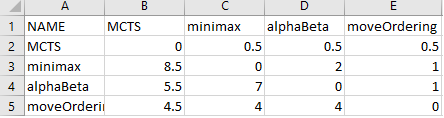
\includegraphics[width=0.7\linewidth]{pics/ExcelSimulation.png}
	\captionof{figure}{ Ergebnisse der Simulation der .csv Datei }
	\label{fig:ExcelSimulation}
\end{minipage}


\subsection{Testing}
Was Simulationen leider nicht schaffen, ist das Finden von gröberen Fehlern, um einen Programmabsturz zu vermeiden.
Um die Stabilität der Software zu verbessern, werden deswegen Tests im Form von Modultests, auch Unit Tests genannt, in die Software integriert.
\\
Dabei beschreibt ein Unit Test das Testen der funktionalen Einzelteile eines Computerprogramms auf ihre korrekte Funktionalität. 
Das bedeutet einzelne Module eines Programmes werden isoliert ohne Interaktion mit anderen getestet. 
Dabei kann es sein, dass externe Komponenten, wie zum Beispiel Datenbanken oder Unterprogramme, simuliert werden müssen. \cite{UnitTestBook}
\\
In der Applikation werden diese Unit Tests in den kritischen Softwarebestandteilen verwendet, welche der Gameserver und der Gameclient sind.
Die Webapp ist weniger fehleranfällig, da es sich lediglich um eine graphische Oberfläche handelt, welche hauptsächlich zur Informationsdarstellung verwendet wird.
Am kritischsten sind dabei die Implementierungen der Spiellogik, der \ac{KI}-Algorithmen-Logik sowie die Netzwerkkommunikation zwischen den Komponenten. 

\subsubsection{Gameserver}
Im Gameserver ist der Zustand des Spieles und die Überprüfung der gespielten Züge enthalten. 
Die Besonderheit beim Testen, befindet sich hier in den Spezialfällen, die in gewissen Damestellungen entstehen können. Beispielsweise muss ein
Spieler in Schlagzwang immer das Schlagen einer Figur ausführen, oder ein Spieler kann nicht noch einmal schlagen, wenn er mit einem Zug bei dem geschlagen worden ist,
eine Dame erhält. Viele dieser Spezialfälle, müssen vor allem in der Implementierung beachtet werden und auch bei Änderung muss beachtet werden, dass 
diese Züge immer noch valide sind. Das führt dazu, dass die Unit Tests immer laufen sollten, nachdem Änderungen an der Spiellogik vorgenommen werden,
um so zu garantieren, dass diese Spezialfälle immer noch funktionieren.
\\
Da es sich beim Gameserver um eine Node.js Anwendung handelt, welche in Typescript implementiert ist, kann eine vorgefertigte Unit Test Library verwendet werden.
Bei dem verwendeten Testing Framework handelt es sich um Mocha, welches zum Testen von Node.js und Javascript Browser Anwendungen benutzt wird. 
Für jeden Testfall einer Funktion wird das tatsächliche Ergebnis mit dem erwarteten verglichen und somit eine Statistik aufgestellt, wie viele Testfälle 
bestanden wurden und wie viele inkorrekt waren. Ein großer Vorteil den Mocha dabei zur Konkurrenz hat, besteht darin, dass die Tests automatisiert ausgeführt werden 
können, sobald der Typescriptcode in Javascript kompiliert wird.
\\ 
Abbildung \ref{fig:UnitTestResult} zeigt das Ergebnis des Mocha Unit Tests, wobei alle 18 Testfälle erfolgreich abgeschlossen wurden.
Bei der letzten Stellung, die auch in der Abbildung dargestellt ist, wird getestet, ob die Software einen Fehler beim zweifachen Schlagen erkennen würde.
Weiß wird durch ``o'' und Schwarz durch ``x'' dargestellt. Das Ausrufezeichen steht für eine Figur, die im Zug davor geschlagen wurde. 
Beim ersten Spielfeld hat Weiß von Reihe 4 Spalte 3 nach Reihe 2 Spalte 5 eine schwarze Figur geschlagen. Da im nächsten Zug die schwarze Figur auf 
Reihe 3 Spalte 6 wegen Schlagzwang geschlagen werden muss, wird auch dieser Zug erwartet. Der Testfall prüft, ob der nächste Zug, der 
vom Test berechnet wird, der richtige weiße Zug ist. Wird stattdessen die bedrohte schwarze Figur gezogen und ein Fehler erkannt, zählt der Testfall als ``passed'', also bestanden.
\\
Die Zeile mit \texttt{nextPlayer} und \texttt{errorMessage} gibt die Nachricht an, welche die Funktion zurückgegeben hat, mit dem Fehler der
mittels \texttt{throw} geschworfen werden würde. \texttt{nextPlayer} steht für die Spieler ID, von welcher der Server den nächsten Zug erwartet.
In diesem Fall steht die ID 0 für Weiß und die ID 1 für Schwarz, wodurch der Server zwei Züge von Weiß, wegen des doppelt Schlagens, erwartet.

\vspace{1em}
\begin{minipage}{\linewidth}
	\centering
	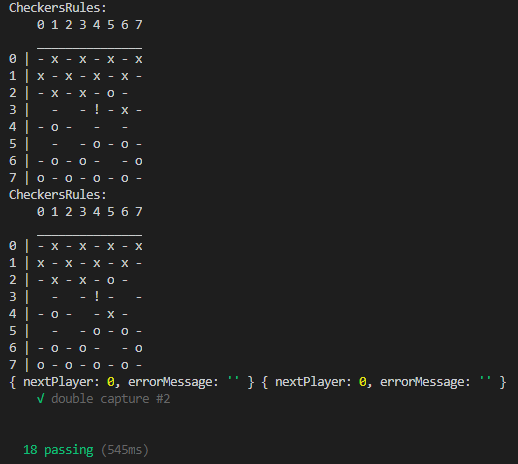
\includegraphics[width=0.6\linewidth]{pics/UnitTestResult.png}
	\captionof{figure}{ Beispiel aus den Unit Tests des Gameservers }
	\label{fig:UnitTestResult}
\end{minipage}

\subsubsection{Gameclient}
Das Testen des Gameclients ist sehr wichtig, da kleinste Fehler zu einer enormen Verschlechterung der Performance des \ac{KI}-Algorithmus führen.
Da die \ac{KI}-Logik als Node.js Add-on implementiert und dadurch in C++ geschrieben ist, kann man nicht einfach ein C++ Testframework benutzen. 
Es sind Funktionen enthalten, die für die Kompatibilität zu Node.js sorgen und nicht mit nativem C++ Compiler zum Laufen gebracht werden können.
Dazu sind die Unit Tests dieser Anwendung als eine Applikation implementiert, welche auf den reinen nativen Teil der Berechnung zugreifen und 
dies modular testen. 
\\
Das Testen der Module läuft ähnlich wie beim Gameserver ab. Es wird entweder allen \ac{KI}-Algorithmen eine komplizierte oder eine sehr einfache Stellung 
übergeben. Diese berechnen anhand ihrer Implementierung den Zug, den sie in dieser Stellung spielen würden und
geben diesen zurück. Er wird daraufhin überprüft und mit dem zuvor definierten Zug verglichen, der erwartet wird, oder welcher in 
komplexen Stellungen definitiv nicht gespielt werden soll. Beispielsweise sind in einer komplexen Stellung sechs Züge möglich. Davon sind drei sehr schwach,
ein Zug ist durchschnittlich gut und die beiden anderen etwas besser. Erwartet wird vom Algorithmus, dass er wenigstens keinen der drei schlechten Züge
auswählt. In sehr einfachen Szenarien muss der Algorithmus den einzigen guten Zug finden, der nicht zum Verlust der Partie führt. 
Außerdem werden in der Testsoftware Parameter der Tiefe und Zeit verändert. Dabei muss jeder Algorithmus auch bei geringem Zeitlimit, die sehr einfachen
Stellungen richtig berechnen. Am Ende wird, wie beim Testframework Mocha, eine Liste mit allen Fällen ausgegeben, die korrekt berechnet wurden.



\pagebreak
% ----------------------------------------------------------------------------------
% Kapitel: Fazit und Ausblick
% ----------------------------------------------------------------------------------
\section{Fazit und Ausblick}
Das Ziel der Arbeit, eine künstliche Intelligenz in die vorhandene Software mit zu integrieren sowie eine Anbindung für mobile Endgeräte zu ermöglichen, wurde erreicht.
Durch die Erweiterungen der graphischen Oberfläche ist es dem Nutzer nun möglich, neben Reversi auch Dame als Spiel zu wählen und dort aus einer 
von vier künstlichen Intelligenzen als Gegner zu wählen, welche über Simulationen in ihrer Spielstärke zueinander validiert sind. 
Zuvor konnte der Benutzer nur über den Touchscreen Eingaben tätigen, um ein Spiel starten zu können,
mit der Erweiterung um eine mobile Anbindung, ist es nun auch möglich mit dem Smartphone ein Spiel zu spielen. 
\\
Ein großes Ziel der Arbeit ist, die Software ebenfalls möglichst erweiterbar zu gestalten, um so eventuell in der Zukunft noch mehr Spiele oder 
mächtigere künstliche Intelligenz Algorithmen, in der Anwendung zu sehen. Durch das Erreichen dieses Zieles können auch zukünftig weitere 
Arbeiten an diese anknüpfen.
Die Benutzeroberfläche hat diesbezüglich ein neues Menü erhalten, aus welchem ein Spiel ausgewählt werden kann. 
So können neue Spiele unabhängig von den bereits vorhandenen zu diesen hinzugefügt werden.
Der Gameserver und der Gameclient haben, in Form eines Interface, ihre klar definierten Schnittstellen für Erweiterungen. 
Da der Gameserver vor allem für Brettspiele konstruiert ist, was aber 
andere Spiele nicht unbedingt exkludiert, ist es nun sehr einfach, ihn um Spiele wie Schach, Mühle oder Go zu erweitern. 
Der Gameclient erlaubt Erweiterungen um weitere künstliche Intelligenz Algorithmen für das Spiel Dame. Es sollte so ohne großen Aufwand möglich sein, 
ihn um Maschine Learning oder andere modernen Algorithmen zu erweitern. Der Netzwerk-Teil des Gameclients kann auch wiederverwertet werden,
um einen Gameclient für ein anderes Spiel zu konstruieren. 
\\
Zusammenfassend kann man sagen, dass die Erweiterungen und Implementierungen der Algorithmen erfolgreich abgeschlossen wurden und hoffentlich 
in der Zukunft von vielen Benutzern bespielt werden.

\pagebreak

% ----------------------------------------------------------------------------------------------------------
% Filter fuer Literatur und Quellen definieren
% ----------------------------------------------------------------------------------------------------------

\defbibheading{Literatur}{\section*{Literaturverzeichnis}} 
\defbibheading{Quellen}{\section*{Quellenverzeichnis}} 
  
\defbibfilter{Literatur}{\not\keyword{online}} 
\defbibfilter{Quellen}{\keyword{online}} 


 ----------------------------------------------------------------------------------------------------------
 Literatur
 ----------------------------------------------------------------------------------------------------------
\lhead{} 
\rhead{Literaturverzeichnis} 

\printbibliography[heading=Literatur,filter=Literatur] 

\pagebreak


% ---------------------------------------------------------------------------------------------------------- 
% Quellen 
% ---------------------------------------------------------------------------------------------------------- 
\lhead{} 
\rhead{Quellenverzeichnis} 

\printbibliography[title = {Quellenverzeichnis}, heading=Quellen,filter=Quellen] 

\pagebreak 

% ----------------------------------------------------------------------------------------------------------
% Anhang
% ----------------------------------------------------------------------------------------------------------
\pagenumbering{Roman}
\setcounter{page}{1}
\lhead{Anhang \thesection}

\begin{appendix}
\section*{Anhang}
\phantomsection
\addcontentsline{toc}{section}{Anhang}
\addtocontents{toc}{\vspace{-0.5em}}

\section{Anforderungsanalyse}
\label{apx:Anforderungsanalyse}
In diesem Kapitel des Anhangs wird zuerst ein beispielhaftes Szenario gezeigt, bei welchem die Software eingesetzt werden soll.
Anschließend werden anhand dieses Szenarios Anforderungen definiert, die von der Software erfüllt werden müssen.
\subsection{Anwendungsszenario}
Will ein Benutzer gegen den \ac{KI} Client spielen, kann er über das Menü auf dem Touch Monitor den \ac{KI}-Algorithmus auswählen und diesen herausfordern.
Dazu kann er, falls er mit seinem Smartphone spielen will, einen QR-Code auf dem Monitor aufrufen, diesen einscannen und dann das Spiel beginnen.
Andernfalls kann der Benutzer auch direkt am Monitor das Spiel starten und auf diesen mittels Touch Züge ausführen.
Die \ac{KI}-Algorithmen, welche auf dem \ac{KI} Client implementiert sind, haben eine Elo Zahl hinterlegt, welche Auskunft über die Spielstärke gibt.
Fühlt sich der Benutzer also über- oder unterfordert, kann er den geeigneten Gegner auswählen. Gibt es mehrere Benutzer, die 
gegeneinander spielen wollen, haben diese die Möglichkeit entweder abwechselnd auf dem Monitor oder beide mithilfe des QR-Code über ihr Smartphone ein Spiel zu starten.
Will ein Benutzer zwei \ac{KI}s beim Spielen beobachten, so kann er diese am Monitor auswählen und gegeneinander antreten lassen.
\subsection{Anforderungen an die Software}
Aus dem oben beschriebenen Anwendungsszenario lassen sich konkrete Anforderungen ableiten, die für die Software von Relevanz sind.
Hierbei wird zwischen funktionalen und nicht funktionalen Anforderungen unterschieden \cite{RequirementEngenieering}.
\subsubsection{Funktionale Anforderungen}
\begin{itemize}
    \item \textbf{/F10/} \textit{Menü zum Auswählen des Spieles:} Die graphische Oberfläche soll dem Benutzer die Möglichkeit bereitstellen, das ein Spiel auszuwählen.
        Dazu soll es ein Menü geben, die möglichen Spiele, wie z.B. Reversi oder Dame, zur Auswahl stellt.
    \item \textbf{/F11/} \textit{Auswählbares Menü für verschiedene \ac{KI} Algorithmen:} Die Applikation muss ein leicht bedienbares graphisches Interface bieten,
        bei welchem verschiedene künstliche Intelligenz Algorithmen ausgewählt und herausgefordert werden können.
    \item \textbf{/F12/} \textit{QR-Code für das Verbinden mit dem Smartphone:} Um einen unkomplizierten Verbindungsaufbau vom Raspberry mit dem Smartphone zu 
        gewährleisten, soll es eine Menü-Option geben, bei der ein QR-Code angezeigt wird. Nach dem Scannen des QR-Codes soll eine Verbindung
        aufgebaut werden, die bis zum Beenden bestehen bleibt.
    \item \textbf{/F13/} \textit{Variable Zeiteinstellung im Menü:} Dem Benutzer soll es möglich sein, über das Menü eine Zeit einstellen zu können, 
        welche jeder Spieler im Spiel für seine Züge zur Verfügung hat. Als Spieler können entweder Benutzer oder \ac{KI} Clients agieren.
    \item \textbf{/F20/} \textit{Benutzer soll Züge ausführen können:} Der Benutzer soll in der Lage sein, Züge gegen die \ac{KI} spielen zu können. Dazu soll er entweder
        direkt über den Touch Monitor oder über das Smartphone eine Eingabemöglichkeit haben. Diese soll den Momentanzustand des Spielbrettes zeigen,
        wodurch der Benutzer eine Entscheidung für seinen nächsten Zug treffen und diese über eine Berührung des Monitors ausführen kann.
    \item \textbf{/F21/} \textit{Benutzer sollen gegen andere Benutzer spielen können:} Für mehrere Benutzer soll es möglich sein, gegeneinander spielen zu können. Dazu sollen sie 
        entweder den Touch Monitor verwenden, indem sie abwechselnd Züge ausführen, oder beide jeweils ein Smartphone.
    \item \textbf{/F22/} \textit{Der Benutzer kann \ac{KI}s gegeneinander spielen lassen:} Der Benutzer soll in der Lage sein zwei \ac{KI}-Algorithmen auszuwählen
        und diese gegeneinander spielen zu lassen. Damit man dieses Spiel sehen kann, sollen alle Züge, die 
        von beiden getätigt werden, auf dem Spielbrett des Touch Monitors angezeigt werden.
    \item \textbf{/F30/} \textit{Eine Elo-Zahl soll die Spielstärke der Algorithmen angeben:} Damit der Benutzer eine für sich angemessene Herausforderung findet,
        sollen schwächere und stärkere \ac{KI}-Algorithmen in der \ac{GUI} gekennzeichnet werden. Um eine genaue Kennzahl für die Stärke zu erhalten, werden die Elo-Zahlen durch
        Simulationen berechnet. Diese Simulationen sind Spiele der Algorithmen untereinander.
   
\end{itemize}
\subsubsection{Nichtfunktionale Anforderungen}
\begin{itemize}
    \item \textbf{/Q10/} \textit{Robustheit der Smartphoneverbindung:} Nach der Verbindung mit dem Smartphone (mittels QR-Code /F12/), muss sichergestellt sein, dass die Verbindung nicht ohne
        Grund abbricht, sondern erst, wenn z. B. die Distanz zwischen Smartphone und Pi zu groß ist. Nach einem Verbindungsabbruch soll 
        das Spiel nicht endgültig abgebrochen werden, sondern eine Möglichkeit zum Wiederverbinden bestehen.
    \item \textbf{/Q20/} \textit{Elo-Zahlen sollen Stärke widerspiegeln:} Die durch die Simulationen errechnete Elo-Zahl von /F30/ soll auch in etwa dem Stärkegrad der Algorithmen entsprechen.
        Hat ein Algorithmus sehr viel mehr Elo, muss er auch dementsprechend stärker sein.
    \item \textbf{/Q30/} \textit{Zeiteinstellung soll von der \ac{KI} berücksichtigt werden:} Die Zeiteinstellung von /F13/ soll vom \ac{KI} Client als Berechnungsdauer genutzt werden.
        Dieser soll dabei seine Rechenzeit so gut wie möglich an die Zeiteinstellung anpassen.
    \item \textbf{/Q40/} \textit{Reaktionszeit des Touch-Interfaces:} Das Berühren des Touch Monitors soll zur sofortigen Ausführung des Befehls der Software führen.
    \item \textbf{/Q50/} \textit{Mobile Responsiveness:} Das Spielfeld soll immer gleich skaliert aussehen, unabhängig davon welches Smartphone verwendet wird. 
        Das Verwenden von Tablets oder das Drehen des Gerätes soll keinen Einfluss auf die Darstellung des Spielbrettes haben.
\end{itemize}
\subsubsection{Zusammenfassung der Anforderungen}
Die identifizierten funktionalen und nichtfunktionalen Anforderungen werden in der Tabelle \ref{tab:Anforderungen} zusammengefasst. 
\vspace{1em}
\begin{table}[!h]
	\centering
	\begin{tabular}{|l|l|l|}
		\hline
		\textbf{ID} & \textbf{Funktionale Anforderung}\\
		\hline
		/F10/ & Menü zum Auswählen des Spieles \\
		\hline
		/F11/ & Auswählbares Menü für verschiedene \ac{KI} Algorithmen \\
		\hline
        /F12/ & QR-Code für das Verbinden mit dem Smartphone \\
		\hline
		/F13/ & Variable Zeiteinstellung im Menü \\
        \hline
		/F20/ & Benutzer soll Züge ausführen können \\
        \hline
		/F21/ & Benutzer sollen gegen andere Benutzer spielen können \\
        \hline
		/F22/ & Benutzer kann \ac{KI}s gegeneinander spielen lassen \\
        \hline
		/F30/ & Eine ELO Zahl soll die Spielstärke der Algorithmen angeben \\
	
		\hline
		\textbf{ID} & \textbf{Nichtfunktionale Anforderung}\\
		\hline
		/Q10/ & Robustheit der Smartphoneverbindung \\
        \hline
		/Q20/ & ELO Zahlen sollen Stärke widerspiegeln \\
        \hline
		/Q30/ & Zeiteinstellung soll von der \ac{KI} berücksichtigt werden \\
        \hline
		/Q40/ & Reaktionszeit des Touch-Interfaces \\
        \hline
		/Q50/ & Mobile Responsiveness \\
		\hline
	\end{tabular}
	\caption{Anforderungstabelle}
	\label{tab:Anforderungen}
\end{table}

\pagebreak

\section{\ac{UML} Klassendiagramm vom gesamten Projekt}
\label{apx:AllClassDiagrams}
\vspace{1em}
\begin{minipage}{\linewidth}
	\centering
	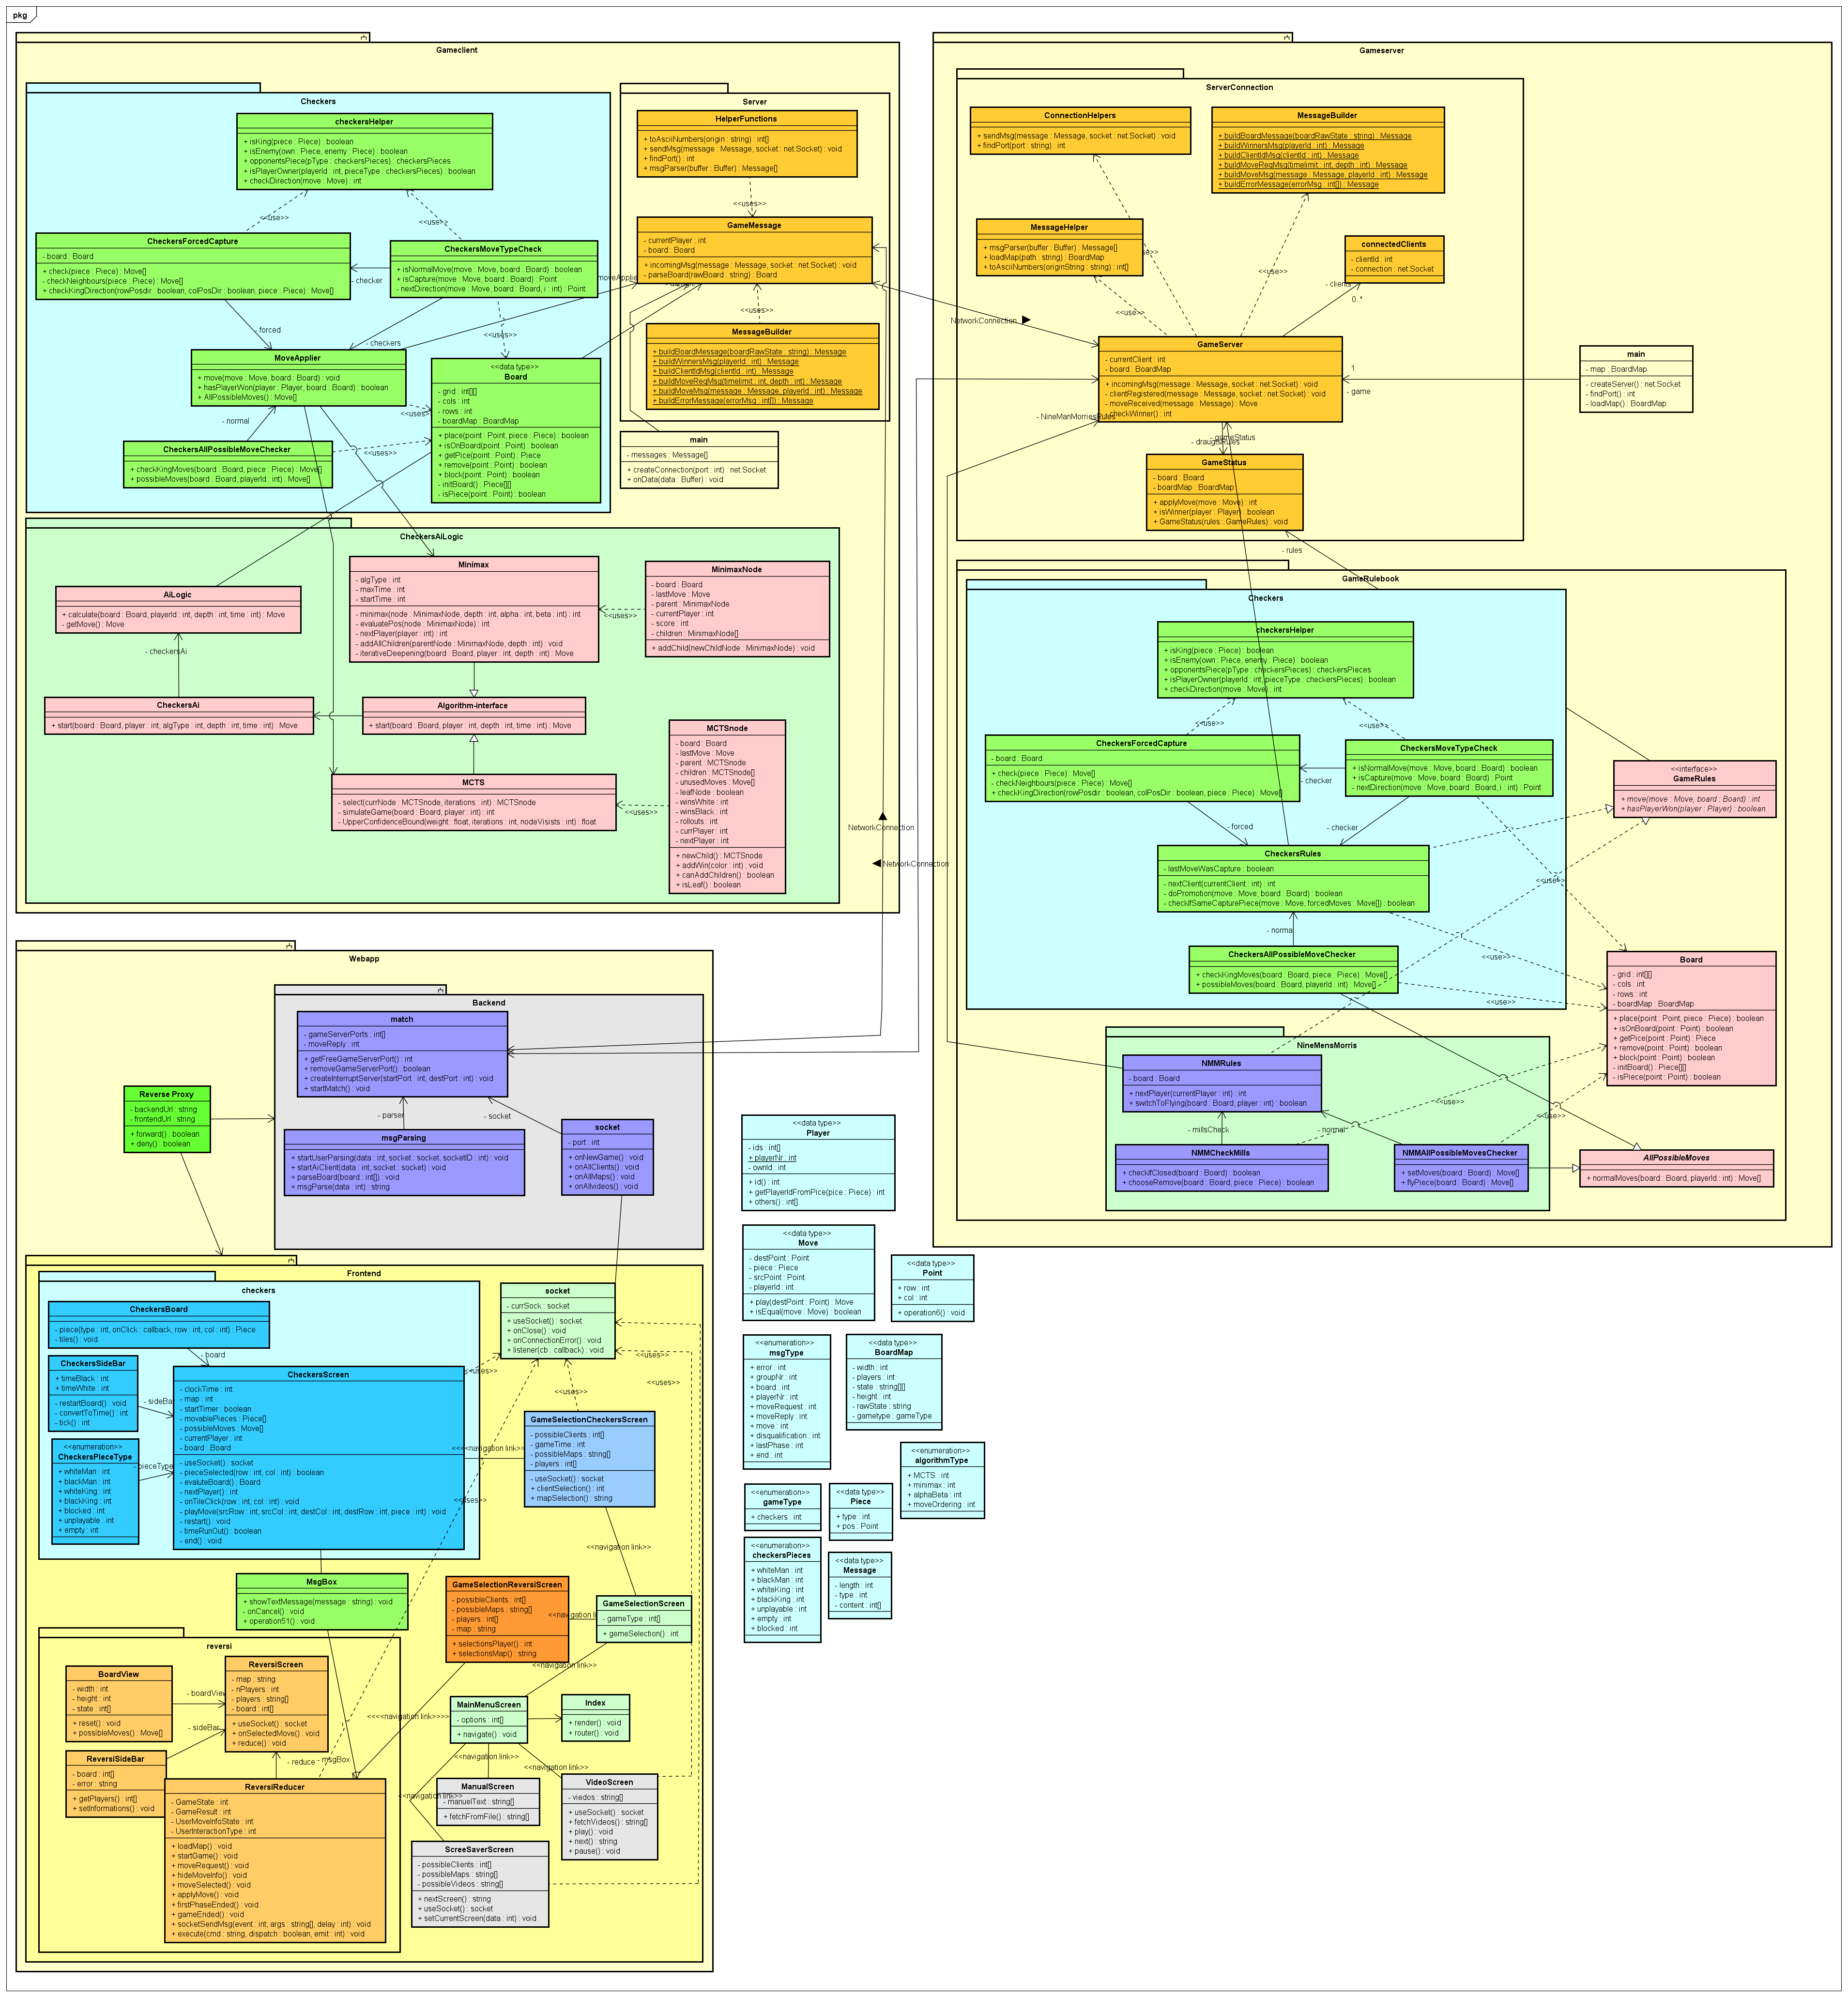
\includegraphics[width=1.0\linewidth]{pics/AllClassDiagrams.png}
	\captionof{figure}{ \ac{UML} Klassendiagramm aller Komponenten des Projektes }
\end{minipage}

Das Diagramm in Abbildung \ref{apx:AllClassDiagrams} zeigt ein \ac{UML} Klassendiagramm, welches alle Komponenten des Projektes zeigt.
Die einzelnen Diagramme, in die es zerlegt werden kann, sind: Der Gameserver in Abbildung \ref{fig:GameServerClassDiagram} auf Seite \pageref{fig:GameServerClassDiagram},
der Gameclient in Abbildung \ref{fig:KIClientClassDiagram} auf Seite \pageref{fig:KIClientClassDiagram} und die Webapp in Abbildung \ref{fig:ReversiXTGUIClassDiagram}
auf Seite \pageref{fig:ReversiXTGUIClassDiagram}. Als Verbindung zwischen den Komponenten ist die Netzwerkkommunikation über Assoziationen gezeigt. 

\pagebreak

\section{Sequenzdiagramme über die Kommunikation der Komponenten}
\label{apx:KommunikationDerKomp}
Die folgenden Abbildungen \ref{fig:UserVsUser} und \ref{fig:AiVsAi} zeigen die beiden anderen Fälle, in 
denen entweder zwei Benutzer oder zwei KIs gegeneinander spielen. Dabei ist Benutzer gegen Benutzer eine einfachere Lösung im Vergleich zu den beiden anderen Varianten, die 
in der Kommunikation möglich sind. Der Gameclient wird nicht benötigt, stattdessen findet die Kommunikation nur zwischen der \ac{GUI} und dem Gameserver statt.

\vspace{1em}
\begin{minipage}{\linewidth}
	\centering
	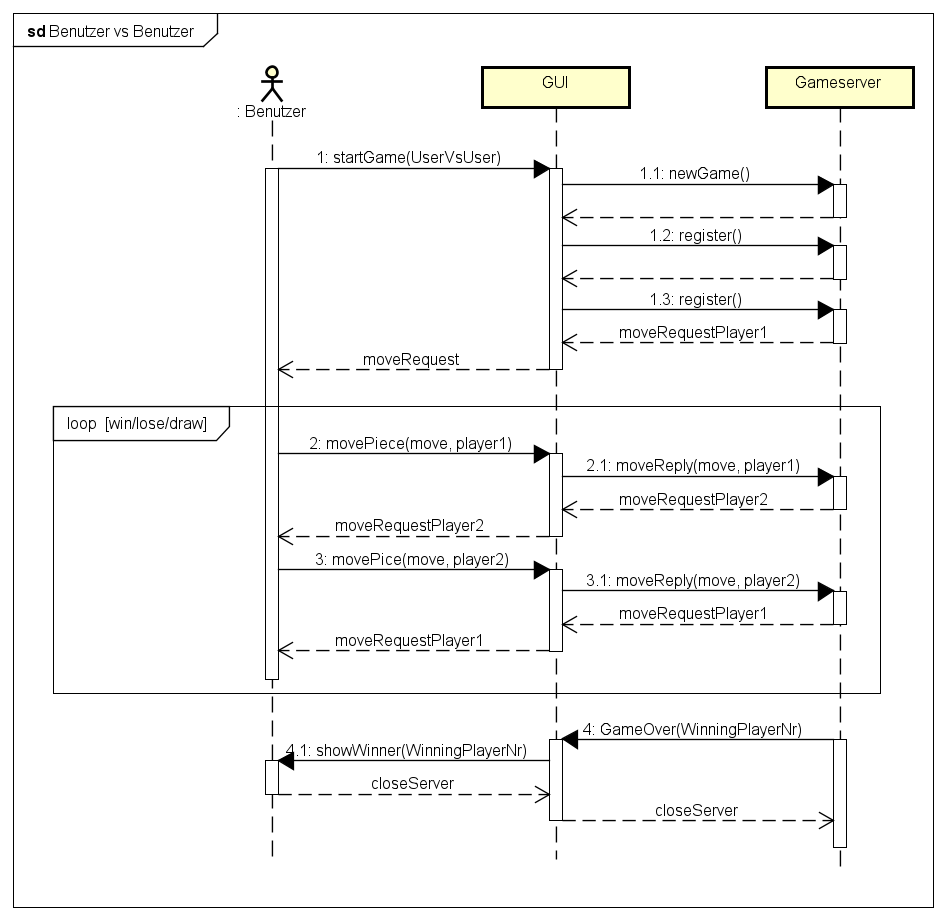
\includegraphics[width=1.0\linewidth]{pics/SequenceDiagramBenutzervsBenutzer.png}
    \captionof{figure}{ \ac{UML} Sequenzdiagramm von Benutzer gegen Benutzer }
    \label{fig:UserVsUser}
\end{minipage}
\\

Die Kommunikation von zwei KIs gegeneinander ist die komplexeste Variante, dazu werden zwei Gameclients gestartet, welche mit dem Gameserver 
kommunizieren. Die \ac{GUI} hört den Gameserver ab, ob Züge gespielt werden, um so ihre Darstellung durch diese zu aktualisieren.

\vspace{1em}
\begin{minipage}{\linewidth}
	\centering
	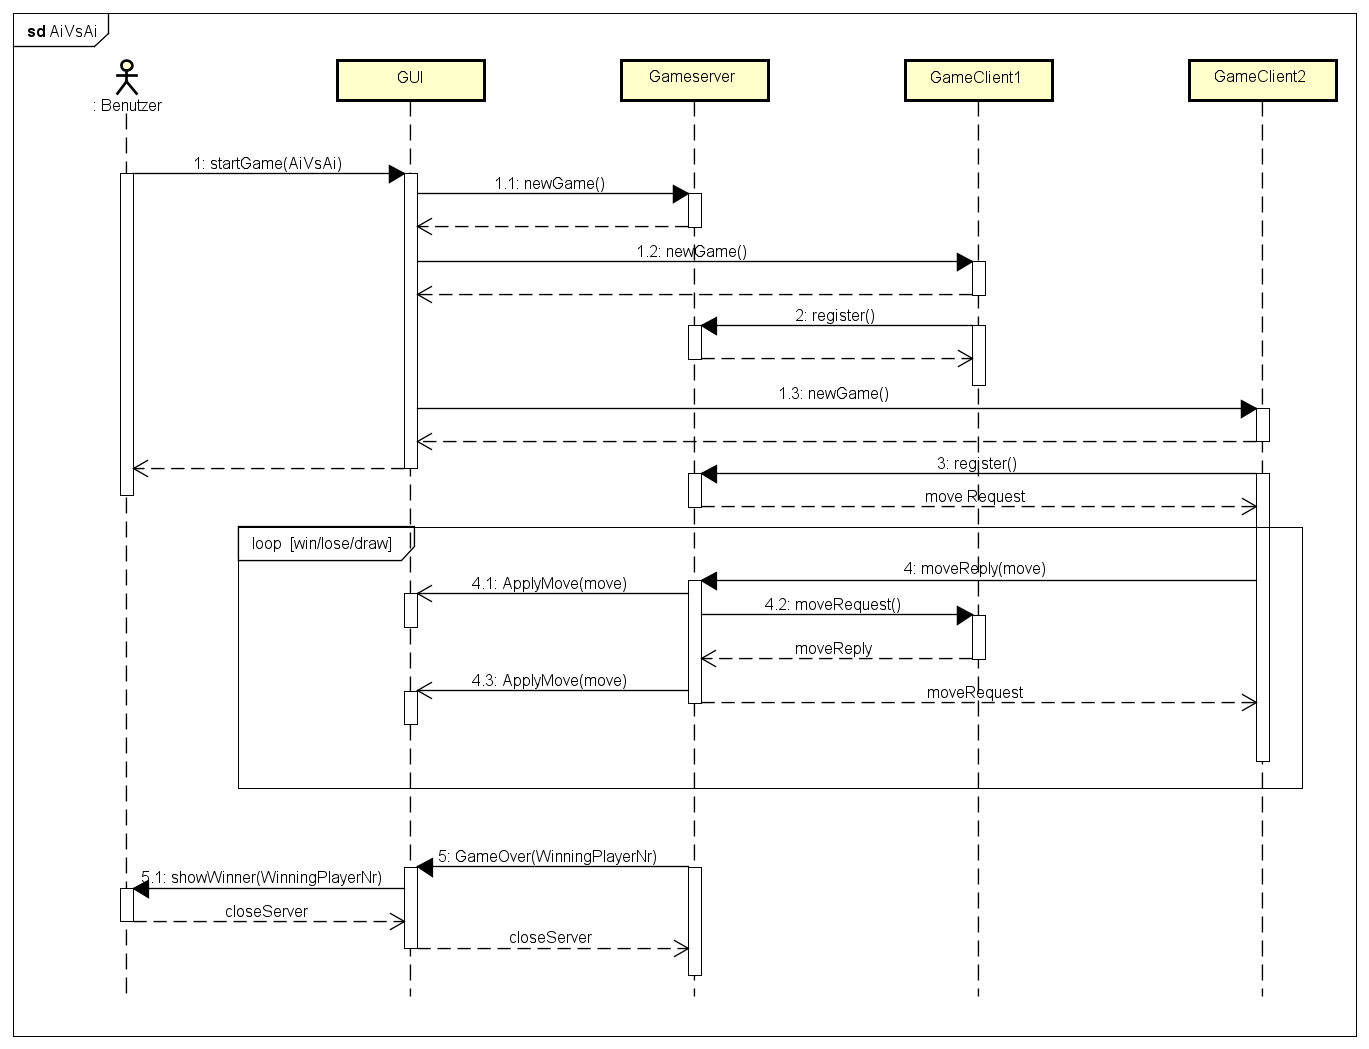
\includegraphics[width=1.0\linewidth]{pics/SequenceDiagramAiVsAi.png}
    \captionof{figure}{ \ac{UML} Sequenzdiagramm von \ac{KI} gegen \ac{KI} }
    \label{fig:AiVsAi}
\end{minipage}

\pagebreak

\section{Nachrichtenprotokoll des Gameservers}
\label{apx:Protokoll}
Das Nachrichten Protokoll des Gameservers besteht aus folgenden Nachrichtentypen:
\begin{itemize}
    \item 0: Fehler. Enthält die Fehlermeldung als String.
    \item 1: Besteht aus der Zeit, die ein Client zur Verfügung hat (32-Bit Integer) und der Gruppennummer des Clients (vorzeichenloser 8-Bit Integer).
    \item 2: Spielfeld. Zuerst die Art des Spieles als vorzeichenloser 8-Bit Integer (z.B 0 für Dame), dann ein vorzeichenloser 8-Bit Integer für die Anzahl der Spieler, die 
    beim Spiel teilnehmen können. Als nächstes zwei vorzeichenlose 8-Bit Integer für die Höhe und Breite des Spielfeldes 
    (Achtung manche Spiele, wie Dame können nur von 2 Spielern gespielt werden!).
    Danach folgen alle Felder des Spielfeldes nach Spezifikation (nicht \textbackslash0 terminiert!).
    \item 3: Spieler-Nummer als vorzeichenloser 8-Bit Integer, die dem Spieler zugewiesen wird.
    \item 4: Zug-Anforderung, bestehend aus einem 32-Bit Integer als Zeitlimit, gefolgt von einem vorzeichenlosen 8-Bit Integer für die maximale Suchtiefe.
    \item 5: Zug-Antwort, besteht aus 4 vorzeichenlosen 16-Bit Integern, welche die Ursprungsspalte und die Ursprungsreihe sowie die Zielspalte und Zielreihe sind.
    Gefolgt von einem vorzeichenlosen 8-Bit Integer für die Angabe der Spielfigurenart (z. B. normale Figur oder Dame).
    \item 6: Normaler Zug, der vom Server validiert worden ist und an alle Teilnehmer geschickt wird. Enthält denselben Inhalt wie die Zugantwort (5), jedoch 
    gefolgt von einem vorzeichenlosen 8-Bit Integer, welcher die Spieler ID beschreibt.
    \item 7: Disqualifikation. Ein vorzeichenloser 8-Bit Integer mit der Spieler ID, welcher disqualifiziert wird.
    \item 8: Letzte Phase, nachdem der Endzustand der ersten Phase erreicht wird (wird in Dame nicht verwendet, aber falls Mühle später relevant wird, z. B. um vom Setzen 
    der Steine zum Springen zu gelangen).
    \item 9: Spielende. Enthält einen vorzeichenlosen 8-Bit Integer mit der Spieler ID des Spielers, der gewonnen hat.
\end{itemize}

\pagebreak

\section{Übergabeparameter von Gameserver und Gameclient}
\label{apx:Parameters}
Da der Gameserver und der Gameclient vom Backend der Webapp gestartet werden, braucht das Backend eine Möglichkeit Parameter zu übergeben, 
um die Auswahl des Spieles oder des Ports zu beeinflussen. Deswegen haben diese Anwendungen Übergabeparameter, die beim Start der
Anwendung angegeben werden können. 
\\\\
Übergabeparameter des Gameservers:
\begin{itemize}
    \item -m: Die Karte mit Pfad zum Ordner.
    \item -p: Der Port, auf dem die Anwendung laufen wird.
\end{itemize}
Beispiel zum starten:\\
\texttt{node dist/src/main.js -m ../checkers\_8x8.map -p 9000}\\
Zu beachten ist, dass nicht die Typescript Datei main.ts benutzt wird, sondern die kompilierte Javascript Datei main.js.
Das Kommando startet einen Gameserver auf Port 9000 mit einem 8x8 Damespielfeld.
\\\\
Übergabeparameter des Gameclients:
\begin{itemize}
    \item -p: Der Port, auf dem der Gameserver läuft, zum Verbinden auf diesen.
    \item -t: Das Zeitlimit pro Zug, falls 0 angegeben wird, wird nur die Tiefe benutzt. Gilt nur, falls der Gameserver
    keine Zeit mit den MoveRequests mitschickt.
    \item -c: Suchtiefe, bis zu welcher Tiefe ein Algorithmus suchen darf, falls jedoch Zeit verwendet werden soll, dann Tiefe gleich null setzen.
    \item -a: \ac{KI}-Algorithmus, welcher ausgewählt wird.
\end{itemize}
Beispiel zum Starten:\\
\texttt{node dist/src/main.js -p 9000 -t 0 -c 5 -a 0} \\
Hier gilt das gleiche wie oben beim Gameserver, bezüglich main.js. 
Dieses Komando startet den Gameclient und verbindet ihn mit dem Gameserver, der auf Port 9000 läuft. Das Zeitlimit ist auf 0, was dazu führt, dass es nicht beachtet wird
und stattdessen die Tiefe 5 benutzt wird. Der angegebene Algorithmus wird mit der Zahl 0 versehen, was \ac{MCTS} entspricht.
Jeder Algorithmus bekommt einen Integerwert zugewiesen, der in der Datei algoriths-consts.js wie folgt gespeichert wird: 
\begin{itemize}
    \item \ac{MCTS} = 0
    \item minimax = 1
    \item alphaBeta = 2
    \item moveOrdering = 3
\end{itemize}

\pagebreak

\section{Ordnerstruktur des Projekts}
Die Ordnerstruktur ist für dieses Projekt etwas speziell, da sie durch die Git Submodule geprägt ist.
Die Abbildung \ref{fig:FolderStructure} zeigt die grobe Ordnerstruktur. Zu beachten ist, dass es sich ein Git Repository handelt und sich
der Gameclient, der Gameserver und die Simulation in dem Ordner BoardGames befinden, welcher wieder ein eigenes Git Repository umfasst. 
Dadurch ist dieses Verzeichnis beim Initialzustand nach dem Klonen des Repositories leer, kann aber über das Initialisieren der Submodules 
mit dem benötigten Inhalt befüllt werden. Der Programmcode befindet sich jeweils im Ordner \texttt{src} und die kompilierten Dateien 
in \texttt{dest}. Das Backend befindet sich im Ordner \texttt{server} und das Frontend in \texttt{webapp}. Die Karten, welche vom Gameserver 
für verschiedene Spiele verwendet werden, befinden sich in \texttt{maps}.

\vspace{1em}
\begin{minipage}{\linewidth}
	\centering
	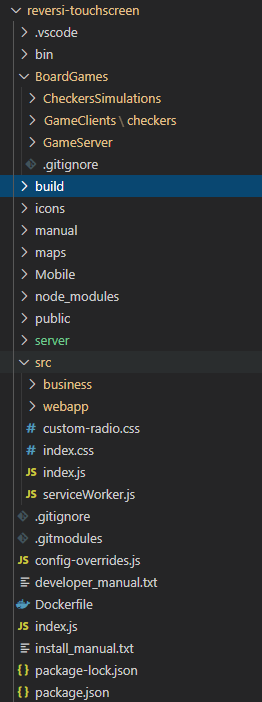
\includegraphics[width=0.3\linewidth]{pics/FolderStructure.png}
    \captionof{figure}{ Ordnerstruktur des Projektes }
    \label{fig:FolderStructure}
\end{minipage}


\pagebreak

\section{Erste Installation}
\label{apx:Installation}
Um die Applikation zu installieren, muss sie erst aus ihrem Git Repository geklont und dann mit ihren Submodulen initialisiert werden.
Erstes Mal Klonen: \\ 
\texttt{git clone https://<User>@bitbucket.org/kernoth/reversi-touchscreen.git} \\
Für \texttt{<User>} muss ein Bitbucket Account angegeben werden, welcher auf das reversi-touchscreen Repository Zugriff hat.
Zum Initialisieren der Submodule (im geklonten Verzeichnis der Anwendung ``/reversi-touchscreen''): \\
\texttt{git submodule update --init --recursive} \\
Dadurch wird der Ordner \texttt{BoardGames} mit den Submodulen initalisiert, auch hier wird wieder Zugang auf das Gitlab Repository
https://gitlab.oth-regensburg.de/kec39902/ba-kibrettspieleundgui-federholzner benötigt. \\
Ist der Ordner BoardGames nach dem Aufruf zum Initialisieren der Submodule immer noch leer, so sind warscheinlich alle Files in Staging gelöscht.
Wenn \texttt{git status} mehrere Files anzeigt ist, das der Fall. Einfach \texttt{git reset .} zum unstagen und \texttt{git checkout -- .} 
eingeben, dann sollte der Ordner mit den fehlenden Dateien befüllt sein. \\ 
Um nun die \texttt{node\_modules} der Javascript Anwendungen zu befüllen: \\
\texttt{npm run postInstall} im Verzeichnis der Applikation (``/reversi-touchscreen'') eingeben um die Installation der node\_modules zu starten. \\
Um Typescript in Javascript und C++ in C zu kompilieren: \\
\texttt{npm run buildAll} \\
Damit auf den Raspberry von außen zugegriffen werden kann, also via mobile Endgeräte, muss der Reverse Proxy Nginx noch installiert werden. \\
Für Windows: Downloaden von https://www.nginx.com/ \\
Für Linux: \texttt{sudo apt-get install nginx} (oder falls andere Distro Anweisungen von https://www.nginx.com/ zur Installation folgen)\\
Danach die \texttt{nginx.conf} Datei, welche sich im Nginx Installations Ordner befindet, durch die \texttt{nginx.conf} Datei aus dem Projekt Ordner
``/reversi-touchscreen'' ersetzen. Dieser Ordner ist bei Linux meist in /etc/nginx, in Windows muss der Ordner bei der Installation angegeben werden.
Es ist zu beachten, dass der Nginx laufen muss, damit er funktioniert.

\pagebreak

\section{Starten der Anwendung}
\label{apx:appStarten}
Das Starten der Anwendung wird von NPM-Scripten übernommen, diese kann man in den \texttt{package.json} Dateien der Software Komponenten finden.
Der Gameserver und der Gameclient haben diese Datei auch, um so alleinstehend gestartet werden zu können. 
In Abbildung \ref{fig:npmScripts} findet man alle Script Kommandos, über welche man die Software bauen bzw. starten kann.
Die wichtigsten Kommandos sind \texttt{runall}, \texttt{buildAll} und \texttt{postInstall}. So wird \texttt{postInstall} zur 
frischen Installation verwendet, um die node\_modules der Komponenten zu installieren. Danach kann erst \texttt{buildAll} aufgerufen werden, 
was für die Kompilierung von React in den Produktions Modus und Typescript in Javascript verantwortlich ist. 
Das Kommando \texttt{runall} startet dann die Anwendung.

\vspace{1em}
\begin{minipage}{\linewidth}
	\centering
	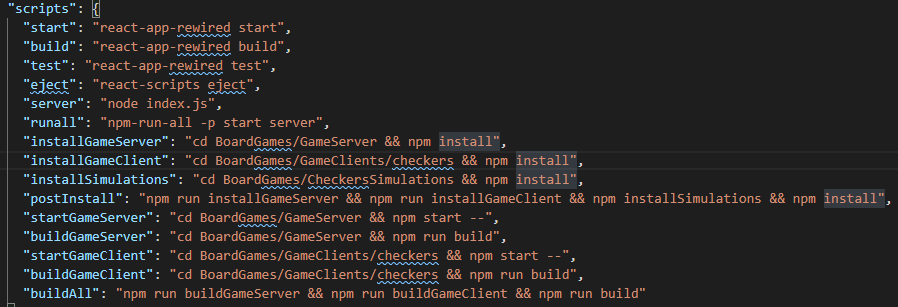
\includegraphics[width=0.7\linewidth]{pics/npmScripts.png}
    \captionof{figure}{ Die NPM Skripte zum Starten der Applikation }
    \label{fig:npmScripts}
\end{minipage}
\\

Ein Beispiel zur Verwendung der Kommandos:
\\
\texttt{npm run runall}
\\
Das Format ist \texttt{npm run <script>}, wobei für \texttt{<script>} eines der in Abbildung \ref{fig:npmScripts} dargestellten Kommandos verwendet werden muss.

\end{appendix}


\pagebreak




\end{document}
